\documentclass[mathematics,article,accept,moreauthors]{Definitions/mdpi}
\usepackage{placeins}
\usepackage{xurl}
\usepackage{tabularx}
\usepackage{algorithm}
\usepackage{algpseudocode}
%\firstpage{1}
%\makeatletter\setcounter{page}{\@firstpage}\makeatother
%\pubvolume{0}\issuenum{0}\articlenumber{0}
%\pubyear{2026}\copyrightyear{2026}
%\datereceived{ }\daterevised{ }\dateaccepted{ }\datepublished{ }
%\doinum{}\hreflink{}




%=================================================================
% MDPI internal commands - do not modify
\firstpage{1} 
\makeatletter 
\setcounter{page}{\@firstpage} 
\makeatother
\pubvolume{1}
\issuenum{1}
\articlenumber{0}
\pubyear{2026}
\copyrightyear{2026}
\externaleditor{Takashi Suzuki and Chuanjun Chen} % More than 1 editor, please add `` and '' before the last editor name
\datereceived{26 September 2026} 
\daterevised{26 October 2026} % Comment out if no revised date
\dateaccepted{30 October 2026} 
\datepublished{ } 
%\datecorrected{} % For corrected papers: "Corrected: XXX" date in the original paper.
%\dateretracted{} % For retracted papers: "Retracted: XXX" date in the original paper.
%\doinum{} % Used for some special journals, like molbank
%\pdfoutput=1 % Uncommented for upload to arXiv.org
%\CorrStatement{yes}  % For updates
%\longauthorlist{yes} % For many authors that exceed the left citation part
%\IsAssociation{yes} % For association journals

%=================================================================


\Title{Positive Joint Laplace Inversion: Spectral Support Selection and Identifiability in Diffusion-Ordered Spectroscopy}
\newcommand{\orcidauthorC}{0000-0001-8355-580X}
\newcommand{\orcidauthorD}{0000-0002-5510-6297}
\Author{Víctor 
 Valdivieso $^{1}$, Marta Gonz\'alez-L\'azaro $^{2}$, Ignacio Fern\'andez $^{2}$\orcidC{} and Francisco Manuel Arrabal-Campos $^{1,2,*}$\orcidD{}}
 
 
 
\AuthorNames{Víctor Valdivieso, Marta González-Lázaro, Ignacio Fernández and Francisco Manuel Arrabal-Campos}



%\AuthorCitation{Valdivieso, V.; Gonz\'alez-L\'azaro, M.; Fern\'andez, I.; Arrabal-Campos, F.M.}
\address{%
$^{1}$ \quad Department of Engineering, Research Centre CIAIMBITAL, Escuela Superior de Ingenier\'ia, University of Almer\'ia, 04120 Almer\'ia, Spain; {mcv598@inlumine.ual.es}\\
$^{2}$ \quad Department of Chemistry and Physics, Research Centre CIAIMBITAL, University of Almer\'ia,\linebreak   04120 Almer\'ia, Spain; {glm332@ual.es} (M.G.-L.); {ifernan@ual.es} (I.F.)}
\corres{Correspondence: {fmarrabal@ual.es}}
\abstract{A small DOSY fitting error does not establish which components are present. We formulate joint positive Laplace inversion for shared diffusion distributions in TRAIn-MF and shared atomic rates in resolution-adaptive inversion (RAI) and diffusion orthogonal moment exchange (DOME). The analysis gives discretization bounds, conditional uniqueness and fixed-rate stability estimates. A common component selector combines residualized kernels, nonnegative variable projection and prediction on reserved acquisitions. Across 36 primary atomic simulations, mean spectral leakage decreases from 5.166\% to 1.728\% for RAI and from 3.857\% to 1.728\% for DOME. A factorial experiment supports contributions from both selection stages without establishing an independent advantage of either proposal mechanism. Additional studies include 300 null matrices, 96 weak-component problems, controlled TRAIn-MF convergence tests, five neural training seeds on 120 new problems, classical references and measured DOSY spectra. Weak components are often missed, some TRAIn-MF fits fail the stationarity check, and the neural accuracy gains remain inconclusive. Classical references predict better on the public multicomponent example. These findings separate the demonstrated reduction in spectral leakage from stronger claims about distributional width, chemical identity or confidence after adaptive selection.}
\keyword{inverse Laplace transform; positive measures; variable projection; nonnegative least squares; model selection; spectral support; identifiability; DOSY}
\MSC{65R32; 65F22; 62F07; 92E10}
\newcommand{\R}{\mathbb{R}}
\newcommand{\one}{\mathbf{1}}
\newcommand{\argmin}{\operatorname*{arg\,min}}
\newcommand{\rank}{\operatorname{rank}}
\newcommand{\diag}{\operatorname{diag}}
\newcommand{\tr}{\operatorname{tr}}
\newcommand{\supp}{\operatorname{supp}}

%\renewcommand{\contentleftcolumn}{\leftcolFont\raggedright
%\textbf{Research manuscript}\\17 October 2026\\[4pt]
%Revised manuscript.}
%\fancypagestyle{plain}{\fancyhf{}\renewcommand{\headrulewidth}{0pt}\renewcommand{\footrulewidth}{0.4pt}
%\fancyfoot[L]{\fontsize{8}{9}\selectfont Research manuscript for Mathematics}
%\fancyfoot[R]{\fontsize{8}{9}\selectfont 17 October 2026}}
%\AtBeginDocument{\fancyhead[L]{\fontsize{8}{9}\selectfont Positive joint Laplace inversion}
%\fancyhead[R]{\fontsize{8}{9}\selectfont\thepage{} of \pageref*{LastPage}}\fancyfoot{}}
\begin{document}
%\input{sections/introduction}


\section{Introduction}
Recovering a positive distribution from a small number of Laplace-transform samples is a prototypical ill-conditioned inverse problem. Diffusion-ordered nuclear magnetic resonance spectroscopy (DOSY) provides a particularly useful setting: the acquisition dimension contains attenuations, while the spectral dimension contains many potentially related signals~\cite{stejskal,morris}. Different chemical shift positions can carry contributions with the same diffusion coefficient, so independent inversion of every spectral channel discards useful structure. Conversely, imposing excessive sharing can spread a fitted component into spectral regions where it is~absent.

Two questions must therefore be separated. The~first is how well a positive measure explains the observations. The~second is which components, if~any, are sufficiently resolved to support an interpretation. A~small residual answers neither the second question nor the question of whether a distribution is atomic or continuous. A~sharply drawn DOSY band can be the consequence of the chosen representation, and~a smooth band can be the consequence of regularization. Neither appearance alone establishes molecular~identity.

Classical approaches address different aspects of Laplace inversion. CONTIN uses constrained regularization~\cite{contin}; TRAIn uses an iterative trust-region construction~\cite{train}; ITAMeD applies iterative thresholding~\cite{itamed}; and PALMA combines entropy and sparsity~\cite{palma}. Regularized Kaczmarz methods provide an algebraic reconstruction perspective~\cite{kaczmarz}. Joint processing is also established: simultaneous inversion with nonnegative low-rank regularization was investigated by Yuan~et~al.\ \cite{silt}, and~high-resolution DOSY reconstruction by Lin~et~al.\ \cite{lin}. These precedents rule out treating joint inversion, positivity, or~a low-rank factorization as novel in~themselves.

Applications to protein and polymer molecular-weight estimation motivate reliable diffusion recovery while requiring a separate, condition-dependent calibration~\cite{arrabal2016,protein,concentration}. Polymerization monitoring, cyclic polymers and chitosan provide related applications~\cite{photo2026,cyclic2021,cyclic2023,chitosan2026}; they do not validate the present reconstruction benchmark. Algorithmic precedents from this research program include the genetic search in diffGA, algebraic reconstruction in dART, and~regularized Kaczmarz inversion~\cite{diffga,dart,kaczmarz}. TRAIn-MF extends the single-channel trust-region method of Xu and Zhang~\cite{train} to shared diffusion profiles~\cite{mfv31}. Section~\ref{sec:mfmath} defines the joint objective.

Finite exponential models introduce a second established lineage. Linear amplitudes can be eliminated from nonlinear least squares by variable projection~\cite{golub}; constrained extensions require attention to active sets and differentiability~\cite{shearer}. Nonnegative least squares (NNLS) supplies the conditional amplitude problem~\cite{lawson}. Continuous sparse-measure methods, including sliding Frank--Wolfe, show that off-grid Laplace support recovery has its own mathematical theory under explicit hypotheses~\cite{denoyelle}. The~method considered here is a finite candidate search with support selection. It is not a new proof of unrestricted super-resolution and does not inherit guarantees from a different~estimator.

Our focus is the interface between representation, optimization, and~selection. We use a positive measure formulation to compare continuous shared profiles with shared atomic rates. We derive the exact local residual derivative on a stable NNLS active set, explain the information in residualized kernels, and~specify a selector that uses spectral coherence without deleting components solely because their heights are small. The~selector is applied to two research implementations from the same development program: resolution-adaptive inversion in its component mode (RAI) and diffusion orthogonal moment exchange (DOME). Their different proposal mechanisms feed a common final estimator, denoted RAI-S and DOME-S. The~suffix identifies spectral-support selection; it does not designate a new acquisition or a distinct physical~model.

The mathematical statements have deliberately limited scope. We prove finite-sampling nonuniqueness for unrestricted positive measures and contrast it with exact uniqueness in a bounded-order noiseless atomic class. We establish a grid-conversion bound, conditional uniqueness of amplitude subproblems, and~conditional Gaussian identities motivating selection. These are transparent consequences and adaptations of established principles, rather than claims of priority. The primary comparison shows a reduction in spectral leakage as well as failures in weak and proportional mixtures. For finite-width profiles, TRAIn-MF uses multifrequency matrix factorization. Its factor count need not equal the number of chemical species.

The organization follows this distinction. Section~\ref{sec:related} positions the work among related inverse problem methods. Section~\ref{sec:theory} gives the measure model and mathematical properties. Section~\ref{sec:methods} formulates each inversion method, including its variables, objective, updates, and~selection target. Section~\ref{sec:algorithm} derives the common support selector and presents its structured pseudocode. Appendix~\ref{app:extensions} gives additional inversion models. Appendix~\ref{app:auditmath} establishes a conditional profile uniqueness criterion and covariance-aware identities without claiming their calibration after adaptive selection. Sections~\ref{sec:experiments} and \ref{sec:results} describe the primary benchmark and extended validation. Appendix~\ref{app:completevalidation} reports the new convergence, factorial, weak-signal, multi-seed learning, classical reference and experimental studies. The~discussion identifies what remains unresolved, including unknown or correlated noise, structural misspecification and independent \mbox{chemical~validation.}



%\input{sections/related}


\section{Related Inverse Problems and Algorithmic~Context}\label{sec:related}

\subsection{Representation, Sharing and~Regularization}
Positive Laplace inversion is a first-kind Fredholm problem in which small singular values limit stable recovery~\cite{discrete,hansen}. The~main methodological distinction is the unknown being estimated. CONTIN and UPEN recover distributions stabilized by smoothing, whereas PALMA combines entropy and sparsity~\cite{contin,upen,palma}. Their penalties express different preferences for admissible solutions; none makes finite observations identify an unrestricted positive distribution. The~nonnegative smoothing framework of Butler, Reeds and Dawson supplies an earlier reference~\cite{brd}.

SCORE uses shared discrete exponential components, while LOCODOSY fits local spectral windows whose orders can differ~\cite{score,locodosy}. These are particularly relevant comparators for the atomic RAI-S and DOME-S models. Global sharing pools evidence across resonances; local fitting limits how much unrelated spectral structure is coupled. Neither choice removes the need to determine which components contribute at each chemical shift position. OUTSCORE provides a further component-resolution approach, and~GNAT makes these distinctions explicit in a common processing environment~\cite{outscore,gnat}. Multivariate curve resolution and nonnegative matrix factorization provide broader precedents for shared-factor models~\cite{mcr,nmf}. In~TRAIn-MF, the attenuation factor is additionally constrained to $KS$ with~a known kernel $K$. Normalizing the profiles removes a scale freedom but not all factorization ambiguity; a profile can remain broad or~multimodal.

Table~\ref{tab:externalmethods} contrasts seven relevant external methods across distributional, component-based and learned representations. It identifies feasible comparisons and their contracts. The~frozen primary benchmark is supplemented by the executed SCORE, LOCODOSY and PALMA-objective comparisons in Appendix~\ref{app:externalcomparison}; the remaining entries are context rather than executed~rankings.
\begin{table}[H]

\caption{Properties and requirements for external comparisons. Availability of source code or trained weights is distinct from validation on a common~dataset.}\label{tab:externalmethods}

\begin{adjustwidth}{-\extralength}{0cm}
%\centering %% If there is a figure in wide page, please release command \centering


\begin{tabularx}{\fulllength}{m{2.7cm}LL}
\toprule
\textbf{Method} & \textbf{Representation and Stabilizing Information} & \textbf{Requirement for a Fair DOSY~Comparison}\\
\midrule
CONTIN~\cite{contin} & Nonnegative distribution; constrained smoothing & Match kernel, grid convention and regularization selection; compare prediction and distributional~error.\\
PALMA~\cite{palma} & Positive distribution; entropy and sparsity & Fix the penalty mixture, noise constraint and stopping rule without test-data~tuning.\\


\bottomrule
\end{tabularx}
\end{adjustwidth}
\end{table}

\begin{table}[H]\ContinuedFloat

\caption{{\em Cont.}}




\begin{adjustwidth}{-\extralength}{0cm}
%\centering %% If there is a figure in wide page, please release command \centering


\begin{tabularx}{\fulllength}{m{2.7cm}LL}
\toprule
\textbf{Method} & \textbf{Representation and Stabilizing Information} & \textbf{Requirement for a Fair DOSY~Comparison}\\
\midrule

UPEN~\cite{upen} & Distribution; locally adapted penalty & Use a verified one-dimensional Laplace implementation, not a second inversion over chemical~shift.\\
SCORE~\cite{score} & Shared discrete components and spectral amplitudes & Declare order selection, initialization, amplitude constraints and computation~budget.\\
LOCODOSY~\cite{locodosy} & Local multivariate fits and local component orders & Derive windows and orders from training data; distinguish local contributions from global~species.\\
DRECT~\cite{drect} & Learned Laplace-NMR reconstruction & Match acquisition sampling, units, normalization and training domain; test distribution~shift.\\
DREAM~\cite{dream} & Learned reconstruction with uncertainty estimates & Match the same input contracts and assess uncertainty calibration on independent~data.\\
\bottomrule
\end{tabularx}
\end{adjustwidth}
\end{table}

The code is available for these methods or related implementations, and~pretrained DOSY checkpoints are available for DRECT and DREAM. This makes direct comparisons feasible but~does not make their interfaces interchangeable. Distributional methods do not natively estimate an atomic order; LOCODOSY's local component count is not a global species count; and a learned model may require sampling or normalization different from the present protocol. Adapters must preserve physical units and the observations used for evaluation. In~particular, two-dimensional relaxation tools~\cite{separable2d,upen2d,mupen} cannot treat the chemical shift axis as a second Laplace dimension. The~primary frozen benchmark does not establish a ranking against these seven external methods. The~additional executed comparisons concern the explicitly attributed implementations, adapters, parameter rules and endpoints in Appendix~\ref{app:externalcomparison}; CONTIN, UPEN, DRECT and DREAM remain unexecuted in that common~protocol.

\subsection{Optimization, Identification and~Learning}
Efficient optimization does not overcome a lack of information. FLINT addresses the computational cost of distribution estimation, and~FISTA supplies convergence results for specified convex objectives~\cite{flint,fista}; those results do not automatically cover a bilinear factorization or adaptive support and order changes. ESPIRA estimates exponential parameters through rational approximation and structured matrices~\cite{espira}. Its sampling assumptions, like the assumptions of any identification theorem, must be checked for the model under consideration~\cite{teicher}. Noiseless uniqueness in a bounded-order atomic class and stable recovery of nearby rates in noise are different~claims.

DRECT and DREAM also obtain information from their training distributions~\cite{drect,dream}. Their evaluation therefore requires independent test cases and checks under distribution shift. RAI-Net has a different role: it changes the order of refinement proposals in an adaptive solver. Neither the term ``learning'' nor use of a physical kernel makes it equivalent to a physics-informed neural network, and~the present selector's conditional Gaussian calculations do not provide DREAM's learned uncertainty model or a calibrated chemical confidence~interval.

The distinction between representation, optimization and evidence extends beyond Laplace NMR. Fractional-diffusion studies compare optimizers for recovering derivative orders and boundary conditions~\cite{fractionalmeta}; hybrid searches have been investigated for reconstruction from incomplete tomographic measurements~\cite{hybridct}. Studies of physics-based neural networks further motivate sensitivity analyses across domain geometry and training hyperparameters~\cite{pinngeometry}. These examples involve different forward operators and unknowns: a fractional partial differential equation, tomographic projection data, and~differential-equation solutions, respectively. They provide methodological context, not direct DOSY performance comparators or validation of~RAI-Net.



%\input{sections/theory}


\section{Positive Measures, Discretization, and~Identifiability}\label{sec:theory}

\subsection{Observation Model and the Meaning of a Diffusion~Distribution}
Let 
 $I_D=[D_{\min},D_{\max}]\subset(0,\infty)$ and let $\mu_\ell$ be a finite nonnegative Borel measure for spectral channel $\ell=1,\ldots,p$. With~acquisition coordinates $b_i\geq0$, $i=1,\ldots,n$, write
\begin{equation}\label{eq:measure}
 Y_{i\ell}=(\mathcal L\mu_\ell)_i+\varepsilon_{i\ell},\qquad
 (\mathcal L\mu)_i=\int_{I_D}e^{-b_iD}\,d\mu(D).
\end{equation}

Here, $b_i$ has units $\mathrm{s\,m^{-2}}$ and $D$ has units $\mathrm{m^2\,s^{-1}}$. For~ideal rectangular gradient pulses, $b=\gamma^2g^2\delta^2(\Delta-\delta/3)$ \cite{stejskal}; other waveforms require their own calibrated encoding factor. Merely writing $b=uv$ does not add independent information when the kernel remains $e^{-Duv}$. We consider pure diffusion, without~exchange, convection, relaxation contrast, or~an estimated baseline. Those effects require a different observation~model.

The benchmark assumes independent $N(0,\sigma^2)$ errors with known $\sigma$. Real signed absorption data are permitted: positivity constrains the reconstructed measure, not every noisy datum. Taking absolute values or clipping negative observations would change this noise model. Spectral channels outside a declared signal mask are unestimated, rather than inferred to contain zero chemical~signal.

Let $D_0>0$ be a reference diffusion coefficient and $x=\log(D/D_0)$, with~$I_x=[a,c]$. The~push-forward measure $\nu$ obeys
\begin{equation}\label{eq:log}
 (\mathcal L\mu)_i=\int_{I_x} k_i(x)\,d\nu(x),\qquad
 k_i(x)=e^{-b_iD_0e^x}.
\end{equation}

If $d\mu=f(D)dD=\rho(x)dx$, then $\rho(x)=D_0e^x f(D_0e^x)$. A~density per unit $D$, a~density per unit $\log D$, and~a bin mass are different quantities. In~particular, the~height of a histogram representing an atom diverges as the bin width tends to zero, while its mass remains~fixed.

\subsection{Mass-Preserving Discretization and a Display Error~Bound}
Let $I_x$ be partitioned into cells $C_h$ of width at most $\delta$. Bin masses are $m_h=\nu(C_h)$; plotting cell densities means displaying $m_h/|C_h|$. If~$Q\nu=\sum_h m_h\delta_{x_h}$, with~$x_h$ the midpoint of $C_h$, then total mass is preserved exactly. This operation does not transform an atom into a physically broadened~component.

\begin{Proposition}[Quantization and forward error]\label{prop:quantization}
For a positive measure $\nu$ of mass $M>0$, midpoint quantization satisfies
\begin{equation}\label{eq:quantization}
 W_1(\nu/M,Q\nu/M)\leq\delta/2,\qquad
 |\mathcal L_i\nu-\mathcal L_iQ\nu|\leq M\delta/(2e).
\end{equation}

\textls[-25]{For two normalized measures $\nu,\eta$, both quantized on such a grid,}
$|W_1(\nu,\eta)-W_1(Q\nu,Q\eta)|\leq\delta$.
\end{Proposition}
\begin{proof}
Transport each point to its cell midpoint. Every displacement is at most $\delta/2$, giving the first bound. Since
$|k_i'(x)|=t e^{-t}\leq e^{-1}$ for $t=b_iD_0e^x\geq0$, integration of the Lipschitz bound gives the second. The~final statement follows twice from the triangle inequality\linebreak   for $W_1$.
\end{proof}

This is an approximation bound, not a resolution theorem. The~atomic solver below evaluates its exponentials at the fitted continuous rates, not at histogram midpoints. Its 256-bin export is used for compatible visualization and a declared binned evaluation. On~$D/D_0\in[0.1,15]$, $\delta=\log(150)/256\simeq0.019573$; native and binned transport comparisons need not agree below this scale. The~one-dimensional formula $W_1(\nu,\eta)=\int|F_\nu-F_\eta|dx$ is classical~\cite{vallender}. Normalized shape is undefined for a zero-mass measure and is treated separately~below.

\subsection{Finite Observations and Restricted Atomic~Uniqueness}
\begin{Proposition}[Ambiguity of unrestricted positive measures]\label{prop:ambiguity}
For any $n$ finite Laplace sampling coordinates and any interval with nonempty interior, there exist two distinct positive measures with the same total mass and identical sampled transforms.
\end{Proposition}
\begin{proof}
Choose $n+2$ distinct points $D_j$ in the interval and form the $(n+1)\times(n+2)$ matrix whose first row is one and whose other rows are $e^{-b_iD_j}$. A~nonzero null vector $v$ exists. Since $\sum_jv_j=0$, it has both positive and negative entries. The~measures $\mu_+=\sum_{v_j>0}v_j\delta_{D_j}$ and $\mu_-=\sum_{v_j<0}(-v_j)\delta_{D_j}$ are positive, nonzero, distinct, and~have equal masses and transforms by construction.
\end{proof}

The proposition is an existence statement about the unrestricted class; it does not say that every positive measure is ambiguous under every finite-dimensional restriction. In~particular, the~following elementary atomic result prevents an overstatement of~impossibility.

\begin{Proposition}[Noiseless uniqueness with a prescribed order bound]\label{prop:atomic}
On a compact positive interval, samples at $b_i=b_0+ih$, $i=0,\ldots,2r-1$, with~$h>0$, distinguish any two measures having at most $r$ atoms.
\end{Proposition}
\begin{proof}
The difference of two such measures has at most $s\leq2r$ distinct support points. Absorb $e^{-b_0D_j}$ into their signed weights and put $z_j=e^{-hD_j}$. Equality of the first $s$ samples gives $\sum_{j=1}^s c_j z_j^i=0$, $i=0,\ldots,s-1$. The~resulting square Vandermonde matrix is nonsingular because the $z_j$ are distinct, so every weight vanishes.
\end{proof}

No stability constant uniform over colliding rates follows from this proof. At~finite noise, nearby exponentials can be almost indistinguishable. If~two components have exactly the same $D$, only their summed spectral amplitudes are observed in Equation~\eqref{eq:measure}; diffusion alone cannot separate them into distinct~species.

For a quantitative statement with \emph{fixed correct rates}, normalize the kernel columns: $B=K\diag(\|k_j\|_2)^{-1}$ and $\beta=\diag(\|k_j\|_2)A$. Let $\mu=\max_{j\ne k}|B_j^\top B_k|$ for $r\geq2$, and~set $\mu=0$ for $r=1$. If~$\gamma=1-(r-1)\mu>0$, Gershgorin's bound gives $\sigma_{\min}(B)\geq\sqrt{\gamma}$. For~$Y=B\beta+E$, $\beta\geq0$, and~its NNLS estimate $\widehat\beta$,
\[
 \|\widehat\beta-\beta\|_F
 \leq\frac{\|E\|_F}{\sigma_{\min}(B)}
 \leq\frac{\|E\|_F}{\sqrt{1-(r-1)\mu}}.
\]

Indeed, the~fitted matrix is the Euclidean projection onto the closed cone generated by $B$; nonexpansiveness gives $\|B(\widehat\beta-\beta)\|_F\leq\|E\|_F$. The~smallest singular value then gives the first inequality. This is an amplitude stability bound for fixed rates, not a rate estimation bound. The~coherence criterion is sufficient and conservative: when $\gamma\leq0$, the~actual $\sigma_{\min}(B)$ may still be~positive.

For two normalized columns, $\sigma_{\min}(B)^2=1-\rho$, where $\rho$ is their correlation. Put $k_i(D)=e^{-b_iD}$, $w_i(D)=k_i(D)^2/\|k(D)\|_2^2$, $\overline b_w=\sum_iw_ib_i$, and~$P_k=kk^\top/\|k\|_2^2$. For~a fixed acquisition design and small physical rate difference $\delta$,
\[
 \begin{aligned}
 1-\rho(D,D+\delta)
 &=\tfrac12\delta^2\operatorname{Var}_{w(D)}(b)+O(\delta^3),\\
 \|(I-P_{k(D)})k(D+\delta)\|_2
 &=\|k(D)\|_2|\delta|\sqrt{\operatorname{Var}_{w(D)}(b)}+O(\delta^2).
 \end{aligned}
\]

These expansions follow by differentiating $k/\|k\|_2$: its $i$th derivative is $(\overline b_w-b_i)k_i/\|k\|_2$. Thus, conditioning depends on the sampled $b$ range as well as rate separation. Under~the fixed-rate, fixed-group assumptions of Proposition~\ref{prop:screen}, equal amplitude $a$ over $m$ independent channels gives detection power
\[
 \Pr(Z_{jG}>z_\alpha)=
 \Phi\!\left(\frac{a\|v_j\|_2\sqrt m}{\sigma}-z_\alpha\right),
 \qquad z_\alpha=\Phi^{-1}(1-\alpha/(rg)).
\]

Consequently, power at least $1-\beta_{\rm miss}$ requires $a\|v_j\|_2\sqrt m/\sigma\geq z_\alpha+\Phi^{-1}(1-\beta_{\rm miss})$. The~two-rate expansion gives a local separation scale proportional to
\[
 \frac{\sigma}{a\|k(D)\|_2\sqrt{m\operatorname{Var}_{w(D)}(b)}}.
\]

This is a design- and SNR-dependent calculation, not a universal minimum gap or a calibrated resolution guarantee for adaptively estimated rates and~groups.

For an atomic model, $Y^0=K(D)A$, where $K_{ij}=e^{-b_iD_j}$ and $A\geq0$. If~$K$ has a full column rank, $\rank(Y^0)=\rank(A)$. When $A=wc^\top$ is proportional across spectral channels, the~clean matrix has rank one even if $w$ has several nonzero entries. The~common decay can still be multiexponential and, under~Proposition~\ref{prop:atomic}'s assumptions, identifiable from noiseless samples. Proportionality removes spectral diversity; it is not by itself a proof of scalar exponential nonidentifiability. Repeated noisy versions can improve precision without increasing matrix~rank.

\begin{Proposition}[What a noise threshold says about rank]\label{prop:rank}
If $Y=Y^0+E$ and $\|E\|_2\leq\tau$, the~number of singular values of $Y$ exceeding $\tau$ is no greater than $\rank(Y^0)$.
\end{Proposition}
\begin{proof}
For $k>\rank(Y^0)$, the~singular-value perturbation inequality gives $s_k(Y)\leq s_k(Y^0)+\|E\|_2\leq\tau$.
\end{proof}

Thus, resolved matrix directions provide a lower count, not an upper bound on hidden rates or chemical species. A~search capped at this count makes an additional predictive modeling choice. This matters for the archived automatic TRAIn-MF procedure, whose cap targets resolved factors. It must not be interpreted as a consistent chemical order~estimator.

\subsection{Distributional Sharing, Normalization, and~Partial~Sharing}\label{sec:sharing}
On a mass grid, a~shared distributional model is $X=SA$, with 
~\begin{equation}\label{eq:mfconstraints}
 S\in\R_+^{q\times r},\quad A\in\R_+^{r\times p},\quad
 \one^\top S=\one^\top.
\end{equation}

The simplex constraint fixes the scaling ambiguity $S_{\cdot j}\mapsto t_jS_{\cdot j}$, $A_{j\cdot}\mapsto A_{j\cdot}/t_j$. It does not fix permutation ambiguity, coincident profiles, or~nonunique factorizations. Each column of $S$ is a distribution and may have several modes; its index is not necessarily a species~label.

A partially shared model is $C=SA+V$, $V\geq0$, on~nonnegative unit-integral basis functions $\phi_h$. Then $\rho_\ell(x)=\sum_h C_{h\ell}\phi_h(x)$ and its total mass is $\sum_j A_{j\ell}+\one^\top V_{\cdot\ell}$. Because~$A=0,V=C$ is feasible for every $C\geq0$, the~private term preserves the full positive basis cone. The~shared rank changes the representation cost rather than the set of attainable total densities. The~decomposition itself is not generally identifiable: for $c_\ell=m_\ell s$, every $A_{1\ell}=tm_\ell,V_{\cdot\ell}=(1-t)m_\ell s$, $0\leq t\leq1$, produces the same~density.

One may regularize this model with
\begin{equation}\label{eq:partial}
 J=\frac{1}{2p}\left[\|\sigma^{-1}(KC-Y)\|_F^2+
 \lambda_s\tr(C^\top QC)+\lambda_p\tr(V^\top GV)\right],
\end{equation}
where $K_{ih}=\int k_i\phi_h$, $G_{hk}=\int\phi_h\phi_k$, and~$Q_{hk}=\int\phi_h'\phi_k'$. The~penalties act on the total-density derivative and the private density, respectively. They are not~interchangeable.

\begin{Proposition}[Conditional uniqueness for one shared profile]\label{prop:partial}
For a fixed unit-mass profile $s$, let $L^\top L=Q$, $F^\top F=G$, and~$T=[K/\sigma;\sqrt{\lambda_s}L]$. If~$G$ is positive definite, $\lambda_p>0$, and~$Ks\ne0$, the~conditional NNLS problem for $(a_\ell,v_\ell)$ has a unique solution.
\end{Proposition}
\begin{proof}
Its design matrix is
\begin{equation}\label{eq:partialdesign}
 B(s)=\begin{bmatrix}Ts&T\\0&\sqrt{\lambda_p}F\end{bmatrix},\qquad
 d_\ell=\begin{bmatrix}y_\ell/\sigma\\0\\0\end{bmatrix}.
\end{equation}

If $B(s)(\alpha,z)^\top=0$, the~lower block gives $Fz=0$, hence $z=0$. Then, $Ts\alpha=0$ implies $\alpha=0$. Full column rank makes the quadratic objective strictly convex, giving a unique constrained minimizer.
\end{proof}

The uniqueness result applies to the conditional subproblem. It does not imply a unique outer profile or molecular decomposition. The partial-sharing model is not included in the primary atomic comparison.

%\input{sections/methods}


\section{Method-Specific Inversion~Problems}\label{sec:methods}

\subsection{Notation, Representation, and~Comparison~Scope}
Let $Y\in\R^{n\times p}$ contain the retained spectral channels, with~acquisition coordinates $b_i$, and~let $\Sigma=(\sigma_{i\ell})$ contain their noise standard deviations. Division by $\Sigma$ below is entrywise; the benchmark uses the common value $\sigma$. We distinguish an atomic kernel $K(d)_{ij}=\exp(-b_i d_j)$ from an integrated basis operator
\begin{equation}\label{eq:integratedbasis}
 B_{ih}=\int_{x_{\min}}^{x_{\max}}e^{-b_iD_0e^x}\varphi_h(x)\,dx,
 \qquad \varphi_h\geq0,\quad \int\varphi_h(x)\,dx=1.
\end{equation}

For the latter, $C_{h\ell}\geq0$ is mass, not density height, and~$BC$ predicts the observations. Integration and discretization are part of the forward model, not a cosmetic change to the DOSY display. In~contrast, exporting continuous atomic rates to 256 display cells does not turn the atomic fit into a 256-parameter~inversion.

Table~\ref{tab:methodcontract} distinguishes the unknowns and selection targets of the methods. In the primary comparison, RAI denotes its finite-component mode. Density RAI, adaptive Haar RAI and RAI-Net solve different estimation problems. Appendix~\ref{app:extensions} describes RAI-FLEX, partial-C, CIRCE and support averaging. Appendix~\ref{app:repro} and Supplementary File S1 give the computational details and study protocols.

\begin{table}[H]

\caption{Mathematical contracts. A~selected representation size is not, in~general, a~chemical species~count.}\label{tab:methodcontract}


%\centering %% If there is a figure in wide page, please release command \centering


\begin{tabularx}{\textwidth}{LLLL}
\toprule
\textbf{Method} & \textbf{Unknowns and Prediction} & \textbf{Coupling or Penalty} & \textbf{Selection~Target}\\
\midrule
TRAIn & $h_\ell\geq0$, $Kh_\ell$ & Independent columns; iterative stopping & Stopping~iterate\\
RAI, atomic & $d,A\geq0$, $K(d)A$ & Shared rates & Native BIC-type~order\\
RAI, density & $C\geq0$, $BC$ & Roughness, ridge, spectral graph & Grid and validation~error\\
Adaptive RAI / RAI-Net & $U\geq0$, $B_{\mathcal T}U$ & Shared Haar details & Tree and penalty; learned action order for~Net\\
DOME & $d,A\geq0$, $K(d)A$ & Shared rates, split/exchange proposals & Native corrected~score\\
RAI-S / DOME-S & $d,A,H$, $K(d)A$ & Allowed spectral support $H$ & Predictive order and~support\\
TRAIn-MF & $S,A\geq0$, $KSA$ & Simplex profiles, curvature and ridge & Resolved predictive~factors\\
\bottomrule
\end{tabularx}

\end{table}


\subsection{TRAIn: Squared Positivity and a Trust-Region~Iteration}\label{sec:trainmath}
The supplied single-channel implementation uses a TRAIn-derived trust-region Gauss--Newton iteration~\cite{train}. Its numerical core minimizes the unpenalized residual through the squared parametrization
\begin{equation}\label{eq:trainobjective}
 h=\eta\odot\eta,\qquad f(\eta)=\|Kh-y\|_2^2,
 \quad g=4\diag(\eta)K^\top(Kh-y).
\end{equation}

The Gauss--Newton matrix and trust-region subproblem are
\begin{equation}\label{eq:trainstep}
 B_{\rm GN}=8\diag(\eta)K^\top K\diag(\eta),\qquad
 \min_{\|s\|_2\leq\Delta}\ g^\top s+\tfrac12s^\top B_{\rm GN}s.
\end{equation}

The exact Hessian additionally contains $4\diag(K^\top(Kh-y))$; the code deliberately uses the Gauss--Newton approximation. Truncated conjugate gradients approximate \mbox{Equation~\eqref{eq:trainstep},} stopping at the radius boundary or on nonpositive curvature, with~at most 100 inner iterations. The~trial point is $\eta^+=|\eta+s|$, which leaves its squared physical prediction unchanged. With~a positive predicted reduction, the~acceptance ratio is
\begin{equation}\label{eq:trainratio}
 \rho=\frac{f(\eta)-f(\eta^+)}{-g^\top s-s^\top B_{\rm GN}s/2}.
\end{equation}

The supplied implementation accepts when $\rho>0.01$, halves the radius when $\rho\leq0.25$, and~doubles it when $\rho\geq0.75$, subject to its initial radius cap. These are the settings of the inspected file, not a claim that every published TRAIn implementation has\mbox{ identical~defaults.}

First, it computes $h_{\rm NNLS}=\argmin_{h\geq0}\|Kh-y\|_2$ and $\nu=\|Kh_{\rm NNLS}-y\|_2$. Iteration stops when $\sqrt{f}\leq\mathtt{termFac}\,\nu$ or the iteration budget is exhausted. Thus, $\nu$ is a residual floor from the same data, not an independently measured noise level. Despite a Tikhonov description in the interface, this core contains no explicit term $\lambda\|Lh\|^2$: its regularizing effects come from the parametrization, initialization, and~stopping. Its final threshold $h_j<10^{-6}\max_kh_k$ is a further output~modification.

Squared positivity also changes stationarity: $\eta=0$ gives $g=0$ even when $K^\top(Kh-y)$ has negative entries and the NNLS KKT conditions fail. Indeed, the~supplied initialization is proportional to $\min_i|y_i|$ and becomes zero if that minimum is zero. Consequently, small $g$ is not by itself a certificate of NNLS optimality. Independent calls at each spectral channel minimize a separable sum of these residuals; they impose no shared components across spectral~channels.

\subsection{RAI in Finite-Component~Mode}\label{sec:raiatomic}
For each candidate order $r$, RAI profiles out the amplitudes:
\begin{equation}\label{eq:raiobjective}
 \psi_r(z)=\min_{A\geq0}\frac12\|(K(D_0e^z)A-Y)/\Sigma\|_F^2,
 \quad z\in[\log(D_{\min}/D_0),\log(D_{\max}/D_0)]^r.
\end{equation}

Here, $D_0=\sqrt{D_{\min}D_{\max}}$ in the component implementation. At~each evaluation, SciPy NNLS solves the weighted amplitude problem separately for each spectral channel. Dividing a data column and its noise by the same positive scale, and~rescaling its amplitude variable accordingly, leaves Equation~\eqref{eq:raiobjective} unchanged. The~native code uses $s_\ell=\max(\max_i|Y_{i\ell}|,\operatorname{median}_i\sigma_{i\ell})$ for this conditioning~step.

On a stable NNLS active set, the~envelope gradient is
\begin{equation}\label{eq:raigradient}
 \frac{\partial\psi_r}{\partial z_j}
 =\sum_\ell A_{j\ell}(\partial_{z_j}k_j)^\top
       \bigl((K A-Y)_\ell/\Sigma_\ell^2\bigr),
 \qquad (\partial_{z_j}k_j)_i=-b_i d_j e^{-b_id_j}.
\end{equation}

Bounded L-BFGS-B updates the log rates. This native RAI step is not the squared-amplitude TRAIn trust-region iteration. Ten starts combine an interior equispaced grid, up~to three births chosen by residual improvement on a 49-point log-rate grid extending the preceding order and~seeded random starts. The~lowest attained objective determines the candidate, with~a nearly tied converged start preferred within the implementation's objective tolerance. This is a finite multistart search, not a global minimization~theorem.

The native selector includes $r=0$ and minimizes
\begin{equation}\label{eq:raibic}
 \mathrm{BIC}_{\rm RAI}(r)=2\psi_r+r(p+1)\log(np).
\end{equation}

It counts every amplitude, including zeros. The~primary comparison caps $r$ at four. This score is a heuristic adaptation of BIC~\cite{schwarz}: inactive amplitudes and coincident rates make the mixture singular, invalidating a direct appeal to regular-model dimension counting~\cite{watanabe}. Native optimization statuses are saved; the native selection itself does not enforce the stronger eligibility checks subsequently imposed by RAI-S. There is no spectral graph or density smoothing penalty in this atomic RAI~objective.

\subsection{RAI with a Positive Density and a Spectral~Graph}\label{sec:raidensity}
Let log bins have widths $w_h$ and centers $c_h$, and~use the unit-integral indicator bases in Equation~\eqref{eq:integratedbasis}. The~operator is evaluated by 12-point Gauss--Legendre quadrature per cell. Let $H_w=\diag(1/w_h)$ and define the density-difference operator by
\begin{equation}\label{eq:rairough}
 (RC)_{h\ell}=\frac{C_{h+1,\ell}/w_{h+1}-C_{h\ell}/w_h}
 {\sqrt{c_{h+1}-c_h}}.
\end{equation}

In the solver's column-normalized units, the~fixed-grid, fixed-graph problem is

\begin{equation}\label{eq:raidensity}
 \min_{C\geq0}\ \frac{\|(BC-Y)/\Sigma\|_F^2}{2n}
 +\frac{\lambda_s}{2}\|RC\|_F^2
 +\frac{\eta}{2}\tr(C^\top H_wC)
 +\frac{\gamma}{2}\tr(H_w C L_g C^\top).
\end{equation}

Here $L_g=\diag(W\one)-W$ is a symmetric positive semidefinite graph Laplacian on spectral channels. The~identity $\tr(H_w C L_g C^\top)=\sum_{\ell<m}W_{\ell m}\|H_w^{1/2}(C_\ell-C_m)\|_2^2$ shows that this penalty rewards similar density shapes at connected spectral channels. It is not a chemical assignment constraint. Unlike the unregularized atomic objective, column normalization here also defines the relative scale of the density prior; physical masses are restored after~fitting.

The graph is constructed from normalized training decays, retaining sufficiently informative signals, mutual nearest neighbors, and~a noise-scaled shape-distance threshold. Defaults are SNR at least eight, at~most three mutual neighbors, distance at most 1.5, and~weight $e^{-\mathrm{distance}}$; the precise distance is given in Appendix~\ref{app:graphdetails}. With~the graph held fixed, the~gradient is
\begin{equation}\label{eq:raidensitygrad}
 \nabla F=B^\top((BC-Y)/\Sigma^2)/n
       +\lambda_sR^\top RC+\eta H_wC+\gamma H_w C L_g.
\end{equation}

The defaults $(\lambda_s,\eta,\gamma)=(0.02,10^{-5},0.05)$ give a strictly convex quadratic because $\eta H_w\succ0$. Nonnegative L-BFGS-B uses a diagonal Hessian scaling. The~exact fixed-grid minimizer is therefore unique. The~implementation records a library termination flag and an unscaled projected-gradient residual; it does not compute a certified distance to that minimizer. Termination by a small objective change alone is insufficient to assert accurate first-order stationarity in an ill-conditioned quadratic. Fixed-grid uniqueness also does not establish identifiability of a continuous measure or optimality of the grid~search.

Resolution adaptation starts from 128 bins, proposes midpoint splits while conserving parent mass, and~allows at most 256 bins. For~a candidate split, let $t_h=(k_{h,L}-k_{h,R})/2$. Its score is the sum across spectral channels of squared residual correlations divided by $\|t_h/\Sigma_\ell\|^2$. Splits require sufficient signal information, $\max_\ell\|t_h C_{h\ell}/\Sigma_\ell\|_2/\sqrt n\geq0.25$. Up~to a third of current cells are proposed. A~refined grid is accepted only with successful inner optimization and a validation MSE below $0.99$ of its predecessor; otherwise refinement stops. The~column scale is estimated from fitting rows and retained, while the spectral graph is rebuilt using all supplied reconstruction rows for the final fit on the selected grid. This chooses resolution, not the number of molecular~species.

\subsection{Adaptive Haar RAI: A Convex Problem on Each~Tree}\label{sec:raiadaptive}
The adaptive solver used by RAI-Net is a separate construction. It uses fitting-row scales $s_\ell=\max(\max_{i\in T}|Y_{i\ell}|,8\operatorname{median}_{i\in T}\sigma_{i\ell})$, retained for the final refit. Both the data and noise are divided by these scales, and~physical masses are restored afterwards. A~dyadic tree $\mathcal T$ partitions a 256-cell fine log grid into $m$ active leaves, initially eight and at most 64. If~leaf $j$ has width $w_j$, let $U_{j\ell}$ denote its mass divided by $\sqrt{w_j}$. The~mass-preserving prolongation and observation matrix are
\begin{equation}\label{eq:raiprojection}
 (P_{\mathcal T})_{hj}=\frac{\Delta x_h}{\sqrt{w_j}}\one_{\{h\subset j\}},
 \qquad C=P_{\mathcal T}U,\qquad B_{\mathcal T}=B_{\rm fine}P_{\mathcal T}.
\end{equation}

Let $Q_{\mathcal T}$ be the orthogonal Haar transform of these normalized leaf coefficients; its first row represents total mass. In~normalized data units, joint adaptive RAI solves
\begin{equation}\label{eq:raihaar}
 \min_{U\geq0} F_{\mathcal T,\lambda}(U)
 =\frac{\|(B_{\mathcal T}U-Y)/\Sigma\|_F^2}{2n}
 +\frac{\eta}{2}\|U\|_F^2
 +\lambda\sqrt p\sum_{h=2}^{m}\|(Q_{\mathcal T}U)_{h,:}\|_2,
 \quad \eta=10^{-4}.
\end{equation}

The group penalty promotes shared locations of density changes across spectral channels while leaving their amplitudes distinct. The~separate-spectral channel variant replaces it by $\lambda\sum_{h\geq2,\ell}|(Q_{\mathcal T}U)_{h\ell}|$. Neither penalizes the root coefficient. The~joint penalty is convex; the ridge makes each fixed-tree problem strictly~convex.

For $\lambda>0$, introduce $V=U\geq0$ and $Z=QU$. Write $A_\ell=\diag(\Sigma_\ell^{-1})B_{\mathcal T}/\sqrt n$, $y'_\ell=Y_\ell/(\sqrt n\Sigma_\ell)$, $H_\ell=A_\ell^\top A_\ell+\eta I$, and~$c_\ell=A_\ell^\top y'_\ell$. With~scaled duals $d_V,d_Z$ and $\rho=0.5$, the~implemented ADMM steps are
\begin{align}
 (H_\ell+2\rho I)U_\ell^+&=c_\ell+\rho\{V_\ell-d_{V,\ell}+Q^\top(Z_\ell-d_{Z,\ell})\},\label{eq:raiadmm}\\
 V^+&=[U^++d_V]_+,\qquad Z^+=\operatorname{prox}_{\lambda\sqrt p\,\|\cdot\|_{2,1}^{\rm detail}/\rho}(QU^++d_Z),\nonumber\\
 d_V^+&=d_V+U^+-V^+,\qquad d_Z^+=d_Z+QU^+-Z^+.\nonumber
\end{align}

The proximal map leaves the first row unchanged and sends a detail row $z$ to $(1-\lambda\sqrt p/(\rho\|z\|_2))_+z$. For~$\lambda=0$, an~augmented ridge NNLS problem is used instead. A~feasible primal value and a feasible dual bound give a computable gap; the archived stopping rule is gap $\leq10^{-5}(1+F)$, with~at most 3000 iterations. Appendix~\ref{app:haargap} gives the actual dual construction, so numerical convergence does not depend only on a library success~flag.

Tree actions include joint and private residual-detail splits, position-sensitive and occupied-region splits, and~sibling merges. Split scores remove numerically visible nuisance tangent directions before correlating residuals with a mass-redistribution contrast. At~fixed $\lambda$, a~split is accepted only if both inner solves meet their gap criterion and
\begin{equation}\label{eq:raiaction}
 F_{\rm old}-F_{\rm new}>\max\{10^{-9}(1+F_{\rm old}),\mathrm{gap}_{\rm old}+\mathrm{gap}_{\rm new}\}.
\end{equation}

Merges allow a loss within $10^{-10}(1+F_{\rm old})$. Visited trees are excluded. The~deterministic solver evaluates the available proposals and favors the lowest objective, then fewer leaves. These checks compare attained objectives across representations; they are not a convexity theorem for the whole adaptive search. Completed paths for $\lambda\in\{0,0.01,0.1\}$ are compared by noise-standardized internal validation MSE. Among~paths within 0.005 of the minimum, the~largest $\lambda$ is chosen, then the selected tree is refitted on all reconstruction rows. Validation selects completed paths; it does not replace Equation~\eqref{eq:raiaction} for intermediate~actions.

\subsection{RAI-Net: Learning the Order of Admissible~Actions}\label{sec:rainetmath}
RAI-Net retains Equations~\eqref{eq:raihaar}--\eqref{eq:raiaction}. For~a tree state and a proposed action $a$, it predicts a scalar priority
\begin{equation}\label{eq:rainet}
 q_\theta(\phi_a)=w_3^\top\tanh\!\left(W_2\tanh(W_1\widetilde\phi_a+b_1)+b_2\right)+b_3,
 \qquad \widetilde\phi_a=(\phi_a-\mu)/s.
\end{equation}

The 14 features encode current and proposed tree sizes, action type, conditional and raw residual scores, information, occupied mass, affected width, penalty, data dimensions, and~the current objective; Appendix~\ref{app:netfeatures} specifies them. Feature standardization is fitted on training records only, with~each scale at least 0.1. No true diffusion rates or species count are inference~inputs.

For recorded action gain $g_a$, let $t_a=\operatorname{sign}(g_a)\log(1+|g_a|)$. Training minimizes
\begin{equation}\label{eq:netloss}
 \frac1N\sum_{a=1}^N\ell(q_\theta(\phi_a)-t_a),\qquad
 \ell(e)=\begin{cases}e^2/2,&|e|<1,\\|e|-1/2,&|e|\geq1.\end{cases}
\end{equation}

The original policy's target is training-objective decrease. In~the retrained policy, it is noise-standardized internal validation prediction-MSE decrease; failed actions receive \mbox{$g_a=-1$.} The~latter uses two 48-unit hidden layers, full-batch Adam with learning rate 0.003, 400 epochs, and~seed {9,252,026}. Whole-problem training and validation partitions, rather than random action-row splits, avoid sharing a problem across these partitions. The~bank and checkpoint selection are documented in Section~\ref{sec:experiments}. Changing the target and the training bank together means this is a policy comparison, not an isolated architecture~ablation.

At inference, actions are sorted by decreasing $q_\theta$. With~the archived shortlist of one, evaluation continues until a numerically admissible action is available; failed proposals lead to further candidates. Invalid policy output falls back to the deterministic order. The~accepted action must still satisfy the classical gap and descent checks. The~network therefore neither returns a density directly nor classifies the number of components. Its ordering can change the finite search path because not every action is evaluated: numerical safeguards are retained, but~equality with deterministic RAI's final answer is not~guaranteed.

\subsection{DOME: Atomic Inversion with Moment-Based~Proposals}\label{sec:domemath}
DOME uses a common known $\sigma$ and solves the corresponding fixed-order atomic residual problem in Equation~\eqref{eq:raiobjective}; its difference lies in proposal generation, nonlinear refinement, and~native model selection. It normalizes the whole matrix and noise by $\max(\max|Y|,\sigma)$. Internally it uses $D_{\rm ref}=10^{-9}\,\mathrm{m^2\,s^{-1}}$, $t_i=b_iD_{\rm ref}$, $\delta_j=d_j/D_{\rm ref}$, and\linebreak  $u_j=\log(\delta_j/\delta_{\min})/\log(\delta_{\max}/\delta_{\min})\in[0,1]$. Thus
\begin{equation}\label{eq:domegradient}
 \partial_{u_j}k_j=-t\,\delta_j\log(\delta_{\max}/\delta_{\min})\odot k_j.
\end{equation}

At fixed rates, the~small NNLS problem is solved by enumerating all active subsets, including the empty subset, using SVD least squares. A~bounded trust-region reflective solve then uses the full active-set residual Jacobian of Proposition~\ref{prop:derivative}. This is distinct from native atomic RAI's L-BFGS-B envelope-gradient search and from original TRAIn's squared-amplitude~iteration.

The following proposal equations use these dimensionless rates and acquisition coordinates. A~split of mass $a$ at rate $m$ into $\pi a$ at $m-(1-\pi)\Delta$ and $(1-\pi)a$ at $m+\pi\Delta$ preserves mass and first moment. At~fixed $t$,
\begin{equation}\label{eq:split}
 Y_{\rm split}(t)-ae^{-tm}
 =\tfrac12 ae^{-tm}t^2\pi(1-\pi)\Delta^2+O(\Delta^3).
\end{equation}

Let $E=KA-Y$, $P_K=KK^+$, and~$J$ denote the profiled residual Jacobian in the internal normalized units. With~consistent rate units, a~curvature proposal for component $j$ uses
\begin{equation}\label{eq:domecurvature}
 h_j=(I-P_K)(t^2\odot k_j/2),\quad
 q_j=(I-JJ^+)\operatorname{vec}(h_j A_{j,:}),\quad
 \widehat v_j=\left[-\frac{\langle\operatorname{vec}E,q_j\rangle}{\|q_j\|_2^2}\right]_+.
\end{equation}

Zero or numerically negligible denominators provide no informative direction. A~complementary spectral contrast uses
\begin{adjustwidth}{-\extralength}{0cm}
%\centering %% If there is a figure in wide page, please release command \centering
\begin{equation}\label{eq:domespectral}
 v_j=(I-P_K)(-t\odot k_j),\qquad
 \zeta_\ell=-\tanh\!\left(\frac{v_j^\top E_\ell}{\max(\sigma\|v_j\|_2,10^{-15})}\right),\qquad
 T_{i\ell}=v_{j,i}A_{j\ell}\zeta_\ell.
\end{equation}
\end{adjustwidth}

Its candidate half-separation is $\widehat s_j=[-\langle E,T\rangle/\|T\|_F^2]_+$. The~implementation proposes standard deviation scales $s\in\{\sqrt{\widehat v_j},\widehat s_j,0.12\delta_j,0.4\delta_j,0.85\delta_j\}$ and fractions\linebreak   $\pi\in\{0.15,0.5,0.85\}$, setting $\Delta=s/\sqrt{\pi(1-\pi)}$ before restricting the pair to the physical bounds. Every proposal is evaluated with exact exponentials, not with the \mbox{truncated~expansion.}

Pairwise exchanges use aggregate masses $M_j=\sum_\ell A_{j\ell}$. Given a pair's mass-normalized mean $m$ and variance $v$, alternative fractions \mbox{$\pi\in\{0.08,0.2,0.5,0.8,0.92\}$ yield}
\begin{equation}\label{eq:domeexchange}
 \delta_L=m-\sqrt{v(1-\pi)/\pi},\qquad \delta_R=m+\sqrt{v\pi/(1-\pi)}.
\end{equation}

This preserves the pair's aggregate first two moments at proposal construction. It does not preserve each spectral channel's moments, and~subsequent NNLS refinement is not constrained to preserve them. A~finite beam, distinct-seed filtering, and~local refinement limit the search. Physical rates are returned as $d_j=D_{\rm ref}\delta_j$; the internal numerical floors apply before this conversion. The~native selector includes the zero model and minimizes
\begin{equation}\label{eq:domescore}
 \mathrm{score}_{\rm DOME}=\mathrm{RSS}/\sigma^2+2d_f+
 \frac{2d_f(d_f+1)}{\max(np-d_f-1,1)},
 \quad d_f=r+\#\{A_{j\ell}>10^{-10}\},
\end{equation}
where the amplitude cutoff is in DOME's normalized units. This is a heuristic effective-parameter count, not a regular-mixture likelihood theorem. Native status recording is distinct from a convergence-gated selector. DOME-S replaces the final score by the common procedure in Section~\ref{sec:algorithm}; the present study contains no ablation proving an independent advantage of moment~exchange.

\subsection{TRAIn-MF: A Shared Distributional~Factorization}\label{sec:mfmath}
TRAIn-MF extends the single-channel TRAIn method of Xu and Zhang~\cite{train} to simultaneous inversion across spectral channels~\cite{mfv31}. In $Y\approx KSA$, the columns of $S$ describe shared diffusion profiles and the rows of $A$ their spectral amplitudes. The model remains multifrequency at rank one, and a profile may be broad or multimodal.

For nonzero data, let $s_Y=\|Y\|_F/\sqrt{np}$ and $\widetilde Y=Y/s_Y$; use $s_Y=1$ for zero data. The regularized model solves
\begin{equation}\label{eq:mf}
 \min_{S\geq0,\,\one^\top S=\one^\top,\,A\geq0}
 F(S,A)=\frac{\|KSA-\widetilde Y\|_F^2}{2p}
 +\frac{\lambda_S}{2}\|LS\|_F^2+\frac{\lambda_A}{2p}\|A\|_F^2.
\end{equation}

It uses at least 256 mass bins. With~log nodes $x_h$, quadrature weights $w_h$, and\linebreak  $\rho_h=S_h/w_h$, $L$ discretizes density curvature:
\begin{equation}\label{eq:mfcurvature}
 (LS)_h=\frac{1}{\sqrt{\overline\Delta_h}}
 \left\{\frac{\rho_{h+1}-\rho_h}{\Delta_h}
       -\frac{\rho_h-\rho_{h-1}}{\Delta_{h-1}}\right\},
 \quad \overline\Delta_h=(\Delta_{h-1}+\Delta_h)/2,
\end{equation}
for interior nodes, with~trapezoidal $w_h$. This avoids treating grid masses as density heights and imposes no extra endpoint curvature rows. The~automatic reference sets \mbox{$\lambda_S=\lambda_A=10^{-8}$.} Global RMS normalization makes these penalties relative to the observed signal scale. Returned amplitudes are multiplied by $s_Y$.

For fixed $S$, each amplitude column is obtained by the Lawson--Hanson active-set NNLS algorithm~\cite{lawson}, applied to the ridge-augmented system:

\begin{equation}\label{eq:mfA}
 A_\ell^+=\argmin_{a\geq0}
 \left\|\begin{bmatrix}KS\\\sqrt{\lambda_A}I\end{bmatrix}a
       -\begin{bmatrix}\widetilde Y_\ell\\0\end{bmatrix}\right\|_2^2.
\end{equation}

The positive ridge makes this conditional solution unique. The~curvature penalty alone does not guarantee uniqueness of the profile update; Proposition~\ref{prop:mfprofile} supplies a sufficient condition and a degeneracy counterexample. The~frozen runtime checks feasibility and KKT residuals but~does not test that injectivity condition. No uniqueness claim is inferred from a successful KKT flag. Appendix~\ref{app:auditmath} gives the distinction and a separate executable numerical diagnostic; this post hoc diagnostic is not represented as a check that ran in the archived benchmark. For~fixed $A$, the~$S$ update is a joint simplex-constrained quadratic, not a collection of independently clipped residual fits. If~$A^\top=Q_AR_A$ is a thin QR factorization, orthogonality gives
\begin{equation}\label{eq:mfqr}
 \|KSA-\widetilde Y\|_F^2
 =\|KS R_A^\top-\widetilde YQ_A\|_F^2+
   \|\widetilde Y(I-Q_AQ_A^\top)\|_F^2.
\end{equation}

Consequently, with~columnwise vectorization $s=\operatorname{vec}S$, this update solves
\begin{equation}\label{eq:mfS}
 \min_{s\geq0,\,(I_r\otimes\one^\top)s=\one}
 \tfrac12\left\|
 \begin{bmatrix}(R_A\otimes K)/\sqrt p\\\sqrt{\lambda_S}(I_r\otimes L)\end{bmatrix}s
 -\begin{bmatrix}\operatorname{vec}(\widetilde YQ_A)/\sqrt p\\0\end{bmatrix}
 \right\|_2^2.
\end{equation}

An active-set algorithm for linearly constrained least squares supplies a feasible proposal, with~an interior-point fallback. Along its feasible segment from the current point, an~exact scalar quadratic line search clips the step to $[0,1]$ and checks the attained~objective.

The implementation uses at most eight alternating sweeps as a warm start, not as its convergence criterion or total iteration budget. When the KKT test has not passed, it then refines the profiled objective $\Psi(S)=\min_{A\geq0}F(S,A)$ by simplex-constrained sequential quadratic programming (SQP), recomputing Equation~\eqref{eq:mfA} at every evaluation. Its envelope gradient is
\begin{equation}\label{eq:mfgrad}
 G_S=K^\top(KSA-\widetilde Y)A^\top/p+\lambda_SL^\top LS.
\end{equation}

For a simplex column $s_j$, set $\nu_j=s_j^\top G_{S,j}$. Stationarity requires \textls[-35]{$G_{S,j}-\nu_j\one\geq0$ and $s_j\odot(G_{S,j}-\nu_j\one)=0$,} \textls[-35]{together with amplitude KKT conditions for $G_A=(KS)^\top(KSA-\widetilde Y)+\lambda_AA$.} The~code checks scaled primal, dual, and~complementary residuals at tolerance $10^{-6}$, uses two starts, and~records unresolved optimization. Accepted objective values are nonincreasing within numerical tolerance and bounded below; this alone does not prove convergence of the factors, uniqueness, or~a global minimum. General block-coordinate results require hypotheses beyond observing descent~\cite{tseng}. In~the two archived starts underlying the displayed three-profile example, the~scaled KKT residuals after eight sweeps were $6.77\times10^{-3}$ and $2.83\times10^{-3}$. Subsequent SQP refinement used 250 and 235 iterations, respectively, and~reduced them to $5.56\times10^{-8}$ and $7.01\times10^{-9}$. The~first start reached the SQP iteration limit (exit flag zero), although~its final independently evaluated KKT residual passed the declared tolerance; the selected second start used 235 iterations. This audit demonstrates that eight sweeps alone were insufficient in that example. The~separate controlled study in Appendix~\ref{app:mfconvergence} compares four warm-start budgets across ranks and SNRs with identical subsequent SQP budgets. It reports all unresolved fits rather than assuming adequacy or optimality of~eight.


In the controlled convergence study (Appendix~\ref{app:mfconvergence}), the curvature-null-space condition is checked before each $S$ block and at each reported SQP iterate, including iteration zero. For the interior operator in Equation~\eqref{eq:mfcurvature} with $\lambda_S>0$, the check uses the reduction in Appendix~\ref{app:auditmath}. An unresolved condition routes the profile block to the interior-point solver with the same objective and constraints. This conditional check does not establish convergence of the full factorization or identifiability of the factors. The check was not run at each iterate of the fit shown in Figure~\ref{fig:dosycontinuous}.

\subsubsection{Automatic Factor Selection in~TRAIn-MF}
This selector is distinct from the RAI-S/DOME-S rule. For~$n_V$ internal validation rows and known $\sigma$, define
\begin{equation}\label{eq:mfrank}
 \tau=\sigma\{\sqrt{n_V}+\sqrt p+\sqrt{2\log(1/0.01)}\},\qquad
 r_{\rm res}=\#\{s_j(Y_V)>\tau\}.
\end{equation}

Candidates $r=1,\ldots,\min(4,r_{\rm res})$ are fitted on internal fitting rows. If no direction is resolved, the estimate is zero. Among~numerically converged candidates, let $r_*$ minimize the mean validation row loss $\ell_{i,r}=\|\widehat Y_{i,r}-Y_i\|_2^2/p$. Put $\delta_{i,r}=\ell_{i,r}-\ell_{i,r_*}$. Selection takes the smallest rank satisfying
\begin{equation}\label{eq:mfselect}
 \overline\delta_r\leq
 \operatorname{sd}_{i\in V}(\delta_{i,r})/\sqrt{n_V}+10^{-15}.
\end{equation}

This is an empirical paired standard error across acquisitions, not the conditional Gaussian prediction-distance allowance in Equation~\eqref{eq:selection}. Failed candidate optimization, a~failed final all-row refit, or~$r_{\rm res}>4$ generates an unresolved status. Since rank counts visible signal directions, its use as a search restriction can miss chemical species with proportional spectra (Proposition~\ref{prop:rank}); $r_{\rm res}$ is not an upper bound on their number. Selection and signal masking also preclude interpreting Equation~\eqref{eq:mfrank} as an unconditional chemical detection guarantee.

%\input{sections/algorithm}


\section{Nonnegative Variable Projection and Automatic Support~Selection}\label{sec:algorithm}

\subsection{Conditional Amplitudes and the Exact Local~Derivative}
For $r$ candidate rates, introduce dimensionless coordinates $z_j=\log(D_j/D_0)$ and a binary allowed-support matrix $H\in\{0,1\}^{r\times p}$. Conditional amplitudes solve
\begin{equation}\label{eq:nnls}
 A_H(z)\in\argmin_{A\geq0,\,A_{j\ell}=0\ \mathrm{if}\ H_{j\ell}=0}
 \tfrac12\|\sigma^{-1}(K(z)A-Y)\|_F^2,
 \quad \psi_H(z)=\tfrac12\|R_H(z)\|_F^2.
\end{equation}

Here $R_H=(KA_H-Y)/\sigma$. Rates are bounded by $[D_{\min},D_{\max}]$. Only selected signal spectral channels enter this matrix problem; every retained spectral channel is fitted jointly. The~method neither selects a single representative peak nor fits all 65,536 points of an otherwise sparse experimental spectrum~indiscriminately.

With fixed rates and support, columns separate. If~each allowed kernel submatrix has full column rank, the~corresponding NNLS minimizer is unique. Without~that condition, the~fitted vector remains unique as the Euclidean projection onto a closed finitely generated cone, although~the amplitudes can be nonunique. In~exact arithmetic, enumerating all active subsets and selecting a feasible least-squares minimum solves the small NNLS problem. The~implementation uses this strategy with SVD-based linear solves; it has exponential cost in $r$, so it is appropriate to the present cap of four rates, not to a dense 256-variable NNLS problem. The~TRAIn-MF implementation instead uses the Lawson--Hanson active-set NNLS algorithm~\cite{lawson}.

For allowed amplitudes, the~Karush--Kuhn--Tucker conditions are
\begin{equation}\label{eq:kkt}
 A\geq0,\qquad G_A=K^\top(KA-Y)/\sigma^2\geq0,\qquad A\odot G_A=0.
\end{equation}

No sign condition on $G_A$ is required for coordinates fixed to zero by $H$: their feasible directions are absent. This distinction matters when auditing a screened~solution.

\begin{Proposition}[Residual derivative on a stable active set]\label{prop:derivative}
Consider one column with locally unchanged positive active set $J$, full-column-rank $K_J$, and~strict inactive inequalities. Set $a=K_J^+y$, $r=(K_Ja-y)/\sigma$, and~$P_J=K_JK_J^+$. For~an infinitesimal change $dK_J$,
\begin{equation}\label{eq:jacobian}
 dr=(I-P_J)(dK_J)a/\sigma-K_J^{+\top}(dK_J)^\top r.
\end{equation}

Consequently, $d(\tfrac12\|r\|^2)=r^\top(dK_J)a/\sigma$.
\end{Proposition}
\begin{proof}
The active normal equations give $K_J^\top r=0$. Differentiating this identity and $\sigma r=K_Ja-y$ yields
$(K_J^\top K_J)da=-(dK_J)^\top\sigma r-K_J^\top(dK_J)a$.
Substitution into $dr$ gives Equation~\eqref{eq:jacobian}. Multiplication by $r^\top$, using $r^\top K_J=0$, gives the reduced differential.
\end{proof}

For a log-rate perturbation, $\partial K_{ij}/\partial z_j=-b_iD_j e^{-b_iD_j}$. The~residual-dependent second term in Equation~\eqref{eq:jacobian} is retained. Dropping it changes the residual Jacobian even though the reduced objective gradient still has the envelope form. At~active-set changes or rate collisions this smooth formula is not a differentiability theorem. A~bounded trust-region reflective solver recomputes NNLS at every evaluation. In~the archived code, $\log D_j$ is used directly; it differs from $z_j$ by a constant and has the same~derivative.

Termination is checked through the library status, the~amplitude KKT residual, and~a scaled projected log-rate gradient. Specifically, with~$g=J^\top\operatorname{vec}R$ and log-bound box $\mathcal B$, the~recorded rate residual is
\begin{equation}\label{eq:stationarity}
 \eta_z=\frac{\|z-\Pi_{\mathcal B}(z-g)\|_\infty}
 {\max(1,\|J\|_2\|R\|_F)}.
\end{equation}

The denominator makes this a numerical diagnostic with an explicit scale, not a statistical precision guarantee. We require $\eta_z\leq10^{-6}$ and a relative amplitude KKT residual at most $10^{-7}$ for candidate eligibility. A~failed candidate is recorded. These checks certify approximate first-order behavior of the attained candidate, not global minimization of the nonlinear problem or exhaustive support~search.

\subsection{Spectral Coherence Through Residualized~Kernels}\label{sec:screen}
\textls[-15]{Let the retained spectral channels be partitioned into contiguous groups $G_1,\ldots,G_g$. For~a candidate rate $D_j$, remove its column from $K$, writing the remaining matrix $K_{-j}$. Define}
\begin{equation}\label{eq:score}
 v_j=(I-K_{-j}K_{-j}^+)k_j,\qquad
 Z_{jG}=\frac{\sum_{\ell\in G}v_j^\top y_\ell}
 {\sigma\|v_j\|_2\sqrt{|G|}}.
\end{equation}

The projection removes the linear span of the other candidate decays. It need not identify the true nuisance components. For~fixed correct rates, it provides a useful elementary~calculation.

\begin{Proposition}[Fixed-design screening identity]\label{prop:screen}
\textls[-15]{Suppose the rates and the spectral-channel groups are fixed independently of iid Gaussian errors, the~data follow $Y=KA+E$, and~$v_j\ne0$. Then}
\begin{equation}\label{eq:scoremean}
 Z_{jG}\sim N\left(
 \frac{\|v_j\|_2\sum_{\ell\in G}A_{j\ell}}{\sigma\sqrt{|G|}},1\right).
\end{equation}

If component $j$ is absent throughout $G$, its mean is zero. Testing $rg$ such fixed nulls at threshold $\Phi^{-1}(1-\alpha/(rg))$ controls the probability of at least one false rejection by $\alpha$.
\end{Proposition}
\begin{proof}

The nuisance term vanishes because $v_j^\top K_{-j}=0$, while $v_j^\top k_j=\|v_j\|_2^2$. Summing independent normal errors gives variance $|G|\sigma^2\|v_j\|_2^2$ before normalization. The~final claim is the union bound and does not require independence between the different tests.
\end{proof}

When amplitudes are equal to $a$ in a group of $m$ spectral channels, the~mean score is $a\|v_j\|_2\sqrt m/\sigma$. Coherent small amplitudes can therefore be retained even if each is small relative to an unrelated tall peak. Adding spectral channels with no component signal instead dilutes this score. As~kernels become collinear, $\|v_j\|_2$ decreases, expressing the loss of separation information (Figure~\ref{fig:geometry}). With~correlated spectral errors, the~variance generally changes; replacing it by $m\sigma^2$ is not justified. Proposition~\ref{prop:covariance} gives the fixed-covariance form and identifies the assumptions needed for such an~extension.

\begin{figure}[H]
\begin{adjustwidth}{-\extralength}{0cm}
\centering
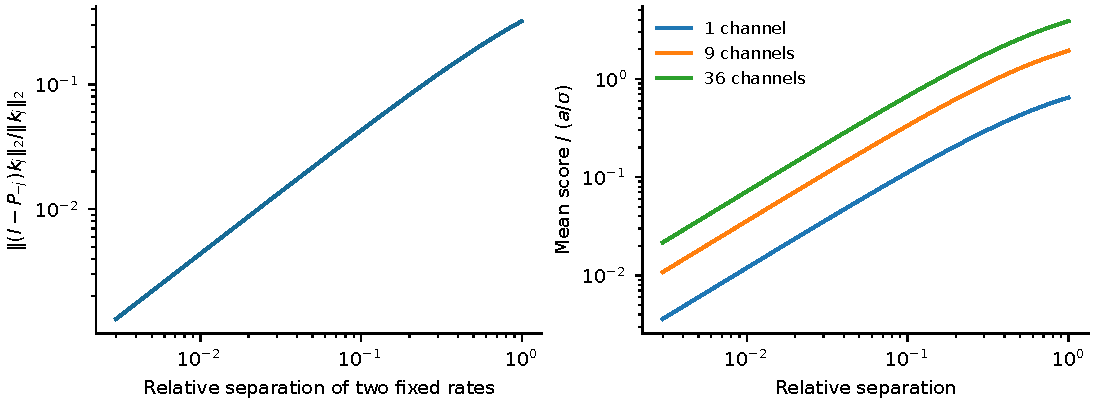
\includegraphics[width=17cm]{figures/geometry.pdf}
\end{adjustwidth}
\caption{Fixed-design illustration of Equation~\eqref{eq:scoremean}, not a reconstruction benchmark. The~two rates are $D/D_0=1$ and $1+\Delta$, with~32 equally spaced $bD_0$ values from 0 to 2.2. Left: the residualized-kernel norm decreases near collision. Right: coherent independent spectral channels increase the expected standardized score by $\sqrt m$ for equal amplitudes. The~rates and groups are fixed in this~calculation.}\label{fig:geometry}

\end{figure}

The operational screen estimates rates from the fitting data and groups spectral channels after a signal mask. Consequently, Proposition~\ref{prop:screen}'s calibration assumptions do not apply to the full estimator. Independent masking alone would not remove all uncertainty: an estimated nuisance kernel can leave a nonzero residualized mean even when the tested component is absent. The~fixed-design result requires correct nuisance rates, or~a separately justified bound on this model error. The~additional null experiments in Appendix~\ref{app:revisionvalidation} assess the operational procedure under their specified generators; they do not replace these assumptions. We use $\alpha=0.01$ as a frozen screening parameter, not as a claimed family-wise error rate or chemical confidence level. If~$\|v_j\|_2<10^{-10}\|k_j\|_2$, the~implementation retains that component's allowed support: numerical nonidentifiability is not evidence of absence. Otherwise an entire group is allowed only when $Z_{jG}$ exceeds the threshold. NNLS still estimates separate nonnegative amplitudes at every retained spectral channel within an allowed~group.

\subsection{Predictive Comparison and Automatic~Order}\label{sec:selection}
The available reconstruction rows are divided into an internal fitting set $T$ and an internal validation set $V$. Candidate paths include orders $0,1,\ldots,4$. For~each path state, both the unrestricted support and, when different, the~screened support are refined on $T$. A~component with no allowed spectral channel is removed before refinement. Write $P_c=\widehat Y_{c,V}=K(b_V,d_c)A_c$ for a candidate's prediction on $V$. Both $P_c$ and $P_{c_*}$ below are predictions; neither is an observed-data residual. Put
\begin{equation}\label{eq:val}
 L_c=\|P_c-Y_V\|_F^2/\sigma^2.
\end{equation}

For numerically eligible candidates, let $c_*$ minimize $L_c$. We retain the set
\begin{equation}\label{eq:selection}
 \mathcal E=\left\{c:L_c\leq L_{c_*}+
 2\|P_c-P_{c_*}\|_F/\sigma+10^{-10}\right\}.
\end{equation}

Within $\mathcal E$, selection is lexicographic: fewer surviving rates, then fewer allowed amplitudes, then lower validation loss. The~selected fixed support is refitted on $T\cup V$. The~zero-signal model is a legitimate candidate. The~selected $r$ is therefore automatic within a declared finite search, without~access to the true order. The~selected order and configured cap are reported. A~selection at that boundary does not establish that no additional rates~exist.

\begin{Proposition}[Conditional paired prediction variance]\label{prop:paired}
Let $P,Q$ be fixed predictions independent of $E$, and~$Y=M+E$ with iid $N(0,\sigma^2)$ errors. Then
\begin{align}
 \mathbb E\{(\|P-Y\|_F^2-\|Q-Y\|_F^2)/\sigma^2\}
 &= (\|P-M\|_F^2-\|Q-M\|_F^2)/\sigma^2,\label{eq:pairedbias}\\
 \operatorname{Var}\{(\|P-Y\|_F^2-\|Q-Y\|_F^2)/\sigma^2\}
 &=4\|P-Q\|_F^2/\sigma^2.\label{eq:pairedvar}
\end{align}
\end{Proposition}
\begin{proof}
Subtracting the losses cancels the quadratic error term. The~random remainder is $-2\langle P-Q,E\rangle/\sigma^2$, a~centered normal variable with the variance in Equation~\eqref{eq:pairedvar}.
\end{proof}

% REVIEW R2.1: distinguish prediction distance and adaptive calibration.
For a fixed pair, define $s(c,d)=2\|P_c-P_d\|_F/\sigma$. Proposition~\ref{prop:paired} gives exactly this standard deviation, rather than a residual-norm approximation, when the pair is independent of validation noise. Equation~\eqref{eq:selection} uses $s(c,c_*)$ as a predictive simplicity allowance. Because~$c_*$ is chosen using the validation losses, the~fixed-pair identity does not calibrate this adaptive decision or supply a simultaneous confidence set. In~particular, the~one-standard deviation multiplier is a declared heuristic; it is not a significance level or a probability that a component is real. Moreover, the~benchmark signal mask uses all outer training rows, some of which become internal validation rows. Conditional independence of predictions and internal validation noise is therefore not exact after masking. The~internal rule is explicitly heuristic. The~eight external test acquisitions remain unused in the mask, candidate fitting, and~selection, preserving an independent predictive evaluation for this full procedure. A~future inferential version would need independent masking or cross-fitting and selection-adjusted calibration; neither has been retroactively attributed to the frozen~benchmark.

The suffix S specifies the complete estimator below: the objective for a fixed $(r,H)$ is Equation~\eqref{eq:nnls}, the~proposal path is native atomic RAI or DOME (Sections~\ref{sec:raiatomic} and \ref{sec:domemath}), and~the final order/support rule is Equation~\eqref{eq:selection}. Screening defines a finite family of constraints; it is not an extra amplitude penalty. In~particular, rates are screened at the native path state before each support-specific refinement. The~screen is not iterated after every rate update. Algorithm~\ref{alg:support} records this order of operations and includes explicit failure~handling.

\begin{algorithm}[H]
\caption{Automatic spectral-support selection for RAI-S and~DOME-S.}\label{alg:support}
\begin{algorithmic}[1]
\Require Observed $(b,Y,\sigma)$, retained spectral channels, diffusion bounds, path method $M$, $r_{\max}=4$.
\Ensure Rates $d$, amplitudes $A$, allowed support $H$, selected order, diagnostics, and~status.
\State Sort distinct $b$; partition supplied rows into fitting $T$ and validation $V$.
\State Form contiguous spectral-channel groups without crossing large chemical shift gaps.
\State $\mathcal P\gets\Call{NativePath}{M,b_T,Y_T,\sigma,r_{\max}}$; include the zero model.
\State $\mathcal C\gets\varnothing$; $\mathcal L\gets\varnothing$ \Comment{Eligible candidates and audit log}
\For{each rate state $d\in\mathcal P$}
  \State $\mathcal H\gets\{\one_{|d|\times p}\}$.
  \If{$|d|>0$}
    \State $H_s\gets\Call{Screen}{b_T,Y_T,\sigma,d,\text{groups},0.01}$ using Equation~\eqref{eq:score}.
    \State Add $H_s$ to $\mathcal H$ if different from the unrestricted support.
  \EndIf
  \For{each $H\in\mathcal H$}
    \State $ (d_H,H)\gets\Call{PruneEmptyRows}{d,H}$.
    \State $c\gets\Call{RefineNNLS}{b_T,Y_T,\sigma,d_H,H}$ using Equations~\eqref{eq:nnls}--\eqref{eq:stationarity}.
    \State Append rates, support type, parameter count, success and KKT to $\mathcal L$.
    \If{$c$ is the zero model, or~solver success, $\eta_z\leq10^{-6}$ and KKT $\leq10^{-7}$}
      \State $P_c\gets K(b_V,d_c)A_c$; $L_c\gets\|P_c-Y_V\|_F^2/\sigma^2$.
      \State Add $(c,P_c,L_c)$ to $\mathcal C$.
    \EndIf
  \EndFor
\EndFor
\If{$\mathcal C=\varnothing$}
  \State \Return unresolved optimization and $\mathcal L$.
\EndIf
\State $c_*\gets\argmin_{c\in\mathcal C}L_c$; construct $\mathcal E$ by Equation~\eqref{eq:selection}.
\State $\widehat c\gets\argmin_{c\in\mathcal E}^{\rm lex}(|d_c|,\ |d_c|+\#\{H_c=1\},\ L_c)$.
\State Refit $(d_{\widehat c},A_{\widehat c})$ on $T\cup V$ with $H_{\widehat c}$ fixed; check diagnostics.
\State Export a mass-conserving 256-bin map; retain final failure or mismatch flags.
\State \Return final $(d,A,H)$, selected order, status, candidate losses, and~$\mathcal L$.
\end{algorithmic}
\end{algorithm}



%\input{sections/experiments}

\section{Reproducible Computational~Study}\label{sec:experiments}

\subsection{Data Partitions and Prespecified Decisions}
The primary study contains 24 development problems and 48 new test problems, generated with disjoint seed ranges beginning at 510,000 and 810,000. A~separate training bank for a neural policy comparison begins at 610,000. A~problem is an entire noisy DOSY matrix, not an individual spectral pixel. The~support configuration was frozen before test evaluation: maximum order four, screening parameter $0.01$, validation stride four, one paired standard deviation allowance, and~at most 350 nonlinear function evaluations per support~refinement.

Support selection gives priority to smaller component order, then to fewer allowed amplitudes (Equation~\eqref{eq:selection}). The screening parameter was not tuned on test data. Appendices~\ref{app:revisionvalidation} and~\ref{app:completevalidation} report additional tests of the prespecified procedure.

Each new problem has 32 acquisition coordinates and 1024 spectral channels uniformly spanning 10 to 0 ppm. In~the primary atomic benchmark, $D_0=10^{-9}\,\mathrm{m^2\,s^{-1}}$ and fitted rates are restricted to $[0.1,15]D_0$. The~native rate constraints in the external comparisons are specified in Appendix~\ref{app:externalcomparison}. The~acquisition design is
\begin{equation}\label{eq:design}
 b_i=10^9 B\left(\frac{i}{31}\right)^\eta\ \mathrm{s\,m^{-2}},
 \quad i=0,\ldots,31,
\end{equation}
with independent $B\sim U(1.3,2.7)$ and $\eta\sim U(1.5,2.4)$. The~component diffusion coefficients are positive and jointly shared across all spectral channels. Their amplitudes have correlated Gaussian spectral peaks, including an overlapping region near 7.73 ppm and other peaks with different mixture proportions. The~exact generator is included with the evidence~package.

\textls[-25]{Eight families contain six problems each: one, two, or~three separated rates; a three-rate weak-component family; a close-rate family; proportional component spectra; noise-only controls; and broad distributions. The~six problems per family use SNR 50, 100, and~200 twice each, with~independently generated parameters and noise. For~positive signals, the~maximum unattenuated spectral intensity is normalized to one in the generator and\linebreak   $\sigma=1/\mathrm{SNR}$. Solvers receive observations in these units, not true \mbox{component~normalizations.}}

Nominal separated rates are $(0.65,2.3,7.1)D_0$, using the first one or two as appropriate, with~independent log-rate perturbations of standard deviation 0.10. Close rates use $(0.8,1.05,5.5)D_0$ with log-rate perturbations of standard deviation 0.02. In~the weak family the third spectrum is multiplied by 0.04 before overall normalization; this is a spectral-amplitude multiplier, not a guarantee of exactly 4\% total mixture mass. In~the proportional family $A_{j\cdot}$ equals $1,0.7,0.45$ times the same spectrum. Broad controls replace each atom by a lognormal distribution with log-width 0.18, using 24-point Gauss--Hermite forward quadrature. The~forward generator uses the lognormal on its full positive domain; its histogram reference is truncated and renormalized on the fitted interval for plotting and shape evaluation. These controls deliberately violate the fitted atomic~model.

Every fourth acquisition, using zero-based indices $i\bmod4=3$, is reserved for external testing. The~remaining 24 rows are available to the reconstruction. A~signal mask thresholds the mean of the first six available low-$b$ rows at $4\sigma/\sqrt6$, followed by \mbox{two one-dimensional} dilation steps. Noise-only controls instead inspect the fixed window $4<\mathrm{ppm}<4.65$. All methods in a comparison receive the same mask. Conditional on that mask, external test noise remains independent. The~reported errors assess retained spectral channels, not undetected parts of a full spectrum; losses caused by masking are not chemical \mbox{absence~certificates.}

After the 24 reconstruction rows are sorted by increasing acquisition coordinate, the~3rd, 7th, 11th, 15th, 19th and 23rd rows form the internal validation set. The~other 18 rows are used for candidate fitting. These are one-based positions within the reconstruction subset, not positions in the original 32-row acquisition. Groups are split where adjacent selected chemical shift spacings exceed 1.6 times their 25th percentile. This rule assumes a substantially regular original spectral grid. It is a segmentation convention, not a learned chemical grouping. The~final selected model uses all 24 reconstruction~rows.

\subsection{Evaluation, Denominators, and~Uncertainty~Summaries}
The primary quantitative panel is the 36 signal-present atomic problems. Six null cases are reported separately because normalized shape and true spectral leakage have no physical denominator there. Six broad cases are misspecification controls. An~additional\linebreak   24-problem archived bank contains finite-width diffusion profiles with one to three generating components, including close and proportional scenarios. It is transfer evidence and is never pooled with the new atomic~bank.

Rates are paired to ground truth by a minimum-cost one-to-one assignment in absolute log distance; pairs beyond $0.25$ are then rejected. ``Order and rates recovered'' requires the correct total order and an accepted pair for every true rate. The~tolerance corresponds to an approximate multiplicative factor of $e^{0.25}$ and~is not a chemical identification standard. On~finite-width controls, matching an atomic rate to a distribution center does not imply recovery of the distribution or a literal~atom.

For each accepted pair $(j,k)$, define an evaluator-only meaningful spectral set\linebreak  
$\mathcal S_k=\{\ell:A^{\mathrm{true}}_{k\ell}>0.001\max_h A^{\mathrm{true}}_{kh}\}$ within the supplied mask. The~leakage \mbox{fraction is}
\begin{equation}\label{eq:leakage}
 \ell_{\mathrm{spec}}=
 \frac{\sum_{(j,k)\ \mathrm{paired}}\sum_{\ell\notin\mathcal S_k}\widehat A_{j\ell}}
 {\sum_{(j,k)\ \mathrm{paired}}\sum_\ell\widehat A_{j\ell}}.
\end{equation}

The implementation assigns zero when its denominator is zero; therefore unmatched estimated mass is always reported alongside it, as~a fraction of all estimated mass. Missing true rates are exposed by the recovery count. The~$0.1\%$ threshold is an evaluation convention and never a fitting cutoff. It is also distinct from the display threshold in the DOSY~figures.

External clean prediction error is $\|\widehat Y_U-Y_U^0\|_F/(\sigma\sqrt{|U|p})$ on the eight unused acquisitions $U$. It measures estimation error without adding a fresh noise variance; observed noisy-test errors are retained in the machine-readable results. Shape loss is $W_1$ in natural-log diffusion, evaluated after exporting both measures to the common 256-cell mass grid, normalizing per positive spectral channel, and~weighting spectral channels by true mass only in the evaluator. A~missing positive estimate receives the declared span penalty $\log150$; it is not described as an actual transport distance. Total estimated mass is saved~separately.

We report problem-level averages with equal weight per problem. The~primary table excludes the null cases; Appendix~\ref{app:legacy} retains the earlier 42-case convention, whose zero contributions dilute shape averages. Bootstrap intervals resample whole paired problems 10,000 times with seed 9925. They are descriptive pointwise intervals for this small heterogeneous simulation bank, not simultaneous tests or calibrated population coverage. Different spectral channels are not treated as independent experimental~replicates.

\subsection{Neural Policy Comparison and Numerical~Verification}
RAI-Net is the action-ranking policy of Section~\ref{sec:rainetmath}, acting on the adaptive distributional objective in Equation~\eqref{eq:raihaar}. It does not directly predict the number of species. Retraining used 80 DOSY problems split by whole problem into 64 training and 16 validation problems, producing 2921 recorded action examples. The~policy has two hidden layers of 48 units with hyperbolic tangent activations. Training lasted 400 epochs and used a transformed noise-standardized internal validation prediction-gain target. The~selected checkpoint was epoch 400, so convergence of learning is not claimed. The~classical objective and numerical acceptance checks remained in~force.

The original and retrained policies were evaluated on the predefined first 24 new test problems and all 24 archived transfer problems. The~new neural panel contains three problems per scenario: 18 signal-present atomic, three null, and~three broad distribution cases. These are smaller panels than the atomic study. The~network results are an auxiliary comparison, not an additional order recovery experiment or evidence for the atomic support~rule.

Numerical verification covers NNLS agreement with an independent implementation, finite-difference checks of the variable-projection Jacobian, coherent weak-signal screening, acquisition partition boundaries, and~amplitude-scaling/spectral channel-permutation behavior. A~direct comparison of the SVD-based active-subset enumerator with an independent Lawson--Hanson active-set NNLS implementation (MATLAB R2026a Update 2) used 100 amplitude columns. Pseudoinverse-based local rate precision, boundary hits, and~a residual-based atomic model warning are exported as diagnostics; none is interpreted as a selection-adjusted confidence interval or goodness-of-fit~test.


\subsection{Validation Studies and Experimental Sampling~Units}\label{sec:extendeddesign}
Table~\ref{tab:revisionunits} identifies the independent inputs and repeated
conditions in each additional study. Methods are compared on the same observations;
additional policies, candidate orders and warm-start budgets do not increase the
number of independent samples. The~supplement contains the configurations, seeds,
checkpoints and failed outcomes. In~the convergence study, we fix the factor count
to examine optimization alone. The~weak-component and experimental studies retain
automatic atomic order~selection.

\begin{table}[H]\small
\caption{Sampling units of the revision studies. Repeated conditions and
methods do not multiply the number of independent inputs.}\label{tab:revisionunits}
\begin{tabularx}{\textwidth}{m{2.5cm}L}\toprule
\textbf{Panel} & \textbf{Independent Input and Repeated Conditions}\\\midrule
Null & 300 noise matrices; 100 per noise scale; paired~methods.\\
Weak & 96 truth/noise matrices; four amplitude factors, three SNRs, eight per~cell.\\
Factorial & 36 existing atomic problems; paired $2\times2$ stages and production~reference.\\
TRAIn-MF & Nine rank--SNR inputs; four warm budgets and two common~starts.\\
Neural & 120 new test problems; five trained seeds and one classical control on~each.\\
External & 47 frozen matrices after one adapter pilot; two stresses on~\linebreak   12 underlying~truths.\\
Experimental & Four resin specimen series with three diffusion-time blocks~each.\\
Public mixture & One 30-acquisition archived experiment; five paired estimators.\\\bottomrule
\end{tabularx}\end{table}

We studied four industrial resin series: TP194-2623086, TP194-2623088,
TP194-2623084 and TP194-2619082. We retain the signed absorption spectra and fit
every channel within the positive support detected from the fitting acquisitions.
Each 23-acquisition block reserves five acquisitions for prediction; neither
these nor the internal validation rows enter support detection. All methods use
the same encoding and support. Coherent negative structure outside the support is
reported and left unestimated. Strong correlation in the processed background
means that its estimated noise scale cannot be interpreted as an iid Gaussian
calibration. We retain the HDO-derived encoding calibration, but~its unquantified
systematic uncertainty prevents assigning a chemical confidence interval.
Appendix~\ref{app:experimentalrevision} describes the samples and the limits of
the available composition~records.


%\input{sections/results}


\section{Results}\label{sec:results}

\subsection{Atomic Recovery and Spectral~Leakage}
Table~\ref{tab:primary} reports the 36 signal-present atomic test problems. RAI-S reduces mean leakage from 5.166\% to 1.728\%, and~DOME-S from 3.857\% to 1.728\%. The~clean external prediction error decreases from 0.2870 to 0.2330 for RAI and from 0.2591 to 0.2330 for DOME. Binned shape loss decreases from 0.1523 to 0.1094 and from 0.1393 to 0.1094, respectively. These are paired changes on the same observations and~masks.



The 
 favorable averages do not hold for every endpoint. Unmatched estimated mass increases from 6.774\% to 7.257\% for RAI and from 7.019\% to 7.257\% for DOME. RAI's correct-order count rises from 17/36 to 25/36, but~DOME's falls from 26/36 to 25/36. The~stricter order-and-rates count improves from 17/36 to 23/36 and from 22/36 to 23/36. Thus, the strongest common conclusion is improved spectral assignment and prediction, not uniformly improved component~counting.


\begin{table}[H]
\caption{New 
 atomic test: 36 signal-present problems, excluding null and broad distribution controls. Leakage and unmatched mass are percentages. $E_U$ is clean external RMSE divided by $\sigma$; $W_{1,h}$ is the binned log-diffusion shape score. A~correct count is weaker than recovery of both order and~rates.}\label{tab:primary}
\begin{adjustwidth}{-\extralength}{0cm}\centering\small
%\input{sections/table_positive}


\begin{tabularx}{\fulllength}{LRRRRRR}\toprule
\textbf{Method} & \textbf{Correct Order} & \textbf{Order and Rates} & \textbf{Leakage} & \textbf{Unmatched Mass} &\boldmath{ $E_U$} &\boldmath{ $W_{1,h}$}\\\midrule
RAI & 17/36 & 17/36 & 5.166 & 6.774 & 0.2870 & 0.1523 \\
RAI-S & 25/36 & 23/36 & 1.728 & 7.257 & 0.2330 & 0.1094 \\
DOME & 26/36 & 22/36 & 3.857 & 7.019 & 0.2591 & 0.1393 \\
DOME-S & 25/36 & 23/36 & 1.728 & 7.257 & 0.2330 & 0.1094 \\
\bottomrule\end{tabularx}

\end{adjustwidth}
\end{table}



For RAI, the~mean leakage change is $-3.438$ percentage points, with~a descriptive 95\% paired bootstrap interval $[-5.282,-1.926]$. For~DOME, the change is $-2.129$ points, with~interval $[-3.155,-1.268]$. The~corresponding clean prediction changes are $-0.0540$ [$-0.0800,-0.0325$] and $-0.0261$ [$-0.0338,-0.0181$]. These intervals summarize the saved 36-case panel under the stated resampling convention; they do not adjust for multiple reported endpoints or establish external experimental~performance.

RAI-S and DOME-S yield effectively identical primary summaries to the displayed precision. Their common post-proposal objective, support rule, and~refinement can erase differences between proposal paths. These outcomes support the shared selection procedure and give no evidence that two independent improvements have been~discovered.

\subsection{Scenario-Level Failures and a DOSY~Illustration}
Figure~\ref{fig:recovery} separates ordinary mixtures from difficult identification regimes. Both screened methods recover order and all rates in all six one-, two-, and~three-separated-component cases. In~close-rate cases, they recover the correct order in 5/6 problems, but~all rates in only 4/6. For~proportional spectra, they recover neither the full three-rate structure nor the correct order in any of six cases. The~original DOME recovers the correct order in one of these cases, so the screened version has a visible~regression.

In the weak family, the~correct order is selected in 2/6 cases, but~the weakest rate is matched in only 1/6; neither original method matches it in these six cases. In~the one matched screened case, approximately 72\% of the true minority spectral mass lies within the retained allowed support. The~support metric is a recall of permitted spectral channels, not a claim of unbiased amplitude recovery. These results leave weak-species detection~unresolved.

\begin{figure}[H]\centering
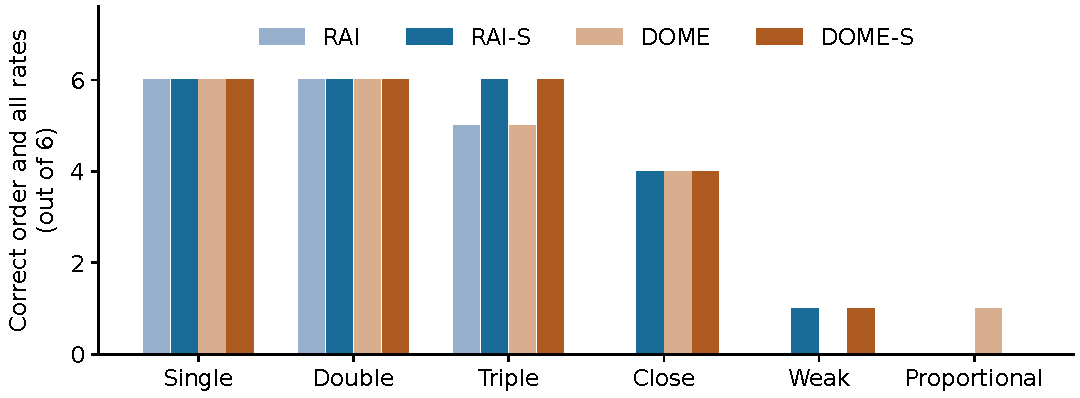
\includegraphics[width=\linewidth]{figures/recovery.pdf}
\caption{Recovery of both order and all rates by scenario in the new atomic test. Every bar has six independently generated problems. Matching uses a log-rate tolerance of 0.25. Narrow output bands and correct order alone do not imply successful~localization.}\label{fig:recovery}
\end{figure}




Figure~\ref{fig:dosyatomic} provides one fixed illustration, rather than selecting a new representative after ranking the test outputs. The~ground truth is displayed explicitly. Correlation is used through common rates and component-specific spectral amplitudes; it is not an assumption that every spectral channel has the same decay. The~color threshold is a plotting convention applied to every panel and has no role in model order or support~estimation.


\begin{figure}[H]

% The preserved source has a clipped vertical color label at its right edge.
% Crop that label only and typeset its exact meaning below; data are unchanged.
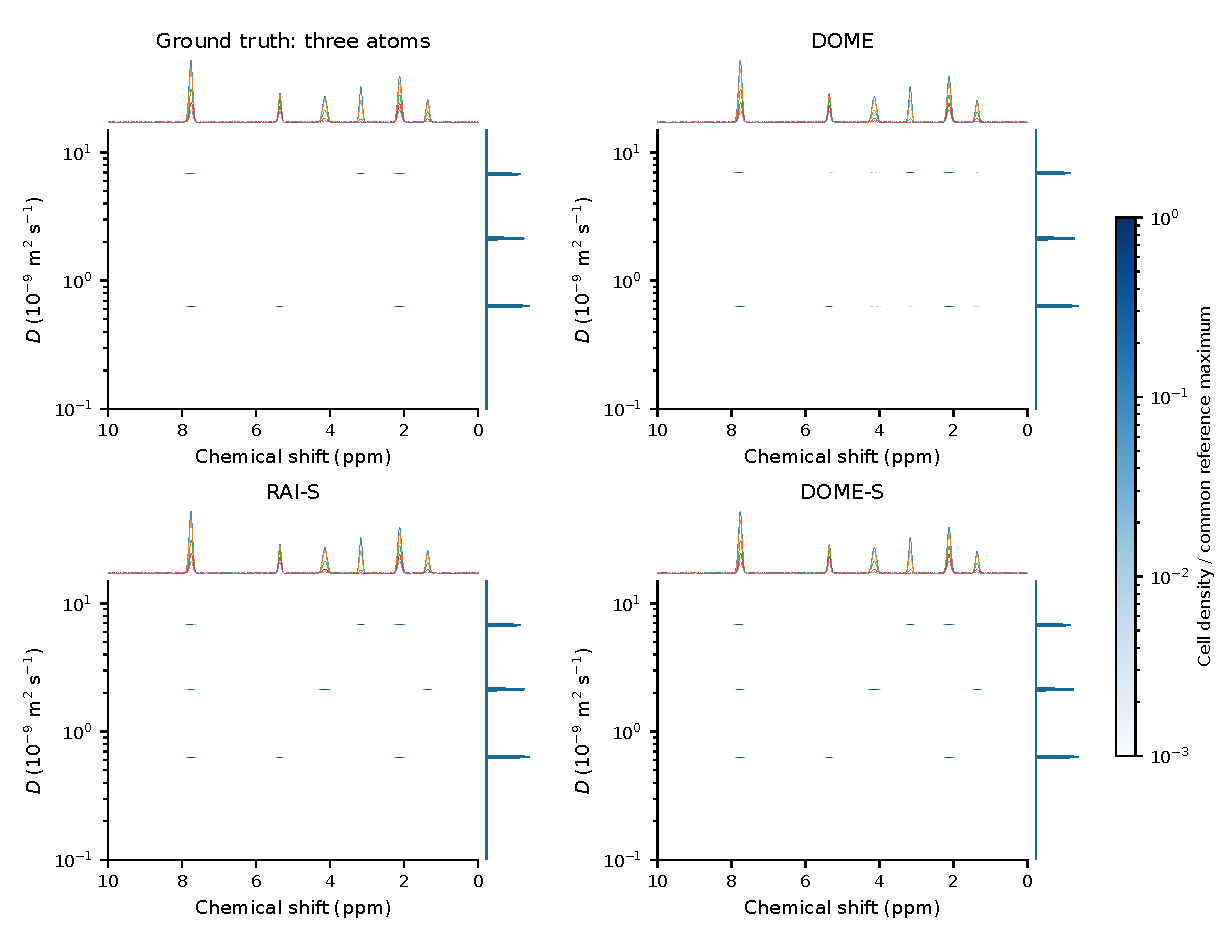
\includegraphics[width=13.2cm]{figures/dosy_discrete.pdf}


\caption{Saved 
 independent test problem 18, with~three true atomic rates and SNR 200. The~complete reference is shown alongside DOME and the two support-selected outputs. All panels use the same selected spectral channels, 256-bin mass-to-density display, and~common absolute reference maximum; values below 0.1\% of that maximum are not colored. The~top traces show measured attenuation spectra. Side projections have separate horizontal scales. The~display creates finite-width cells for atoms; it is not a recovered continuous width. Quantitative results use the unthresholded saved~outputs. Color denotes cell density divided by the common reference maximum on a logarithmic scale; darker blue indicates greater density. White areas lie outside the displayed support or below the stated display floor.}\label{fig:dosyatomic}

\end{figure}


\subsection{Null Controls, Broad Distributions, and~Transfer}\label{7.3}
All four atomic methods select the null model in all six noise-only controls. This observed count is not a guarantee of a population false-positive rate: even under a common Bernoulli model, zero false selections in six trials gives a one-sided 95\% upper bound of $1-0.05^{1/6}=0.393$. The~larger revision controls are reported separately in Appendix~\ref{app:revisionvalidation}, without~pooling them with the frozen study. On~the six broad controls, the~screened methods have clean prediction error 0.2382, compared with 0.3664 for RAI and 0.2837 for DOME. Their binned shape score is 0.1638, compared with 0.2686 and 0.1972. An~atom model nevertheless cannot reproduce nonzero distributional width exactly. The~apparent improvement in prediction is therefore not evidence of recovered width. For~a positive diffusion measure with mass $M$, mean $\bar D$, variance $v$ and support $D\geq D_{\min}\geq0$, convexity and Taylor's theorem give the finite-measurement bound
\[
0\leq\int e^{-bD}\,d\mu(D)-M e^{-b\bar D}\leq \tfrac12 M b^2 e^{-bD_{\min}}v.
\]

Thus, a narrow continuous profile can have an attenuation close to an atomic one on the sampled interval. Reducing the allowed spectral support can trade approximation bias against estimation variance. This explains why lower prediction error is compatible with an incorrect measure class; it is not a proof that variance reduction alone caused the observed improvement or that the true distributional width was identified. Counting its fitted rates against the number of generating broad profiles is a descriptive center-count comparison, not a valid literal atom-recovery~claim.

On the 24 archived finite-width problems, leakage decreases from 1.245\% to 0.082\% for both native paths. Clean prediction error changes from 0.2650 to 0.2329 for RAI and from 0.2492 to 0.2329 for DOME. The~selected-order count agrees with the number of generating profiles in 19/24 screened fits versus 18/24 native fits, while the stricter matching count remains 18/24. Transfer performance is encouraging for spectral assignment, but~the differing true measure class prevents pooling it with the atomic~test.



Figure~\ref{fig:dosycontinuous} retains the existing TRAIn-MF reconstruction and its native grid. For~this case, the~native atomic leakage of approximately 1.975\% decreases to 0.279\% after support selection, with~three selected rates. The~TRAIn-MF result is used to display the distinction between distributional factorization and atomic inference. It was not recomputed for this manuscript, and~the figure is not a new all-method performance ranking. No conclusion about polymer molecular weights is drawn without a separate calibration and experimental~analysis.

\begin{figure}[H]

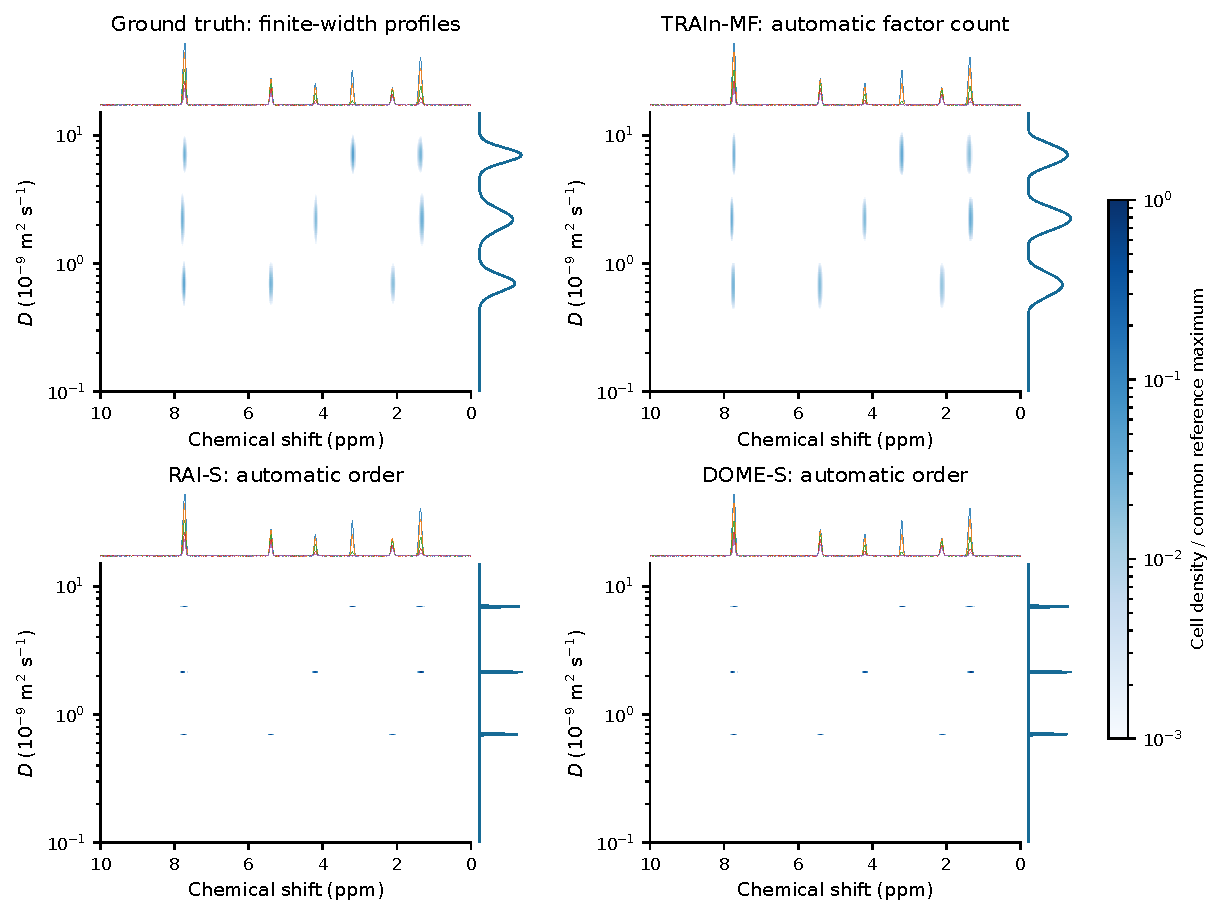
\includegraphics[width=13.2cm]{figures/dosy_continuous.pdf}

\caption{Archived 
 three-component problem at SNR 200 (replicate 1): three finite-width lognormal diffusion profiles, SNR 200, and~120 selected spectral channels of 1024. Ground truth, the~unchanged automatic TRAIn-MF reference, RAI-S, and~DOME-S are shown. TRAIn-MF uses its original masses and original cell edges without remapping. Its factor count and the atomic methods' order are selected automatically but have different meanings. The~common reference maximum is 63.34986357 in the saved cell-density units, with~a 0.1\% display floor. Side projections are separately scaled. Fitted atoms occupy individual export cells and do not estimate the true~widths. Color denotes cell density divided by the common reference maximum on a logarithmic scale; darker blue indicates greater density. White areas lie outside the displayed support or below the stated display floor. The colored top traces correspond to individual acquisitions.}\label{fig:dosycontinuous}

\end{figure}



\subsection{Exploratory Neural Policy~Comparison}
Table~\ref{tab:net} reports the policy comparison. On~24 new test problems, the relative change in mean binned shape score is approximately 0.041\%, with~mean paired difference $-0.000111$ and bootstrap interval $[-0.001356,0.001105]$. The~clean-error interval also includes zero. On~the archived transfer panel, the~shape score improves by approximately 1.48\%, but~this does not establish an advantage on the new test. One fit per policy in the archived panel fails its numerical convergence criterion; both outputs remain in the reported~averages.

\begin{table}[H]
\caption{RAI-Net 
 policy comparison on its predefined panels. These are distributional methods, so no chemical order recovery count is assigned. All saved outcomes, including the two numerical failures, enter the~averages.}\label{tab:net}
 
\begin{adjustwidth}{-\extralength}{0cm}
%\centering %% If there is a figure in wide page, please release command \centering


\begin{tabularx}{\fulllength}{LLRRR}\toprule
\textbf{Panel} & \textbf{Policy} & \boldmath{$W_{1,h}$} & \boldmath{$E_U$} & \textbf{Numerical Success}\\\midrule
New test, $n=24$ & Original & 0.272268 & 0.307991 & 24/24\\
 & Retrained & 0.272157 & 0.307921 & 24/24\\
Archived, $n=24$ & Original & 0.204769 & 0.326401 & 23/24\\
 & Retrained & 0.201739 & 0.326324 & 23/24\\\bottomrule
\end{tabularx}
\end{adjustwidth}
\end{table}

The new neural panel includes atomic, broad, and~null cases, with~zero shape-score contributions for nulls under the archived bookkeeping convention. Its averages therefore do not share the population of Table~\ref{tab:primary}. The~policy ranks adaptive actions within an existing numerical procedure. It neither adds observations nor certifies the chemical support. These data do not support promoting the retrained policy as a superior substitute for the support-selected atomic estimator, and~the two are not compared as if they shared the same output class. This small exploratory comparison is inconclusive. A separate experiment uses five reproducible training seeds and 120 new whole-problem tests, including noise and acquisition-design shifts, against~a classical policy with the same search caps (Appendix~\ref{app:neuralexpanded}). Numerical failures, realized costs and paired whole-problem intervals are reported there; the extended experiment is not pooled with Table~\ref{tab:net}.


\subsection{Extended Computational and Experimental~Validation}\label{sec:extendedresults}
The factorial experiment in Appendix~\ref{app:completevalidation} examines
screening and predictive selection separately. For~RAI, screening at native order
reduces clean error from 0.30677 to\linebreak   0.29087 noise units. Predictive selection alone
gives 0.26189, and~combining the stages gives 0.23145. DOME reaches the same final
factorial result from a different native-order baseline. These interventions
support a contribution from both shared stages on this panel, with~an interaction,
without demonstrating an independent advantage of either proposal family. Unlike
the mandatory-screening factorial arm, the~production selector also considers
unrestricted support and reproduces the original saved~result.

In the larger weak-component panel, RAI-S matches the minority rate in 45/96 fits
and DOME-S in 44/96. Figure~\ref{fig:weakpowerrevision} shows how recovery changes
with SNR and amplitude. Even though all fits meet their numerical criteria, the~
smallest components are often missed; a nonselected component cannot generally be
declared absent. The~TRAIn-MF study in Appendix~\ref{app:mfconvergence} also shows
why iteration counts need a separate stationarity check. Only 14 of 36 selected
fits meet the $10^{-6}$ KKT tolerance within the common SQP budget. We retain the
22 unresolved fits in the objective and prediction~summaries.

All 720 final outputs in the larger neural study pass their numerical checks.
After averaging the five neural metrics within each problem, the~difference
from the classical shortlist is $\Delta W_{1,h}=-0.00054$, with~a descriptive
95\% interval $[-0.00174,0.00056]$ over 105 signal-present problems. The~clean-error
difference is $-0.00012$, with~interval $[-0.00044,0.00010]$ over all 120 problems.
Both intervals include zero, so the study does not establish improved accuracy.
The neural policies require fewer fixed-tree fits under the same search caps;
Appendix~\ref{app:neuralexpanded} gives the cost definitions and accounts for the
reused training~traces.

Table~\ref{tab:externalexecuted} compares the attributed implementations of SCORE and LOCODOSY, a positive-amplitude SCORE variant, and positive distributional controls. All methods predict the same withheld observations, but~their component
counts and distributional shape scores have different meanings. Every returned
estimate enters the prediction summary; numerical failures and outputs that do
not define a positive measure are identified separately. This is a comparison of
the stated implementations and tuning policies, rather than a universal ranking
of algorithm~names.

The industrial resin study in Appendix~\ref{app:experimentalrevision} tests the
methods on measured spectra with processing distortions and strongly correlated
background. Here, the~fitted atomic order describes a model of the data; reaching
the search cap does not identify the number of constituents. A~signed fit can
have a smaller predictive error while relying on nearly coincident rates and
canceling spectra. These experimental outcomes test the scope of the synthetic
conclusions and retain model mismatch and optimization~flags.

The public 30-acquisition example in Appendix~\ref{app:publicmixture} provides
a useful counterexample. Its archived sample text documents propanol and sucrose.
All four final global fits and all\linebreak   27 local SCORE solver calls pass their numerical
checks, yet signed SCORE predicts best: test NRMSE is $0.232\%$, compared with
$0.582\%$ for RAI-S and DOME-S and $0.270\%$ for LOCODOSY. The~signed SCORE fit
also passes the conditioning checks, so its advantage cannot be attributed to
failed optimization. Amplitude constraints and possible acquisition-model error
affect this comparison. RAI-S and DOME-S reach the cap and flag model mismatch.
We therefore find no general experimental predictive advantage for the positive
global selector. The~nominal solutes do not establish the full composition,
chemical assignments or independently measured diffusion~coefficients.

\subsection{Numerical Diagnostics}
Across 144 support-selected fits in the primary and transfer panels, the maximum relative amplitude KKT residual was $1.12\times10^{-15}$ and the maximum normalized projected log-rate residual was $1.34\times10^{-7}$. Four poor-precision flags and four atomic model-mismatch flags were recorded. In the independent 100-column NNLS comparison, the relative prediction discrepancy was $4.62\times10^{-17}$. All native and support-selected atomic fits in these panels met their numerical stopping criteria. The two neural failures occurred on the same problem. Appendix~\ref{app:completevalidation} gives separate numerical failure counts for the additional studies. A small stationarity residual does not establish precise rates or chemical identification.



%\input{sections/discussion}



\FloatBarrier
\section{Discussion}
Our formulation makes clear which part of the result comes from the representation,
the regularization, the~optimizer and the available information. Exporting a fit
on 256 bins reduces display quantization; it does not create 256 independent
diffusion observations. Likewise, a~lower prediction error cannot by itself
identify distributional width, chemical species or a unique~factorization.

The support selector limits the assignment of a proposed rate to unrelated
spectral regions. It first asks whether that rate contributes beyond the other
candidate decays, using groups of channels to retain coherent weak signals.
Unrestricted support remains a candidate. The~factorial study finds contributions
from both screening and predictive selection, together with an interaction.
It does not establish an independent advantage for the RAI or DOME proposals.
Their primary outputs coincide, as~do many of the additional outputs, although~
the weak-component panel contains one different minority-rate match. The~searches
have not been proved~equivalent.

The spectral groups are geometric windows and need not coincide with chemical
resonances. Masking can remove weak signal, errors in nuisance rates can bias the
residualized score, and~nearly coincident rates make its direction ill-conditioned.
Proposition~\ref{prop:screen} and the stability bounds describe fixed designs.
The 300 null matrices and 96 weak-component problems characterize particular
generators; they do not calibrate $\alpha=0.01$ as a universal family-wise error
rate. The~prediction allowance uses the correct difference between fitted
predictions, but~choosing the best model and searching supports make its subsequent
use heuristic. The~discovery masks in the new weak-component and experimental
studies exclude validation observations. This removes one source of data reuse,
while leaving uncertainty in the estimated nuisance model and the need for
selection-adjusted~inference.

A TRAIn-MF factor represents a shared distribution, which may be broad or
multimodal. Its unit-mass normalization fixes scale, not chemical identity.
The runtime curvature check concerns injectivity of a conditional subproblem.
The controlled warm-start study supplies factor count to isolate optimization
and records nonstationary outcomes. It therefore tests neither automatic species
selection nor convergence to a global minimum. The~search caps and iteration
budgets remain essential parts of the reported~procedure.

An atomic model can predict the measured attenuation of a broad distribution
well because the Laplace operator smooths differences between measures.
The bound in Section~\ref{7.3} explains why good prediction can coexist with an
incorrect distributional model. Screening may reduce estimation variance at
the cost of approximation bias, but~the prediction gains alone do not isolate
that mechanism or recover the true width. This matters for industrial resins,
whose heterogeneity may require more than a few atoms. Their selected model
order should not be read as a count of molecular~constituents.

The external comparisons show how strongly the result depends on the fitted
representation and the chosen evaluation measure. Signed cancellation, native
order rules and incomplete optimization remain visible alongside prediction
error. A~signed fit may not define a positive measure, so transport scores
computed only on eligible outputs describe different subsets. On~the public
mixture, signed SCORE converges and passes the stability checks; it and LOCODOSY
predict better than the positive global estimators. We report that advantage
without treating it as proof of chemical recovery. The~nominal composition
provides neither a complete reference order nor independently measured diffusion
coefficients. These results also cannot rank the four external methods that
were not~run.

The larger neural study compares five seeded policies on 120 new problems,
including changes in noise and acquisition design. All policies use the same
search caps and numerical acceptance checks. The~policies share a trace bank
and test problems; their 720 fitted outputs are not 720 independent mixtures.
We average seed-level metrics within each problem before the paired analysis
and retain numerical failures. The~pooled accuracy intervals include zero. The~cost
reduction is conditional on the stated training and search design and does
not establish an end-to-end speedup or experimental chemical~recovery.

The resin measurements provide four specimen series, each with three
diffusion-time blocks. They do not provide twelve independently prepared
mixtures of known composition. Their strongly correlated background and possible
phase, baseline, suppression, exchange, relaxation or encoding errors can violate
the ideal observation model. Support is detected without the reserved acquisitions;
negative coherent structure and unestimated regions remain documented.
Prediction on reserved acquisitions and consistency across diffusion times are
useful checks, but~neither supplies a component diffusion reference or a
molecular-weight calibration. The~experimental interpretation must remain within
those~limits.

\section{Conclusions}
Joint positive Laplace inversion can improve spectral assignment when shared
components are supported by the data. The~distinction between bin masses,
densities, atoms and shared profiles is essential to interpreting the result.
Our conditional stability and uniqueness calculations explain where reconstruction
can fail; the additional experiments show those limits in practice. Weak rates
are missed, finite optimization budgets leave some fits nonstationary, and~the
neural accuracy gains remain inconclusive. The~observed reduction in spectral
leakage therefore supports a specific empirical contribution. Chemical identity
and distributional width require additional~evidence.


%\input{sections/backmatter}

\supplementary{The following supporting information is available at \linksupplementary{s1}: Supplementary File S1, \emph{Computational protocols and data}. It contains the study designs, numerical settings, model outputs, trained neural policies and processed experimental inputs used in the comparisons.}
%\section*{Supplementary Materials}




\authorcontributions{Conceptualization, I.F. and F.M.A.-C.; methodology, V.V., M.G.-L., I.F. and F.M.A.-C.; software, V.V. and F.M.A.-C.; validation, V.V., M.G.-L., I.F. and F.M.A.-C.; formal analysis, V.V. and F.M.A.-C.; investigation and data curation, V.V. and M.G.-L.; writing---original draft preparation, V.V. and F.M.A.-C.; writing---review and editing, V.V., M.G.-L., I.F. and F.M.A.-C.; visualization, V.V. and F.M.A.-C.; supervision, I.F. and F.M.A.-C.; project administration, F.M.A.-C. All authors have read and agreed to the submitted version of the~manuscript.}

%\section*{Author Contributions}


\funding{This research has been funded by the State Research Agency of the Spanish Ministry of Science and Innovation (PID2021-126445OB-I00), and~by the Gobierno de Espa\~na MCIN/AEI/10.13039/\linebreak  501100011033 and Uni\'on Europea ``Next Generation EU''/PRTR (PDC2021-121248-I00, PLEC2021-007774 and CPP2022-009967).}

%\section*{Funding}




\institutionalreview{Not applicable. This study used numerical simulations and NMR measurements of nonbiological materials; it involved no human participants or animal experiments.}

\informedconsent{Not applicable. No human participants were involved in this study.}


%\section*{Institutional Review Board Statement}
%Not applicable to the computational experiments and diffusion spectra of nonbiological industrial resins and public reference mixtures reported~here.
%
%\section*{Informed Consent Statement}
%Not applicable to the computational experiments and diffusion spectra of nonbiological industrial resins and public reference mixtures reported~here.




\dataavailability{The method implementations, synthetic benchmark generators and public validation summaries are available in the TRAIn-DOSY repository at \url{https://github.com/fmarrabal/train-dosy} (accessed on 9 November 2026)~\cite{software}. The processed industrial resin spectra and fitted amplitudes are supplied in Supplementary File S1 and are not distributed in the public repository. The public DOSY mixture is available from the Manchester NMR Methodology Group~\cite{dosytoolboxdata}; its preprocessing and acquisition partitions are documented in File S1.}


\acknowledgments{We 
 used Codex to assist with programming the TRAIn-DOSY repository and Trinka
to improve the manuscript text. The~authors take responsibility for the software,
analyses and manuscript~content.}


\conflictsofinterest{The authors declare no conflicts of~interest.} 

%\section*{Conflicts of Interest}
%The authors declare no conflict of~interest.
%
%\section*{Declaration of Generative AI and Language Assistance}
%We used Codex to assist with programming the TRAIn-DOSY repository and Trinka
%to improve the manuscript text. The~authors take responsibility for the software,
%analyses and manuscript~content.



\appendixtitles{yes}
\appendixstart
\appendix
\renewcommand{\theHequation}{appendix.\arabic{equation}}
\renewcommand{\theHproposition}{appendix.\arabic{proposition}}
%\input{sections/appendix}


\section{Further Mathematical and Numerical~Details}

\subsection{Scaling and~Invariance}
In the atomic model, replacing $(Y,\sigma)$ by $(cY,c\sigma)$ for $c>0$ maps $A$ to $cA$, leaves rates fixed, and~preserves the normalized objective and screening scores. The~same transformation preserves the paired allowance in Equation~\eqref{eq:selection}. Thus, for~unchanged candidate paths and masks, the~exact-arithmetic decision is invariant to signal units. Finite solver tolerances and tie handling can introduce small numerical differences. Changing physical diffusion units with the reciprocal change in $b$ also preserves $bD$ and the predictions. Rescaling observations without rescaling $\sigma$ changes the statistical~problem.

The TRAIn-MF objective has a related property through $\widetilde Y=Y/s_Y$: multiplying the data by $c$ changes $s_Y$ by $c$, leaves normalized factors unchanged, and~rescales the exported amplitudes. Changing the number of spectral channels is different. Averaging the data term by $p$ and the amplitude penalty by $p$ does not make arbitrary deletion of spectral channels innocuous; the available shared information changes. The~exact grid, quadrature, and~regularization operator must also be kept fixed when claiming numerical equality of two TRAIn-MF~outputs.

\subsection{A Local Separation~Expansion}
For the split in Equation~\eqref{eq:split}, write $\delta_1=-(1-\pi)\Delta$, $\delta_2=\pi\Delta$. Taylor expansion of $e^{-t(m+\delta)}$ in the dimensionless coordinates of Section~\ref{sec:domemath} gives a first-order term proportional to $\pi\delta_1+(1-\pi)\delta_2=0$, and~a second-order term proportional to \mbox{$\pi\delta_1^2+(1-\pi)\delta_2^2=\pi(1-\pi)\Delta^2$.} The~bounded-interval remainder is $O(\Delta^3)$ for a fixed finite acquisition design. The~derivative in $\Delta$ vanishes at collision; a variance parameter can expose a nonzero second-order direction. This changes search geometry, not the measured information. After~NNLS and rate refinement, moment preservation of the proposal is not a constraint on the final~estimate.

\subsection{Support Geometry and Precision~Warnings}
For an interior fixed active set, the~first-order rate information after treating amplitudes as nuisance involves projected kernel derivatives, weighted by amplitudes across spectral channels. Extra rows or differently weighted spectra can add information. In~proportional spectra, repeated columns may reduce variance by replication, while preserving the same decay-mixture proportions. If~all relevant projected derivatives vanish, local rate separation fails irrespective of the plotted bin~count.

The software additionally records the condition of the full residual Jacobian and the diagonal of a pseudoinverse of its Gram matrix. Residual-dependent terms, singular directions, active-set changes, and~model selection prevent interpreting this output as a calibrated Fisher-information confidence interval. In~particular, a~pseudoinverse can return finite entries even when some directions are unidentifiable. The~separate condition warning must be retained. A~small normalized projected gradient establishes neither small parameter error nor precise component~identification.

\section{Effect of Including Null Controls in Shape Metrics}\label{app:legacy}
Table~\ref{tab:legacy} averages over 42 atomic problems, including six null cases assigned zero leakage and shape error by convention. Including these zeros lowers the average without changing any reconstruction. The primary analysis therefore reports shape scores for the 36 signal-present problems and reports null selection separately.
\begin{table}[H]
\caption{Earlier 
 42-case convention, including six null controls. Columns are defined as in \mbox{Table~\ref{tab:primary}.} The~zero-valued null shape contributions are bookkeeping conventions, not normalized Wasserstein~distances.}\label{tab:legacy}
\begin{adjustwidth}{-\extralength}{0cm}\centering\small
%\input{sections/table_legacy42}


\begin{tabularx}{\fulllength}{LRRRRRR}\toprule
\textbf{Method} & \textbf{Correct Order }& \textbf{Order and Rates} & \textbf{Leakage} & \textbf{Unmatched Mass} & \boldmath{$E_U$} & \boldmath{$W_{1,h}$}\\\midrule
RAI & 23/42 & 23/42 & 4.428 & 5.806 & 0.2460 & 0.1306 \\
RAI-S & 31/42 & 29/42 & 1.481 & 6.220 & 0.1997 & 0.0938 \\
DOME & 32/42 & 28/42 & 3.306 & 6.016 & 0.2221 & 0.1194 \\
DOME-S & 31/42 & 29/42 & 1.481 & 6.220 & 0.1997 & 0.0938 \\
\bottomrule\end{tabularx}

\end{adjustwidth}
\end{table}


\section{Computational Reproducibility}\label{app:repro}
The joint atomic reconstructions were implemented in Python. TRAIn-MF was run in MATLAB R2026a Update 2 with Optimization Toolbox 26.1. The public repository~\cite{software} provides the synthetic data generators, acquisition partitions, model settings and evaluation code. Supplementary File S1 gives the study-specific protocols and processed experimental inputs. The primary DOSY figures use the fitted profiles or atomic amplitudes from the reported experiments; drawing these maps does not require estimating the models again.

The five RAI-Net policies were trained on CPU. File S1 specifies the training and test problems, the fitted neural policies and the corresponding classical control. Unresolved numerical fits are included in the reported results.


%\input{sections/method_details}


\section{Additional Inversion Models}\label{app:extensions}

\subsection{The Density-RAI~Graph}\label{app:graphdetails}
For column $\ell$, let $a_\ell=\max_i|y_{i\ell}|$, $v_{i\ell}=y_{i\ell}/a_\ell$, and~$s_{i\ell}=\sigma_{i\ell}/a_\ell$, with~a positive numerical floor on $a_\ell$. For~two columns meeting the SNR requirement, the~inspected density implementation uses
\begin{equation}\label{eq:graphdistance}
 d_{\ell m}=\frac1n\sum_i
 \frac{(v_{i\ell}-v_{im})^2}
 {s_{i\ell}^2+s_{im}^2+v_{i\ell}^2\max_k s_{k\ell}^2+v_{im}^2\max_k s_{km}^2}.
\end{equation}

An edge is admitted only below the fixed distance threshold and when both columns include the other among their nearest eligible neighbors; ties at the neighbor cutoff are retained. Then $W_{\ell m}=e^{-d_{\ell m}}$. The~denominator accounts heuristically for uncertainty in shape normalization, but~Equation~\eqref{eq:graphdistance} is not a calibrated test statistic. Estimating this graph from the available fitting rows changes the estimator; fixed-graph convexity applies conditionally after that~construction.

\subsection{A Feasible Primal--Dual Gap for Adaptive Haar~RAI}\label{app:haargap}
Use the notation of Equation~\eqref{eq:raiadmm}, and~let $\mathcal P(Z)=\lambda\sqrt p\sum_{h\geq2}\|Z_{h,:}\|_2$. Choose $N\leq0$ entrywise and a matrix $D$ with first row zero and $\|D_{h,:}\|_2\leq\lambda\sqrt p$ for detail rows. These are dual-feasible for the nonnegative cone and Haar penalty, respectively.
Let\linebreak   $u_\ell^*=H_\ell^{-1}(c_\ell-N_\ell-Q^\top D_\ell)$. Then
\begin{equation}\label{eq:haargap}
 \mathcal G(U,N,D)=\frac12\sum_\ell\|U_\ell-u_\ell^*\|_{H_\ell}^2
 +\mathcal P(QU)-\langle D,QU\rangle-\langle N,U\rangle.
\end{equation}

For $U\geq0$, every term is nonnegative, and~completing the quadratic square shows that $\mathcal G$ equals a primal value minus the corresponding feasible dual lower bound. It therefore bounds suboptimality on this fixed tree. In~ADMM the code uses the feasible primal iterate $V$, projects $\rho d_V$ to the nonpositive orthant, and~projects $\rho d_Z$ to the row balls above. For~the separate penalty, the balls become entrywise intervals $[-\lambda,\lambda]$. At~$\lambda=0$, it uses $N=\min(-\nabla f(U),0)$ and $D=0$ after ridge NNLS. Floating-point gap values are floored at zero to remove negative roundoff; this is a numerical bound construction, not interval~arithmetic.

For completeness, let $m_{j\ell}$ be the current mass in leaf $j$, $\bar k_j$ its unit-mass kernel, and~$w_j$ its log width. At~each spectral channel, the nuisance matrix concatenates columns $m_{j\ell}\bar k_j$ and $(m_{j\ell}w_j/2)\partial_x k(x_j)$ for occupied leaves, divided by that spectral channel's noise. Occupied means $m_{j\ell}>\max(0.02\max_hm_{h\ell},\operatorname{median}_i\sigma_{i\ell})$. Its left singular vectors with singular value at least one form $U_{\rm vis}$. For~a prospective split contrast $t_j=(\bar k_{j,L}-\bar k_{j,R})/2$, put
\begin{equation}\label{eq:haarscore}
 v_{j\ell}=(I-U_{\rm vis}U_{\rm vis}^\top)(t_j/\Sigma_\ell),\quad
 s_{j\ell}=\frac{\langle v_{j\ell},(Y-B_{\rm fine}C)_\ell/\Sigma_\ell\rangle^2}
 {\|v_{j\ell}\|_2^2},\quad I_{j\ell}=m_{j\ell}\|v_{j\ell}\|_2.
\end{equation}

The score is set to zero if the denominator is at most $10^{-24}$ or $I_{j\ell}<0.05$. A~raw score $s^0_{j\ell}$ omits nuisance projection. Joint-detail proposals rank leaves by $\sum_\ell s_{j\ell}$, private-detail proposals by $\max_\ell s_{j\ell}$, position proposals by $\sum_\ell s^0_{j\ell}$, and~occupied-region proposals by $w_j\max_\ell m_{j\ell}$. At~most four leaves are split per action, subject to capacity. The~sibling pair with the smallest difference in its regional mass vectors supplies a merge proposal. These are deterministic heuristics inside the finite tree search, not tests of chemical~identity.

\subsection{The 14 RAI-Net Action~Features}\label{app:netfeatures}
For an action affecting leaves $I$, current leaf count $m$, candidate count $m'$, and~fine count $q$, the~feature vector used in Equation~\eqref{eq:rainet}, in~stored order, is
\begin{align}\label{eq:netfeatures}
 \phi_a=\big(&m/q,\ m'/q,\ \one_{\rm merge},\ \one_{\rm position\ or\ occupied},\nonumber\\
 &\log(1+\textstyle\sum_{j\in I,\ell}s_{j\ell}),\
 \log(1+\max_{j\in I,\ell}s_{j\ell}),\
 \log(1+\textstyle\sum_{j\in I,\ell}s^0_{j\ell}),\nonumber\\
 &\log(1+\max_{j\in I,\ell}I_{j\ell}),\
 \frac{\sum_{j\in I,\ell}m_{j\ell}}{\max(\sum_{j,\ell}m_{j\ell},10^{-300})},\
 \frac{|I|^{-1}\sum_{j\in I}w_j}{\sum_jw_j},\nonumber\\
 &\log(1+\lambda),\ \log(1+n_{\rm supplied}),\ \log(1+p),\ \log(1+F_{\rm current})\big).
\end{align}

The acquisition-count feature is the number of supplied reconstruction rows before the internal split, not an external-test count. The~action scorer sees the state derived from fitting rows; validation is used separately to train the revised priority target and to select completed penalty paths. Networks and checkpoints are therefore tied to the feature semantics as well as their matrix~dimensions.

\subsection{DOME Support~Averaging}\label{app:domeaverage}
The historical averaging variant holds the rates selected by native DOME fixed. At~each spectral channel it enumerates subsets $J$ of these rates, including the empty subset, and~computes NNLS amplitudes $a^{J}_\ell$ and $c_{J\ell}=\mathrm{RSS}_{J\ell}/\sigma^2+6|J|$. The~penalty counts the nominal subset size even if some fitted amplitudes are zero. With~temperature $T=0.5$, it solves the finite entropy-regularized averaging problem
\begin{equation}\label{eq:domeaverage}
 \min_{w\geq0,\,\sum_Jw_J=1}\sum_Jw_Jc_{J\ell}+T\sum_Jw_J\log w_J,
 \quad w_{J\ell}=\frac{e^{-c_{J\ell}/T}}{\sum_Le^{-c_{L\ell}/T}},\quad
 \bar a_\ell=\sum_Jw_{J\ell}a^J_\ell.
\end{equation}

\textls[-15]{Soft weights can retain weak contributions; they are not posterior probabilities or confidence levels. The~rate set is not re-estimated, and~single-channel inputs bypass this averaging. This construction is mathematically different from DOME-S, which screens allowed supports, refines rates for each candidate, and~selects by reserved-acquisition~prediction.}

\subsection{RAI-FLEX: Joint Atomic and Smooth~Profiles}\label{app:raiflex}
RAI-FLEX uses $r_a$ atoms and $r_c$ shared smooth profiles. Let $\varphi_h$ be 24 nonnegative, unit-integral cubic B-splines in log diffusion, $G$ their integrated Laplace matrix, and~$L_2$ their second-derivative quadrature operator. The~predicted matrix is $H(d,C)A$ with\linebreak   $H(d,C)=[K(d),GC]$. The~objective is
\begin{equation}\label{eq:raiflex}
 \min_{d,\,C\geq0,\,\one^\top C=\one^\top,\,A\geq0}
 \tfrac12\|(H(d,C)A-Y)/\Sigma\|_F^2+\tfrac\lambda2\|L_2C\|_F^2,
 \quad \lambda=0.01.
\end{equation}

Rates satisfy the physical bounds. NNLS eliminates $A$ at every evaluation. Initial optimization uses log rates and columnwise $C=\operatorname{softmax}(Z)$ with bounded logits, followed by direct simplex refinement to reach boundary profiles that a softmax gradient can represent poorly. The~profile gradient is
\begin{equation}\label{eq:flexgrad}
 G_C=G^\top((HA-Y)/\Sigma^2)A_c^\top+\lambda L_2^\top L_2C,
 \qquad G_{Z,j}=C_j\odot\{G_{C,j}-(C_j^\top G_{C,j})\one\}.
\end{equation}

Here $A_c$ denotes the continuous-profile rows. A~small logit gradient alone need not imply a small simplex KKT residual. After~L-BFGS-B, up~to 40 refinement sweeps alternate convex simplex quadratic profile updates, bounded atomic log-rate updates, and~NNLS amplitudes, recording a scaled KKT residual with threshold $10^{-6}$.

The archived comparison searches allocations $r_a+r_c=r$ for $r=1,\ldots,4$; the general software default has a larger cap. There is no zero-model candidate in this RAI-FLEX search. A~local effective dimension projects profile/rate tangent directions away from active spectral-amplitude directions. If~$T_\perp$ is this weighted tangent matrix and $P$ the tangent penalty Hessian, the~count is
\begin{equation}\label{eq:flexdf}
 d_{\rm eff}=d_A+\tr\{(T_\perp^\top T_\perp+P)^+
                                      T_\perp^\top T_\perp\}.
\end{equation}

Here, $d_A=\sum_\ell\rank(\diag(\Sigma_\ell^{-1})H_{J_\ell})$ for the active amplitude subsets $J_\ell$; density tangent contrasts use spline coefficients above $10^{-5}$. The~pseudoinverse is numerically truncated. The~selector minimizes $\mathrm{RSS}/\sigma^2+2d_{\rm eff}+2d_{\rm eff}(d_{\rm eff}+1)/\max(1,np-d_{\rm eff}-1)$ over finite attained scores. It records stationarity but does not exclude every nonstationary candidate from this native selection. The~count ignores active-set selection and nonlinear curvature and is therefore heuristic. Competing allocations within two score units are marked as type-ambiguous. The~method does not certify that a fitted atom is a discrete molecule or that a broad profile is a polymer; these remain representation~choices.

\subsection{Partial-C: One Shared Profile and Unrestricted Private~Densities}\label{app:partialalgorithm}
The generalized partial-C comparator instantiates Equation~\eqref{eq:partial} with 24 unit-integral cubic B-splines, one shared profile $s$, $C=sa+V$, $a,V\geq0$, and~$\one^\top s=1$. Its penalty operators approximate the first derivative of the total density and the $L^2$ norm of the private density: $L^\top L=Q$ and $F^\top F=G$ in Section~\ref{sec:sharing}. These are different from RAI-FLEX's second-derivative penalty on its shared profiles. It fixes $\lambda_s=0.01$ and $\lambda_p=10$.

For each proposed $s$, Equation~\eqref{eq:partialdesign} gives the joint conditional NNLS fit of $(a_\ell,v_\ell)$, including the private penalty. With~these amplitudes profiled out, the~envelope gradient is
\begin{equation}\label{eq:partialgradient}
 \nabla_s J=\{K^\top(KC-Y)/\sigma^2+\lambda_sL^\top LC\}a^\top/p.
\end{equation}

Two observation-derived starts are refined by simplex-constrained SLSQP, with~at most 300 iterations, and~the lowest attained objective is retained. Shared-profile and conditional-linear KKT residuals at most $10^{-5}$ define its stationarity diagnostic. Proposition~\ref{prop:partial} proves conditional uniqueness under its stated conditions; it does not prove uniqueness of $s$ or of a physical decomposition. Shared rank is fixed to one in this comparator, not automatically selected. Because~$V$ can represent every positive basis density, a~rank-one shared term places no rank-one restriction on the complete~signal.

\subsection{CIRCE Reconstruction Adapters: Positive Quadratics and a Feasible-Set~Check}\label{app:circe}
The CIRCE models considered here use a common basis for the benchmark acquisition design. Its 256 normalized piecewise-linear hats give masses $C\geq0$, operator $K$, and~density derivative $R$. Let $a_h$ be the unnormalized hat areas and $J_a=\diag(1/a_h)$. Normalize observed columns to $f_\ell=Y_\ell/\max(\|Y_\ell\|_2,\sqrt n\sigma)$ and form

\begin{equation}\label{eq:circegraph}
 W_{\ell m}=\frac{\exp(-\|f_\ell-f_m\|_2^2/0.1)}{q\max(1,p-1)}\ (\ell\ne m),
 \quad W_{\ell\ell}=0,\qquad L_g=\diag(W\one)-W.
\end{equation}

The full-basis model minimizes the convex quadratic
\begin{equation}\label{eq:circeone}
 F_1(C)=\tfrac12\|(KC-Y)/\sigma\|_F^2
       +\tfrac{0.02}{2}\|RC\|_F^2
       +\tfrac{0.01}{2}\tr(J_a^2 C L_g C^\top),\qquad C\geq0.
\end{equation}

\textls[-35]{The positive-decoder model uses $C=TZ$, $Z\geq0$, where $T$ is a fixed positive mass-preserving decoder:}
\begin{equation}\label{eq:circedecoder}
 T_{hk}=\frac{a_h\exp\{-(x_h-x_k)^2/(2w^2)\}}
 {\sum_j a_j\exp\{-(x_j-x_k)^2/(2w^2)\}},\qquad
 w=2\operatorname{mean}_h(x_{h+1}-x_h).
\end{equation}

With $s_\ell=\max(\max_i|Y_{i\ell}|,5\sigma)$, its objective is
\begin{equation}\label{eq:circetwo}
 F_2(Z)=\tfrac12\|(KTZ-Y)/\sigma\|_F^2
       +\tfrac{0.2}{2}\sum_\ell\frac{\|RTZ_\ell\|_2^2}{s_\ell^2}
       +\tfrac{0.01}{2}\tr(J_a^2TZL_gZ^\top T^\top).
\end{equation}

The decoder is part of the estimator, not display smoothing; its positive image is a restricted cone within the original basis representation. There is no learned decoder in this comparator. Both objectives have gradients given by the corresponding quadratic matrices, with~$T^\top$ applied in the positive-decoder model. The~usual implementation uses projected FISTA with restart and a fixed Hessian-norm Lipschitz bound. A~``strict'' configuration uses cyclic exact NNLS column blocks instead, including each graph column's off-diagonal contribution in the block right-hand side. Tolerances $10^{-6}$ and $10^{-10}$ distinguish numerical solves of the same objective, not additional physical inversion~models.

The adapter then checks the returned physical masses against a residual cone and mass caps. Let $e_h$ bound each basis column's quadrature error uniformly across acquisitions, using 64 composite-trapezoid subdivisions per segment, and~$\varepsilon=\sqrt{\chi^2_{np,0.95}}$. Its check is
\begin{equation}\label{eq:circecheck}
 \|(KC-Y)/\sigma\|_F+\sqrt n\|e^\top C\|_2/\sigma\leq\varepsilon,
 \qquad \one^\top C_\ell\leq
 \frac{[Y_{i_{\min},\ell}+\varepsilon\sigma]_+}{e^{-b_{\min}D_{\rm cap}}}.
\end{equation}

Here, $i_{\min}$ is the smallest acquisition coordinate and $D_{\rm cap}$ is the comparator's supplied last diffusion-grid rate. Quadrature and mass checks include recorded floating-point tolerances; no interval-arithmetic certificate is asserted. The~positive quadratic is solved first and checked afterwards. If~its minimizer is feasible for the additional restrictions, it also minimizes the quadratic over that restricted set; otherwise the adapter reports an unverified estimate. It does not solve a constrained rescue problem. Its grid-center mass cap and data-dependent graph must not be promoted to universal continuous-measure coverage~guarantees.

These formulations concern CIRCE reconstruction, not bounds over alternative measures. CIRCE-Net was not evaluated: the available trained model does not match the acquisition design, spectral support and basis used here. Neither CIRCE formulation enters the primary support-selection comparison.


%\input{sections/audit_extensions}


\section{Conditional Uniqueness and Correlated-Noise~Identities}\label{app:auditmath}

\subsection{What Curvature Regularization Guarantees for a TRAIn-MF Profile~Update}
The positive amplitude ridge in Equation~\eqref{eq:mfA} guarantees a unique conditional amplitude minimizer. The~analogous claim for $S$ needs an additional condition: its curvature penalty is semidefinite, not positive~definite.

\begin{Proposition}[Sufficient condition for a unique conditional profile update]\label{prop:mfprofile}
Fix $A$ and $\lambda_S>0$ in Equation~\eqref{eq:mf}. If~the only matrix $U\in\R^{q\times r}$ satisfying
\begin{equation}\label{eq:mfprofileunique}
 KUA=0,\qquad LU=0,\qquad\one^\top U=0
\end{equation}
is $U=0$, the~simplex-constrained $S$ subproblem has a unique minimizer.
\end{Proposition}
\begin{proof}
For a feasible affine direction $U$, the~second directional derivative is
\begin{equation}\label{eq:mfsecondvariation}
 \frac{d^2}{dt^2}F(S+tU,A)=\|KUA\|_F^2/p+\lambda_S\|LU\|_F^2.
\end{equation}

The stated condition makes this positive for every nonzero direction with $\one^\top U=0$, so the objective is strictly convex on the simplex affine hull. The~product of simplices is nonempty and compact, giving existence; strict convexity gives uniqueness. The~condition is sufficient, not a necessary characterization of uniqueness at a boundary optimum.
\end{proof}

A degeneracy example shows why the condition matters. With~two equal amplitude rows $A_{1,:}=A_{2,:}$, choose $v\ne0$ such that $Lv=0$ and $\one^\top v=0$, and~set $U=[v,-v]$. Such a $v$ exists for the interior second-difference operator: $L$ has at most $q-2$ independent rows, and~adding the single mass constraint still leaves a nontrivial null space. Then $UA=0$ and $LU=0$. At~any strictly positive feasible $S$, sufficiently small $t$ preserves nonnegativity of $S+tU$, while both the prediction and the full objective remain exactly unchanged. Thus, positive curvature regularization and simplex normalization can coexist with indistinguishable profile pairs. This is a counterexample to strict convexity of every conditional update, not a claim that the saved TRAIn-MF example has this degeneracy. It also explains why replacing a local KKT check by a statement of chemical uniqueness would be~incorrect.

For the specified interior curvature operator, the~condition has a simple reduction. Let $w_h>0$ be its trapezoidal log-grid weights and put
\[
 \overline x_w=\frac{\sum_h w_hx_h}{\sum_h w_h},\qquad
 v_h=w_h(x_h-\overline x_w).
\]

Since a zero discrete second derivative means that the density is affine in $x$,\linebreak   $\ker L=\diag(w)\operatorname{span}\{\one,x\}$. Imposing zero mass leaves the one-dimensional space spanned by $v$. Every $U$ satisfying $LU=0$ and $\one^\top U=0$ therefore has the form \mbox{$U=vc^\top$. Consequently,}
\[
 KUA=(Kv)(c^\top A),
\]
and the injectivity condition in Proposition~\ref{prop:mfprofile} is equivalent to $Kv\ne0$ and\linebreak   $\rank(A)=r$. In~exact arithmetic, an~acquisition with $b_i>0$ guarantees $(Kv)_i<0$: the weighted covariance of the strictly increasing log nodes and the strictly decreasing values $e^{-b_iD_h}$ is negative. This reduction is specific to the stated interior curvature operator, not an assertion about arbitrary~regularizers.

For the fit illustrated in Figure~\ref{fig:dosycontinuous}, feasibility and scaled KKT residuals were checked during optimization. Conditional injectivity was evaluated only at the final factors, using the ratio of the smallest to largest amplitude singular value and the ratio $\|Kv\|_2/(\|K\|_2\|v\|_2)$. A ratio below the stated tolerance leaves the condition numerically unresolved. Neither ratio certifies exact rank in floating-point arithmetic or uniqueness of the outer factorization.

The two ratios for this rank-three fit were $0.641979$ and $0.415756$, respectively, above the tolerance $10^{-10}$. These values support conditional injectivity at the final factor pair; they say nothing about earlier iterates. In the separate convergence study, the same condition was checked during fitting, including cases with duplicated amplitude rows or a constant kernel (Appendix~\ref{app:mfconvergence}). This criterion applies to the stated curvature operator with positive profile regularization.

\subsection{Fixed-Design Scores Under a Specified~Covariance}\label{app:covariance}
The iid identities in Propositions~\ref{prop:screen} and \ref{prop:paired} have covariance-aware forms. These clarify their assumptions; the frozen solvers do not estimate or apply the covariance corrections below. Throughout this subsection $\operatorname{vec}$ stacks columns, and~the covariance is specified independently of the evaluated~observations.

\begin{Proposition}[Gaussian linear screening and paired quadratic loss]\label{prop:covariance}
Let $Y=M+E$, with~$e=\operatorname{vec}E\sim N(0,\Omega)$. For~fixed correct rates $M=KA$, a~fixed spectral channel group $G$, its indicator $g_G\in\R^p$, and~the residualized direction $v_j$ of Equation~\eqref{eq:score}, put $w=g_G\otimes v_j$. If~$w^\top\Omega w>0$, then
\begin{equation}\label{eq:covscreen}
 \frac{w^\top\operatorname{vec}Y}{\sqrt{w^\top\Omega w}}
 \sim N\!\left(\frac{\|v_j\|_2^2\sum_{\ell\in G}A_{j\ell}}
                    {\sqrt{w^\top\Omega w}},1\right).
\end{equation}

For fixed predictions $P,Q$ independent of $E$, a~fixed symmetric weight matrix $W\succeq0$, and~$\delta=\operatorname{vec}(P-Q)$, let $L_W(P)=\|\operatorname{vec}(P-Y)\|_W^2$. Then,
\begin{align}
 \mathbb E[L_W(P)-L_W(Q)]
 &=\|\operatorname{vec}(P-M)\|_W^2-\|\operatorname{vec}(Q-M)\|_W^2,\label{eq:covpairmean}\\
 \operatorname{Var}[L_W(P)-L_W(Q)]&=4\delta^\top W\Omega W\delta.\label{eq:covpairvar}
\end{align}
\end{Proposition}
\begin{proof}
The screening numerator is a fixed linear functional of a Gaussian vector. Its mean follows from $v_j^\top K_{-j}=0$ and $v_j^\top k_j=\|v_j\|_2^2$, and~its variance is $w^\top\Omega w$. Expanding the two quadratic losses cancels $e^\top We$; the random remainder is $-2\delta^\top We$. Its mean is zero and its variance gives Equation~\eqref{eq:covpairvar}.
\end{proof}

If $\Omega=\sigma^2I$, Equation~\eqref{eq:covscreen} reduces to Equation~\eqref{eq:scoremean}; taking $W=\sigma^{-2}I$ also recovers Equation~\eqref{eq:pairedvar}. For~separable covariance $\Omega=\Gamma\otimes\Sigma_b$, the~screening variance factors as $(g_G^\top\Gamma g_G)(v_j^\top\Sigma_bv_j)$. The~usual $\sqrt{|G|}$ signal gain therefore requires the independent-channel variance scaling used in the benchmark. For~positive-definite $\Omega$ and generalized least-squares weight $W=\Omega^{-1}$, the~paired variance becomes $4\delta^\top\Omega^{-1}\delta$.

Estimated rates, groups, covariances, and~the best prediction selected from the same data remain random. Substituting them into these formulas does not create a selection-adjusted test. In~particular, holding out acquisition rows need not make errors independent when acquisition noise itself is correlated across those rows. A~covariance model and a validation design respecting that dependence would be needed for a new calibrated procedure. The~fixed-design identities do not establish correlated-noise performance. The~supplementary sensitivity experiment in Appendix~\ref{app:revisionvalidation} is reported separately from the primary iid~benchmark.


\section{Synthetic Controls for Model Selection}\label{app:revisionvalidation}
The screened estimators were applied to new null, ablation and distortion panels without tuning their parameters against the outcomes. Each null matrix has 32 acquisitions and 1024 spectral channels. Eight acquisitions are reserved for external testing; the remaining 24 are divided into 18 candidate-fitting and six validation rows. For the fixed-window branch, the interval $4<\mathrm{ppm}<4.65$ is specified independently of the observations.

\subsection{Supplementary Null and Mechanism~Checks}
The supplementary null panel contains 300 independently generated problems,
with 100 at each known noise standard deviation $0.02$, $0.01$, and~$0.005$.
Each screened method selected a nonzero model in two of the same 300 fixed-window
problems. Both selected rates were at the lower allowed boundary.
Under a common-event-probability binomial model, the~pooled 95\% interval
would be $[0.081,2.387]\%$. This is a descriptive reference, without~a claim
of coverage for heterogeneous event probabilities across noise scales.
Table~\ref{tab:revisionnull} instead reports exact intervals within each noise stratum.
These are paired method outcomes, not 600 independent replicates, and~do not
establish a universal 1\% full-pipeline error~guarantee.

\begin{table}[H]
\caption{Additional 
 fixed-window null controls. RAI-S and DOME-S have identical
event counts on paired inputs. Intervals are two-sided Clopper--Pearson intervals.}
\label{tab:revisionnull}
\begin{tabularx}{\textwidth}{LRR}\toprule
\textbf{Known} \boldmath{$\sigma$} & \textbf{Nonzero Outputs} & \textbf{95\% Interval (\%)}\\\midrule
0.020 & 1/100 & [0.025, 5.446] 
\\
0.010 & 1/100 & [0.025, 5.446]\\
0.005 & 0/100 & [0, 3.622]\\\bottomrule
\end{tabularx}
\end{table}

The separate discovery branch selects no spectral channels in 291 problems;
only nine proceed to inversion, all returning the null model. Zero reported
components in 300 discovery pipelines must therefore be distinguished from
zero nonzero fits in nine inversions. Treating each pooled denominator as a
common-probability binomial sample gives two-sided 95\% upper reference
endpoints of 1.222\% and 33.627\%, respectively; these are descriptive pooled
comparisons, with~the same heterogeneity limitation as~above.

The matched three-arm comparison in Table~\ref{tab:revisionablation} uses
24 previously frozen signal-present problems, one common proposal bank per
method on 18 rows, six validation rows, the~same refinement tolerances and
a final 24-row refit. It does not constitute a complete factorial experiment:
there is no screening-only arm, and~the number of candidate refinements differs.
The native-order arm retains native order selection but uses the common
refinement; it is not the original 24-row native~baseline.

\begin{table}[H]\small
\caption{Matched 
 supplementary comparison. $E_U$ is clean external RMSE in
noise units; UM is unmatched estimated mass as a percentage of all estimated
mass. Recovery requires both order and all rates within the stated
log-rate tolerance.}\label{tab:revisionablation}

\begin{adjustwidth}{-\extralength}{0cm}
%\centering %% If there is a figure in wide page, please release command \centering


\begin{tabularx}{\fulllength}{Lm{5cm}RRRRR}\toprule
\textbf{Path} & \textbf{Arm} & {\textbf{Leakage}~\linebreak  \textbf{(\%)}} & {\textbf{UM}~\linebreak  \textbf{(\%)}} & \boldmath{$E_U$} & \boldmath{$W_{1,h}$} & \textbf{Recovery}\\\midrule
RAI & Native order + common refit & 6.922 & 9.651 & 0.31259 & 0.18531 & 9/24\\
RAI & Prediction only & 4.373 & 8.735 & 0.25994 & 0.15224 & 12/24\\
RAI & Screen + prediction & 1.744 & 7.594 & 0.23236 & 0.11246 & 14/24\\
DOME & Native order + common refit & 4.373 & 8.735 & 0.25994 & 0.15224 & 12/24\\
DOME & Prediction only & 4.373 & 8.735 & 0.25994 & 0.15224 & 12/24\\
DOME & Screen + prediction & 1.744 & 7.594 & 0.23236 & 0.11246 & 14/24\\\bottomrule
\end{tabularx}
\end{adjustwidth}
\end{table}

The incremental screened-candidate comparison reduces leakage and prediction
error, while the proposal paths again produce equivalent full-method results
to displayed precision. This supports a bounded contribution of the shared
selection procedure, not an independent superiority claim for either~path.

\subsection{Supplementary Distortion~Sensitivity}
Twelve frozen underlying truths were subjected to four prespecified stresses:
spectral AR(1) noise with correlation 0.6 and unchanged marginal variance;
an unattenuated offset of one background-noise standard deviation;
independent signed $8\sigma$ impulses in 0.5\% of cells; and physical diffusion
weighting equal to 1.05 times the supplied $b$ values. Masks, partitions and
solver settings were held fixed. These perturbations were not calibrated to
an instrument and do not replace experimental mixture~validation.



The offset substantially degrades recovery, despite all fits returning
numerical success. For~miscalibrated $b$, a~compensating rate scale can retain
accurate prediction while biasing physical diffusion; the 0.25 log-rate
matching tolerance does not exclude a 5\% bias. These results do not support
unqualified robustness or chemical-identification~claims.

\begin{table}[H]\small
\caption{Supplementary 
 sensitivity of RAI-S and DOME-S, whose results agree
to displayed precision. Each row contains the same 12 underlying chemical
truths; the correlated-noise row uses newly drawn errors. UM denotes
unmatched estimated mass as a percentage of all estimated mass.}\label{tab:revisionstress}

\begin{adjustwidth}{-\extralength}{0cm}
%\centering %% If there is a figure in wide page, please release command \centering


\begin{tabularx}{\fulllength}{LRRRRR}\toprule
\textbf{Condition} & {\textbf{Leakage}~\linebreak  \textbf{(\%)}} & {\textbf{UM}~\linebreak  \textbf{(\%)}} & \boldmath{$E_U$} &\boldmath{ $W_{1,h}$} & \textbf{Recovery}\\\midrule
Original iid & 1.544 & 8.425 & 0.22643 & 0.11689 & 7/12\\
Spectral AR(1) & 1.731 & 13.034 & 0.23729 & 0.13763 & 7/12\\
Constant offset & 7.212 & 17.018 & 1.01092 & 0.26446 & 3/12\\
Impulsive contamination & 1.872 & 8.547 & 0.26445 & 0.12324 & 7/12\\
$b$ calibration +5\% & 1.351 & 7.144 & 0.22596 & 0.14808 & 8/12\\\bottomrule

\end{tabularx}
\end{adjustwidth}
\end{table}



\subsection{Signal-Mask Design}
The null, ablation and distortion panels reported no numerical failures. The separate discovery branch uses the first six low-$b$ fitting acquisitions, excludes internal validation acquisitions, thresholds their mean at $4\sigma/\sqrt{6}$ and dilates the resulting mask by two spectral channels. The signal-present matched comparison and distortion panel retain masks estimated from all outer training rows, including the internal validation rows. Convergence does not imply a correct component order, spectral support or diffusion scale.

%\input{sections/revision_validation}
%\input{sections/revision_complete}


\section{Extended Validation and Industrial Resin~Data}\label{app:completevalidation}
These studies distinguish the independent inputs from repeated analyses of the same input. Synthetic diffusion rates and spectral amplitudes were reserved for evaluation. The controlled TRAIn-MF study used the generating factor count to isolate numerical optimization; held-out acquisitions were excluded from fitting and selection. The experimental studies report prediction separately from any independently supported chemical or diffusion assignments.


\subsection{Controlled TRAIn-MF Convergence and Runtime Curvature~Checks}\label{app:mfconvergence}
We tested the regularized TRAIn-MF objective in Equation~\eqref{eq:mf}, checking the conditional curvature criterion during optimization.
Nine synthetic matrices cross one, two and three finite-width shared profiles
with SNR 50, 100 and 200. Each contains 32 acquisitions and 24 signal-bearing
spectral channels with correlated amplitudes and overlapping peaks. The~fitted
factor count is fixed to the generating count to isolate optimization; this
experiment does not validate automatic order selection. All 256 diffusion
nodes span $[0.1,15]\times10^{-9}\,\mathrm{m^2\,s^{-1}}$. The~log-profile width is
$0.14$, with~generating centers $(0.7,2.3,7.1)\times10^{-9}\,\mathrm{m^2\,s^{-1}}$
used in order as the factor count increases. The~acquisition design is
$b_i=2.2\times10^9(i/31)^{1.7}$ for $i=0,\ldots,31$; every fourth row is reserved
for external prediction, leaving 24 fitting rows. Independent Gaussian noise
has $\sigma=1/\mathrm{SNR}$ after normalizing the maximum unattenuated signal to one.
The observations, two initialization seeds, penalties and tolerances are
held fixed across alternating warm-start caps of 1, 4, 8 and 16. Every arm has
the same subsequent 250-iteration SQP cap, with~$\lambda_S=\lambda_A=10^{-8}$,
scaled KKT tolerance $10^{-6}$, objective tolerance $10^{-9}$, and~inner-solver
tolerance $10^{-10}$ with a 2000-iteration cap. An~early warm stop is permitted only
by the objective-and-KKT rule. A start already meeting the KKT criterion may omit SQP. Numerical failures remain in the reported endpoints.




For the interior second-difference operator with $\lambda_S>0$, we checked $Kv\ne0$ and full row rank of $A$ before each profile update and at each reported SQP iterate, using a relative tolerance of $10^{-10}$. If this criterion was numerically unresolved before a profile update, the subproblem used an interior-point constrained least-squares solver with the same objective and constraints. Feasibility, descent and KKT checks still applied. Support for the condition at finitely many iterates gives neither a uniform coercivity bound nor a convergence certificate. The diagnostic was tested with independent and duplicated amplitude rows, a constant kernel and zero amplitudes. In a rank-one control with eight warm sweeps, adding the diagnostic left the predicted observations unchanged.

\begin{table}[H]\small
\caption{Controlled 
 warm-start comparison. Warm-only stationarity counts both
starts; final stationarity concerns the selected fit. CPU times are medians per
two-start fit, including instrumentation. The~maximum final KKT and median clean
external prediction error include unconverged outputs.}
\begin{tabularx}{\textwidth}{RRRRRR}\toprule
\textbf{Warm Cap} & \textbf{Pre-SQP Pass} & \textbf{Final Pass} & \textbf{CPU (s)} & \textbf{Max KKT} & \boldmath{\textbf{RMSE/$\sigma$}}\\\midrule
1 & 0/18 & 3/9 & 152.0 & 4.67 
 $\times 10^{-5}$ & 0.2740 \\
4 & 0/18 & 3/9 & 174.0 & 5.15 $\times 10^{-5}$ & 0.2742 \\
8 & 0/18 & 4/9 & 214.1 & 4.23 $\times 10^{-5}$ & 0.2737 \\
16 & 1/18 & 4/9 & 274.1 & 6.16 $\times 10^{-5}$ & 0.2747 \\
\bottomrule\end{tabularx}\end{table}


There is one realization per rank/SNR combination. This design examines
optimization within a fixed budget; it does not prove convergence of the factors
or identify physical constituents. Increasing the warm-start budget alone is
therefore insufficient evidence that the algorithm has~converged.


Only 1/72 starts meet the KKT tolerance before SQP. After~refinement, the~selected
fits pass in 3/9, 3/9, 4/9, 4/9 cases for warm caps 1, 4, 8 and 16; 48/72 starts
reach the SQP iteration cap. SQP runs in 71/72 starts, with~the remaining start
already satisfying the original KKT rule. On~the nine paired inputs, predictions
from the warm-eight and warm-sixteen fits differ by a median 0.0018 and a maximum
0.0104 noise units on external rows. Their largest absolute relative objective
difference is 0.0295\%. These small differences show predictive stability on this
panel, but~do not override the failed stationarity checks. Neither eight nor
sixteen warm sweeps guarantees a stationary final fit within the SQP~budget.

Of 14,292 curvature evaluations, four were numerically unresolved and triggered the interior-point fallback. All four occurred at the second initialization of the rank-three, SNR-200 input, once for each warm-start cap. They are repeated checks on one matrix, not four independent observations. The final curvature condition held numerically for all 72 starts, although many selected fits did not meet the stationarity criterion. Conditional curvature and stationarity of the full estimate thus describe different properties.

\begin{figure}[H]

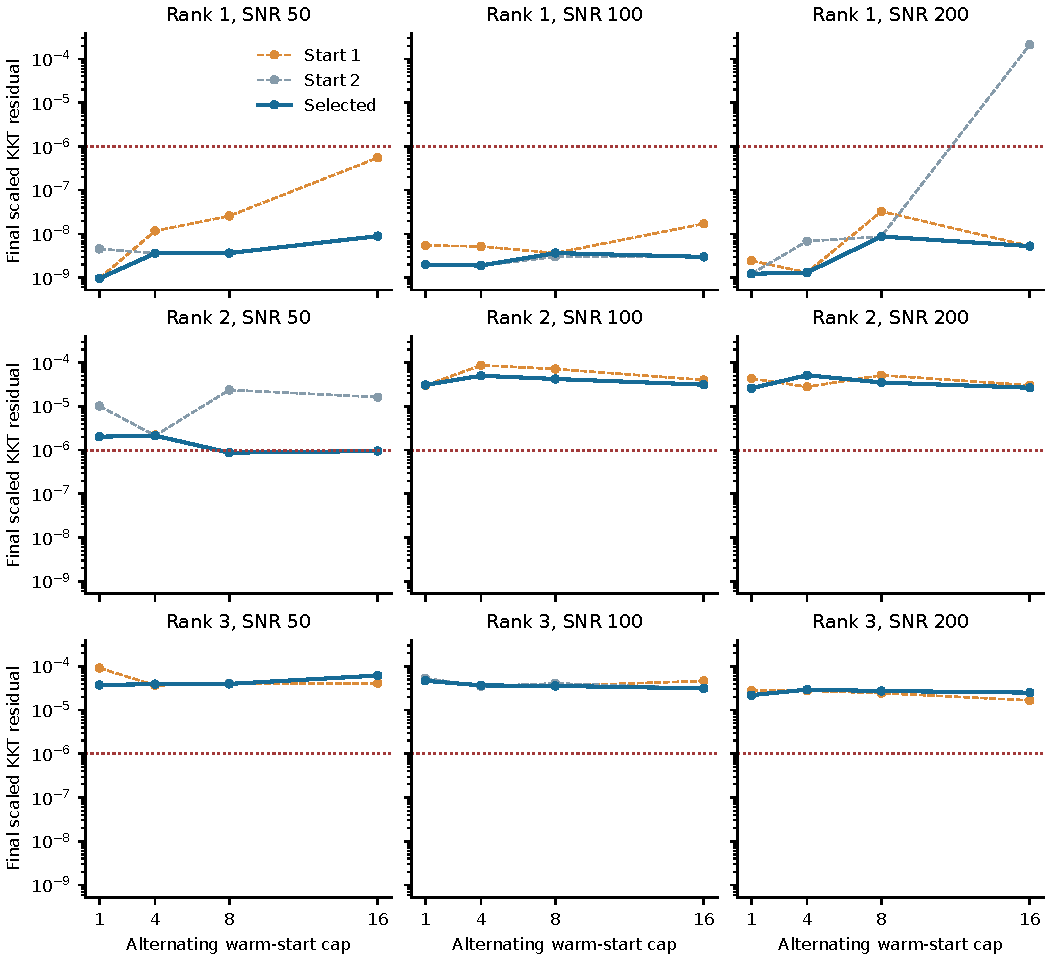
\includegraphics[width=11cm]{figures/mf_convergence_kkt.pdf}

\caption{Controlled 
 TRAIn-MF warm-start sensitivity with a common subsequent
SQP budget. Numerical stationarity is assessed by the declared independent
KKT criterion; all unresolved outcomes are retained. Repeated budgets on
one rank/SNR input are paired conditions rather than new independent samples. Orange dashed and blue-gray dashed curves denote the first and second initializations, respectively; the solid blue curve denotes the selected fit. The red dotted line marks the KKT tolerance of $10^{-6}$.}
\label{fig:mfconvergencerevision}

\end{figure}



\subsection{Factorial Separation of the Shared Selection~Stages}
\label{app:factorialcomplete}
% Draft fragment only; no manuscript sources modified.

We added a paired $2\times2$ intervention on the 36 signal-present atomic
problems, with~a common proposal bank per method constructed from 18 fitting
rows, six reserved rows and the same final 24-row refit. $S=1$ forces the
conditional spectral mask and $S=0$ retains unrestricted amplitudes.
$P=0$ retains the native-selected nominal proposal order, whereas $P=1$
applies predictive order selection. Unsupported rates may disappear during
refinement, so the nominal proposal order is not necessarily the final active
order. The~separate production reference permits both screened and unrestricted
candidates and reproduces the published selector; it is not a factorial~cell.



All 
 360 final outputs, including the separate production references, passed
their numerical checks; no selected candidate failed its numerical criterion.
The leakage interaction $(S1P1-S0P1)-(S1P0-S0P0)$ is $-1.511$ percentage
points for RAI (paired problem-bootstrap 95\% interval $[-2.603,-0.598]$)
and $-0.763$ for DOME ($[-1.670,-0.186]$). These descriptive intervals do
not establish a universal interaction or provide multiplicity-adjusted inference.
The two final proposal paths remain effectively equivalent. DOME's unmatched
mass increases slightly from $S1P0$ to $S1P1$ despite lower average leakage and
prediction error. Original signal masks are retained, including their original
internal validation reuse; this is a matched mechanism comparison, not a new
calibration experiment. Per-arm logical cost accounts for shared candidate
fits and does not represent separately measured end-to-end timing.
In the weak-component problem \texttt{test\_011\_weak}, forced screening and
prediction return three rates but match only two true rates; the minority rate
remains unrecovered. Its lower $E_U$ and $W_{1,h}$ therefore do not establish
recovery of the additional species. Correct order rises from 25 to 26 problems
relative to production choice, while complete recovery remains 23/36 for~both.

\begin{table}[H]
\caption{Matched 
 factorial experiment. Leakage and unmatched mass (UM) are
percentages. Recovery requires both order and log-rate matching.}
\label{tab:revision-factorial}

\begin{adjustwidth}{-\extralength}{0cm}
%\centering %% If there is a figure in wide page, please release command \centering


\begin{tabularx}{\fulllength}{LLRRRRR}
\toprule
\textbf{Path} & \textbf{Cell} & \textbf{Leakage} & \textbf{UM} & \boldmath{$E_U$} & \boldmath{$W_{1,h}$} & \textbf{Recovery} \\
\midrule
RAI & $S0P0$ & 6.092 & 8.627 & 0.30677 & 0.16805 & 15/36 \\
RAI & $S1P0$ & 5.301 & 8.627 & 0.29087 & 0.15092 & 15/36 \\
RAI & $S0P1$ & 3.952 & 8.016 & 0.26189 & 0.14512 & 20/36 \\
RAI & $S1P1$ & 1.650 & 7.265 & 0.23145 & 0.10767 & 23/36 \\
DOME & $S0P0$ & 3.952 & 8.016 & 0.26189 & 0.14512 & 20/36 \\
DOME & $S1P0$ & 2.413 & 7.257 & 0.23856 & 0.11588 & 21/36 \\
DOME & $S0P1$ & 3.952 & 8.016 & 0.26189 & 0.14512 & 20/36 \\
DOME & $S1P1$ & 1.650 & 7.265 & 0.23145 & 0.10767 & 23/36 \\
Both & Production & 1.728 & 7.257 & 0.23299 & 0.10944 & 23/36 \\
\bottomrule
\end{tabularx}
\end{adjustwidth}
\end{table}




\subsection{Adaptive Weak-Component~Recovery}\label{app:weakpower}
Ninety-six new problems span four generating minority-amplitude factors: 0.02, 0.04, 0.08 and 0.16. Three SNRs (50, 100 and 200), with~eight independent truth/noise realizations per cell, complete the design. Each factor multiplies the third spectral
template before the total unattenuated signal is normalized; it is not a
molar fraction. The~mask is formed from fitting acquisitions only, excluding
both internal validation and external test rows. The~frozen adaptive selector
and rate-matching tolerance remain~unchanged.


All 
 192 method fits pass their numerical criteria. RAI-S matches the minority
rate in 45 of 96 problems and DOME-S in 44 of 96; these are paired method
results, not\linebreak   192 independent chemical mixtures. At~factor 0.02 the counts
across increasing SNR are $(0,0,1)/8$ for both methods. At~factor 0.08 they
are $(1,8,8)/8$. The~intermediate factor 0.04 gives $(0,1,4)/8$ for RAI-S
and $(0,0,4)/8$ for DOME-S. These visible failures prevent a general claim
of reliable weak-component discovery. Masking also contributes: mean retained
minority spectral mass varies from about 0.59 at the weakest low-SNR cell to
0.99 at the strongest high-SNR cell. A~channel outside the mask is~unestimated.

Exact two-sided 95\% Clopper--Pearson intervals are retained per cell in the
machine-readable supplement; for example, zero of eight gives an upper
endpoint 0.369 and eight of eight a lower endpoint 0.631. They are descriptive
cell-wise intervals without multiplicity adjustment. Aggregate counts across
the prespecified SNR/factor mixture are not a universal power~guarantee.




\begin{figure}[H]

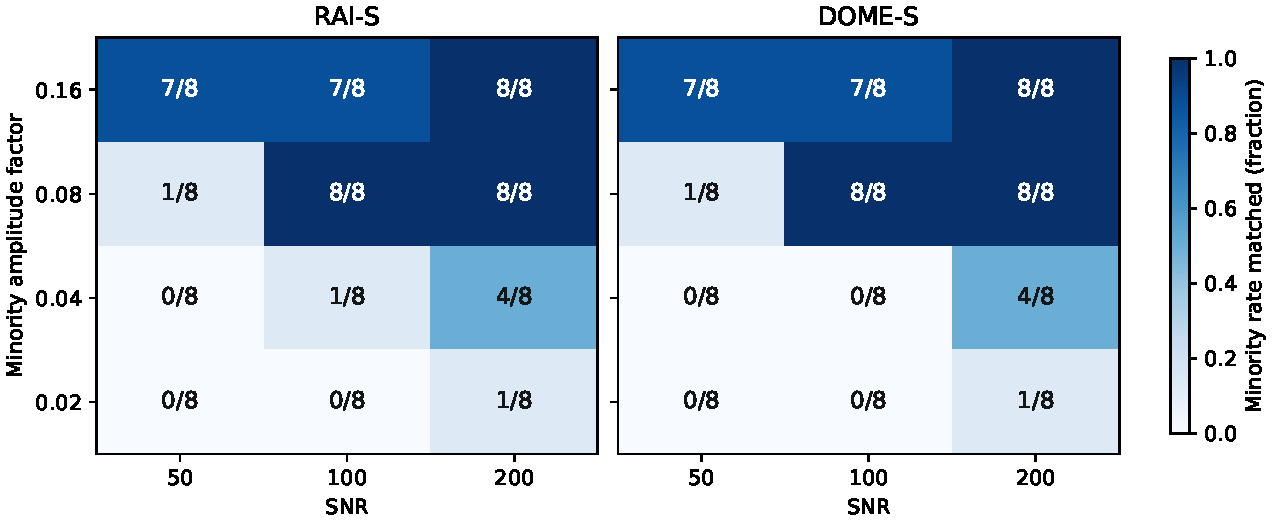
\includegraphics[width=11cm]{figures/weak_power.pdf}

\caption{\textls[-15]{New weak-component panel. Each cell counts matched minority rates in
eight independent problems, using the original log-rate tolerance 0.25.
The methods use paired inputs. These counts estimate recovery under the
declared generator, not a calibrated probability of chemical presence.}}
\label{fig:weakpowerrevision}
\end{figure}


\subsection{Expanded Neural Policy~Evaluation}

\label{app:neuralexpanded}
We trained five CPU networks with different seeds using the same 80-problem
trace bank. Each run separates 64 training from 16 validation problems and uses
training records alone to normalize features.
The new test panel contains\linebreak   120 problems: 72 in the original physical domain,
24 at unseen SNRs (25, 35 and 500), and~24 with unseen acquisition exponents
and diffusion weightings. The~five policies and the deterministic proposal-order
control share the six-round cap, a~shortlist of one with fallback, and~the same
numerical verifier. The~control is the classical shortlist variant; it differs
from both the exhaustive controller and the atomic RAI~estimator.
\begin{table}[H]
\caption{Independent 
 neural evaluation. $W_{1,h}$ averages 105 signal-present problems; $E_U$ includes all 120 problems, including 15 null controls. Numerical success is a solver criterion. Times are mean solver seconds and exclude checkpoint loading and~serialization.}
\label{tab:neuralexpanded}


\begin{adjustwidth}{-\extralength}{0cm}
%\centering %% If there is a figure in wide page, please release command \centering


\begin{tabularx}{\fulllength}{LRRRRR}
\toprule
\textbf{Method} & \boldmath{$W_{1,h}$} & \boldmath{$E_U$} & \textbf{Numerical Success} & \textbf{Seconds} & \textbf{Tree Fits} \\
\midrule
Classical shortlist & 0.33383 & 0.29961 & 120/120 & 22.03 & 20.76 \\
RAI-Net 172901 & 0.33341 & 0.29956 & 120/120 & 17.44 & 19.24 \\
RAI-Net 172902 & 0.33319 & 0.29941 & 120/120 & 18.91 & 19.66 \\
RAI-Net 172903 & 0.33323 & 0.29952 & 120/120 & 18.13 & 19.49 \\
RAI-Net 172904 & 0.33390 & 0.29951 & 120/120 & 18.87 & 18.94 \\
RAI-Net 172905 & 0.33271 & 0.29944 & 120/120 & 19.15 & 19.55 \\
\bottomrule
\end{tabularx}
\end{adjustwidth}
\end{table}

The seed-average neural-minus-classical $W_{1,h}$ difference is $-0.00054$ (paired problem-bootstrap 95\% interval $[-0.00174, 0.00056]$); the corresponding $E_U$ difference is $-0.00012$ ($[-0.00044, 0.00010]$). The~pooled bootstrap resamples whole problems within each domain, preserving domain counts; the five seed outputs on a problem are paired, not independent tests. Individual seed mean $W_{1,h}$ differences range from $-0.00111$ to $0.00007$.
ID: $\Delta W_1=-0.00136$, interval $[-0.00294, -0.00003]$ ($n=63$); individual seed differences range from $-0.00165$ to $-0.00076$. OOD\_noise: $\Delta W_1=-0.00059$, interval $[-0.00230, 0.00070]$ ($n=21$); individual seed differences range from $-0.00142$ to $0.00013$. OOD\_acquisition: $\Delta W_1=0.00197$, interval $[-0.00135, 0.00559]$ ($n=21$); individual seed differences range from $-0.00106$ to $0.00430$.
All 720 final method outputs pass their numerical checks, with\linebreak  0 execution errors
and 0 failed final checks. The~analysis retains failed numerical outputs whenever
they occur, rather than removing them from the averages.
Intermediate failures still occur: 98/2371 control subproblems and 476/11026 neural
subproblems fail the search-stage checks, with~91--99 failures per policy. Each
method encounters at least one failed search fit in 48/120 problems. The~selected
training paths and all final refits nevertheless pass their checks. These counts
describe solver events and should not be treated as independent statistical trials.
Mean differences from the classical control are $-3.524$ s per problem
for solver time and $-1.382$ for the number of fixed-tree fits (neural minus
classical). Equal search caps therefore do not imply equal realized effort.
Training the five policies took 3.455 s after data loading. Generating the common training traces took 1690.7 s of summed computation; that sum cannot be compared directly with wall-clock time.
These measurements do not establish an end-to-end speedup. Four selected
checkpoints reach the 400-epoch budget, so learning convergence is also unresolved.
The study supports neither a universal accuracy advantage nor experimental
chemical~identification.

An exploratory breakdown by problem family finds lower mean shape error for
all five policies on the 15 broad-profile problems, but~higher error for four
of the five policies on the 90 atomic problems. We did not use these patterns
to select a seed or tune the models. They are post hoc observations, not
independent confirmatory~tests.

\begin{figure}[H]

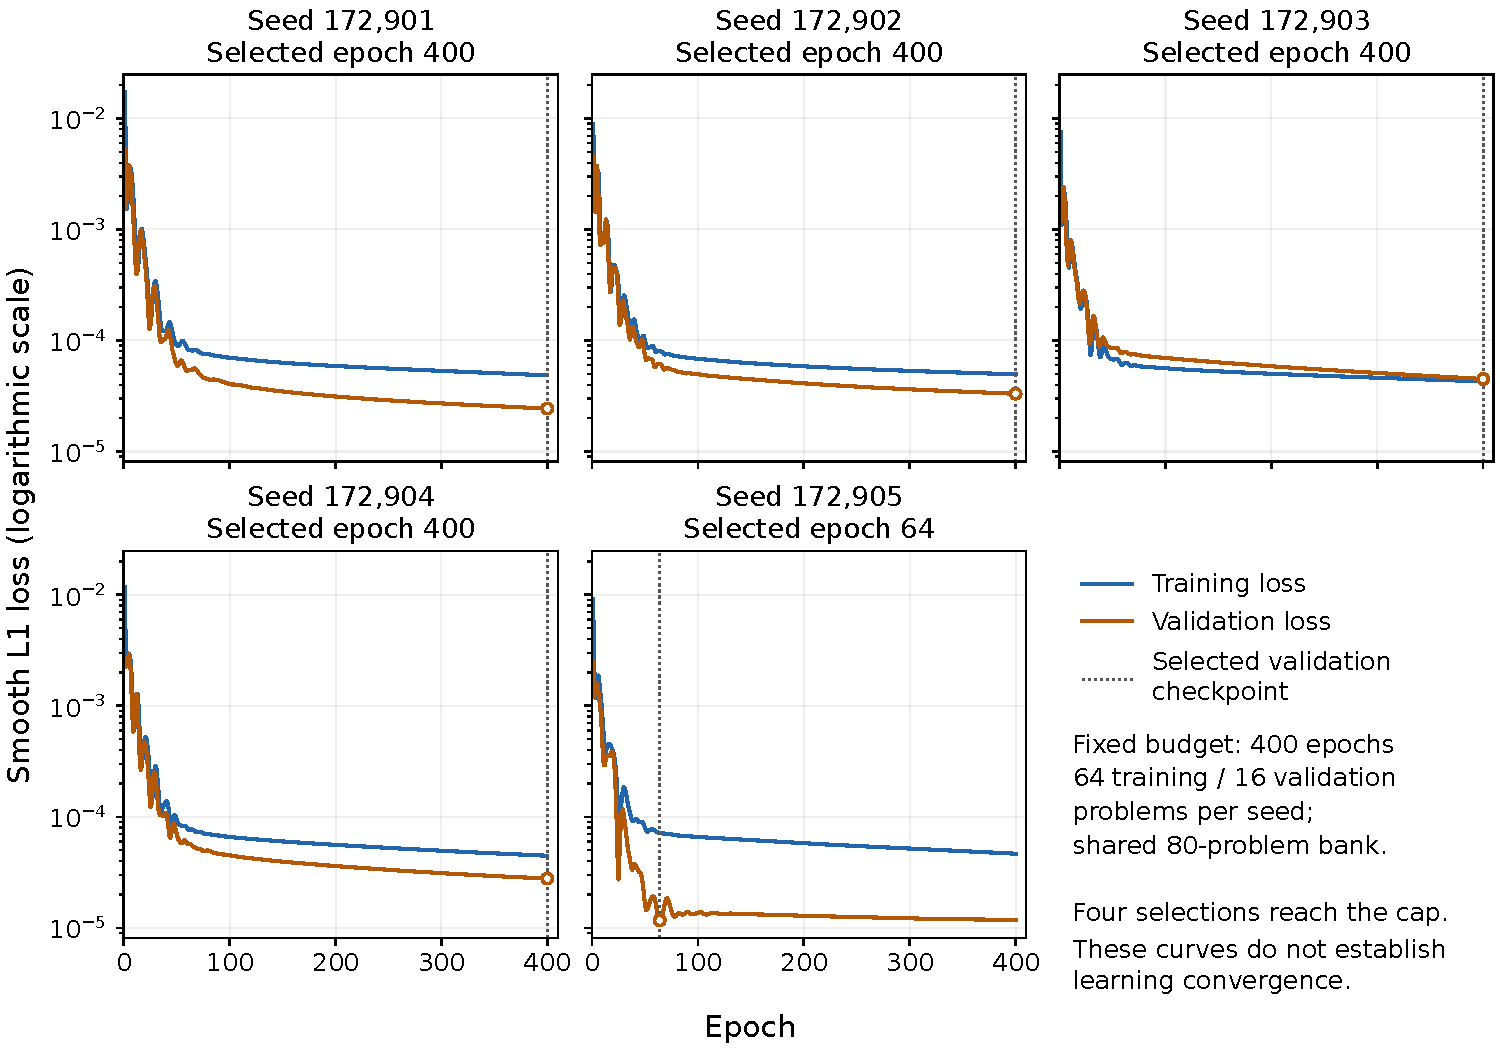
\includegraphics[width=13cm]{figures/neural_learning_curves.pdf}

\caption{Training 
 and whole-problem validation Smooth L1 loss for five separately
seeded RAI-Net rankers. Each run uses 64 training and 16 validation problems
from the same historical 80-problem bank. Dotted lines and open markers
identify the lowest observed validation loss checkpoint. Four selections
reach the declared 400-epoch budget, so these histories do not establish
learning convergence. The~historical trainer records training loss before
the Adam update and validation loss after it. Test observations are absent from normalization,
training and checkpoint selection.}\label{fig:neurallearning}

\end{figure}



\subsection{Shared External-Reference~Comparison}\label{app:externalcomparison}
The additional comparison uses the same frozen observations, masks and outer
test acquisitions. The~physical interval is common to grid methods and
positive measure eligibility. Native continuous fits are retained with their
original rate constraints rather than silently projected into that interval. Matrix
zero served as an adapter pilot and is retained in the raw outputs but excluded
symmetrically from the iid summary, leaving 47 matrices (41 signal-present and
six null). Twelve underlying signal-present problems also receive each of the
baseline and correlated-noise stresses. These are retrospective comparisons,
not a new untouched synthetic population. Outer test rows are not used in
the internal parameter or order~decisions.

SCORE uses the attributed GNAT translation, signed conditional least squares
and its original initialization, with~a declared reserved-acquisition wrapper
selecting orders zero through four. Candidate selection enforces interval
eligibility, but~the final continuous refit is unconstrained in log rate;
out-of-interval results are retained and flagged. The~positive-amplitude
sensitivity uses the same wrapper and proposal budget. LOCODOSY retains its native local SVD
order and reduction rules on the common contiguous signal windows; its sum of
local components is not a global molecular count. Its native rate domain has
zero as the lower limit and the common upper limit. LOCODOSY uses the training
observations for its order rule; only the validation-selected adapters use
the internal split. Five of the 47 iid LOCODOSY outputs contain rates outside
the declared positive measure interval; none is projected or discarded.
No outer test row participates in these decisions. Positive Tikhonov selects
its curvature weight from $\{0.01,1,100,10^4\}$ on internal validation.
The PALMA constrained objective uses a training-only positive low-$b$ scale,
entropy weights $\{0.01,0.1,0.5\}$ selected on internal validation, a~declared
95\% Gaussian noise-ball radius and 5000 final PPXA+ iterations. A~batched
Woodbury graph projection was checked against the reviewed scalar QR engine;
this is an implementation of the stated objective, not a claim of identical
performance to all upstream application~presets.

\begin{table}[H]\small
\caption{Common 
 external-reference comparison. $E_U$ is clean external error
in noise units over signal-present cases. Numerical success uses each method's
own criterion; all returned outputs enter $E_U$, including nonconverged ones.
The column $n$ counts only outputs admitting a nonnegative
measure within the declared interval and is therefore a different population
for signed methods.}\label{tab:externalexecuted}
\begin{tabularx}{\textwidth}{LRRRR}\toprule
\textbf{Method} & \textbf{Numerical Success} & \boldmath{$E_U$} & \boldmath{$W_{1,h}$} & \textbf{n}\\\midrule
RAI-S & 47/47 & 0.23477 & 0.1201 & 41 
\\
DOME-S & 47/47 & 0.23477 & 0.1201 & 41\\
SCORE-CV (signed) & 47/47 & 0.30329 & 0.0000 & 3\\
SCORE-NNLS-CV & 47/47 & 0.26681 & 0.1563 & 41\\
LOCODOSY (signed) & 47/47 & 0.26114 & 0.0013 & 4\\
Positive Tikhonov & 47/47 & 0.33523 & 0.3057 & 41\\
PALMA objective + CV & 0/47 & 0.73627 & 0.4225 & 41\\
\bottomrule\end{tabularx}\end{table}

The table compares prediction under the stated fitting conditions, rather than
chemical identification. Signed cancellation can reduce error without yielding
a positive component representation. Similarly, PPXA+ has not reached the required
optimality criterion for the PALMA objective, so its finite-budget result cannot
rank the fully optimized method. The~supplement retains all convergence flags
and curve-level constraint diagnostics. CONTIN, UPEN, DRECT and DREAM were not
run under this common protocol; Table~\ref{tab:externalmethods} states what those
comparisons would require. Positive Tikhonov is a separate control and is not
presented as the full CONTIN procedure. The~executed comparisons cover the
closest joint-component references and two positive distributional~controls.

On the twelve baseline-stress cases, positive SCORE has a slightly smaller
mean clean error than RAI-S ($1.00044$ versus $1.01092$ noise units); the
paired descriptive interval for the difference is $[-0.02583,0.00196]$ and
includes zero. There is no demonstrated robust advantage on this offset
panel. Correlated-noise results and all paired contrasts are included in
the machine-readable supplement; they are not independent replications of
the underlying twelve signal~configurations.


\subsection{Experimental Prediction on Industrial Resin~Spectra}\label{app:experimentalrevision}
We analysed spectra from four industrial resin specimens identified as TP194-2623086, TP194-2623088, TP194-2623084 and TP194-2619082. These are specimen identifiers; their digits are retained without thousands separators. 
 Each series contains three blocks at diffusion times 75, 100
and 125~ms, with~23 acquisitions and 65,536 spectral channels per block. The~twelve
blocks belong to four specimens and are not independent mixture preparations.
We fit all \mbox{17,386--21,314 channels} per block within the detected positive absorption
support, preserving their measured signs. Five acquisitions are withheld for
prediction, and~support detection also excludes the internal validation rows.
A single scalar normalizes each matrix; channels are neither rescaled individually
nor replaced by integrated bands or a thinned fit grid. Outside the support,
signal remains unestimated. The~full-spectrum check detects 75--219 strongly
negative points per block, including 53--187 outside the positive support.
We apply no automatic phase, baseline, absolute-value or clipping~correction.

RAI-S and DOME-S use their frozen support-aware estimators with a four-atom search cap. SCORE-CV uses the attributed SCORE implementation with signed amplitudes and native initialization, augmented by internal acquisition-based order selection over one to four atoms~\cite{score}. SCORE-NNLS-CV changes the conditional amplitude problem to NNLS while retaining the same initialization, optimizer budget and selection wrapper; it is explicitly a constrained variant, not the original signed SCORE method. LOCODOSY-SCORE retains the native local singular-value order heuristic and reduction rules~\cite{locodosy}, using the same detected windows. Its output rows are local contributions, not a global species count. Small-rank batched NNLS is checked against the native per-channel solver; the RAI objective, gradient and predictions are also checked against the original implementation. All selected channels contribute to every reported~error.

\begin{table}[H]
\caption{Experimental 
 acquisition holdout prediction on twelve blocks, grouped into four industrial resin specimens. NRMSE divides held-out RMSE by the training RMS on the same support. NC counts final global optimizer nonconvergence; unstable flags denote kernel condition above $10^8$ or amplitude expansion above $10^4$; cap counts selection of the maximum four global atoms. These flags are not exclusions. Dashes denote quantities that are not global estimands for~LOCODOSY.}\label{tab:experimentalrevision}
\centering\small
\begin{tabularx}{\textwidth}{LRRRRR}\toprule
\textbf{Method} & \textbf{Mean NRMSE (\%)} & \textbf{Median (\%) }& \textbf{NC} & \textbf{Unstable} & \textbf{Cap}\\\midrule
RAI-S & 1.1226 & 1.1119 & 0 & 0 & 12\\
DOME-S & 1.1226 & 1.1119 & 0 & 0 & 12\\
SCORE-CV & 0.7740 & 0.7884 & 6 & 8 & 8\\
SCORE-NNLS-CV & 1.1230 & 1.1119 & 0 & 0 & 12\\
LOCODOSY-SCORE & 0.8914 & 0.8620 & -- & -- & --\\
\bottomrule\end{tabularx}
\end{table}

All 60 of 60 planned predictions were completed. RAI-S and DOME-S reach the cap
and trigger the atomic model mismatch warning in all twelve blocks. Their largest
relative prediction difference is $1.41\times10^{-12}$, providing no independent
predictive advantage for either proposal mechanism. Reaching the cap also does
not establish four chemical species. Positive SCORE serves as a constraint
control. Signed SCORE predicts better in several blocks, but~6 of its twelve
final fits fail to converge within the budget and 8 have unstable global
amplitudes. We retain these predictions in the table. LOCODOSY covers\linebreak   174 windows,
with 0 nonconverged local fits and 0 failed windows. Low prediction error from
canceling signed amplitudes alone cannot establish reliable~identification.


Background neighboring-channel correlations range from 0.999198 to 0.999757. Consequently, the~background MAD scale is descriptive, and~these processed data do not validate an independent-Gaussian interpretation of support scores or channel-wise confidence intervals. Acquisition-order effects and residual phase/baseline distortion are not separately identified. Spectral-factor matching across the three diffusion times is reported as a descriptive consistency check, not as chemically verified~correspondence.

The same HDO-based calibration was used at all three diffusion times. If~$D=10^{-9}c\kappa$, where $c$ is the calibration coefficient, first-order uncertainty propagation would require
\begin{equation}
 \operatorname{Var}(D)\simeq 10^{-18}\left[\kappa^2\operatorname{Var}(c)+c^2\operatorname{Var}(\kappa)+2c\kappa\operatorname{Cov}(c,\kappa)\right].
\end{equation}

The reference and thermal-model contributions to $\operatorname{Var}(c)$ are not quantified in the source calibration; they are not set to zero. The~maps are conditional on that calibration, and~no absolute diffusion-accuracy interval or molecular-weight estimate is~asserted.

The available records do not link these four identifiers to a verified composition.
We therefore assign no compositions or diffusion values from other batches to
these specimens. The~measurements provide evidence about prediction on industrial
resins, but~not a test against known component counts or independently measured
component diffusion coefficients. This is especially relevant when finite atomic
models are fitted to potentially polydisperse~materials.

\begin{figure}[H]

\begin{adjustwidth}{-\extralength}{0cm}
\centering %% If there is a figure in wide page, please release command \centering


\centering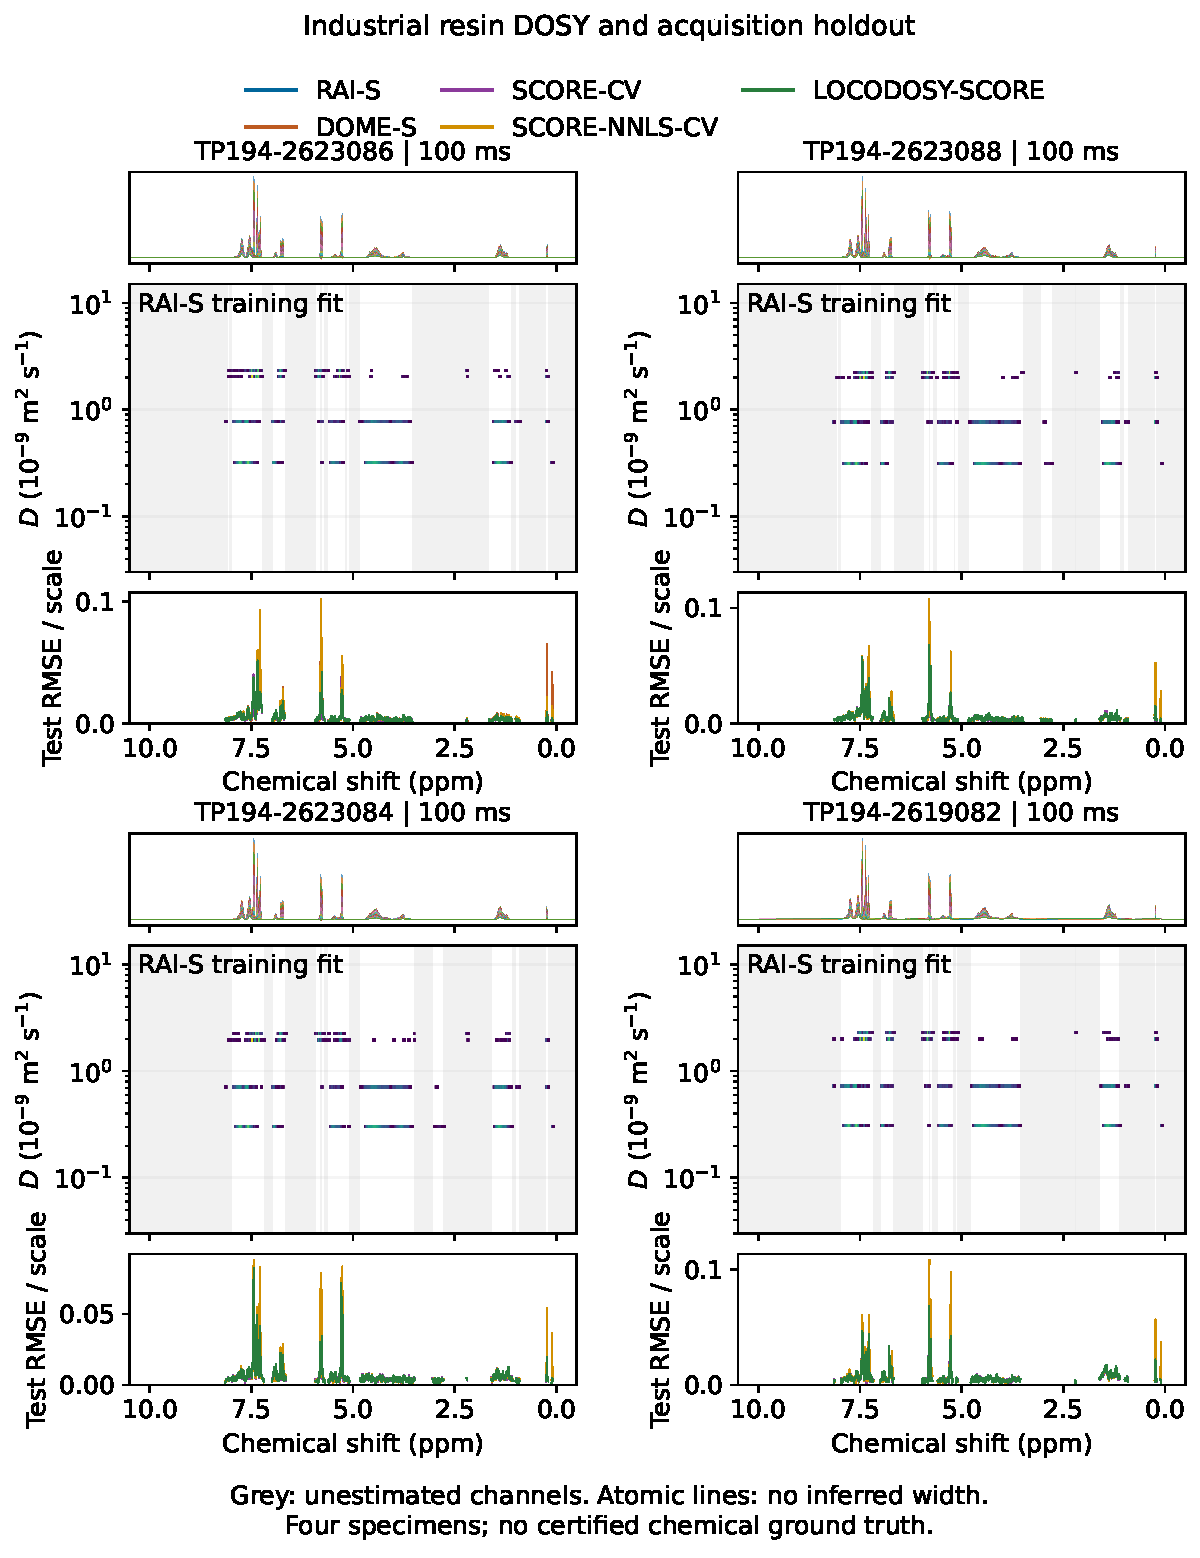
\includegraphics[width=16.5cm]{figures/experimental_four_series.pdf}
\end{adjustwidth}
\caption{Industrial 
 resin spectra at 100~ms: measured spectral families (top), RAI-S training-fit atomic DOSY maps (middle) and held-out error profiles for the five estimators (bottom). All detected support channels enter the fits; gray map regions are unestimated. Display thinning is confined to traces and error curves. Atoms are shown without fabricated distributional widths, and~no chemical ground-truth map is~available. The TP194 labels are specimen identifiers, not measured quantities.}\label{fig:experimentalresins}

\end{figure}

\begin{figure}[H]
\begin{adjustwidth}{-\extralength}{0cm}
\centering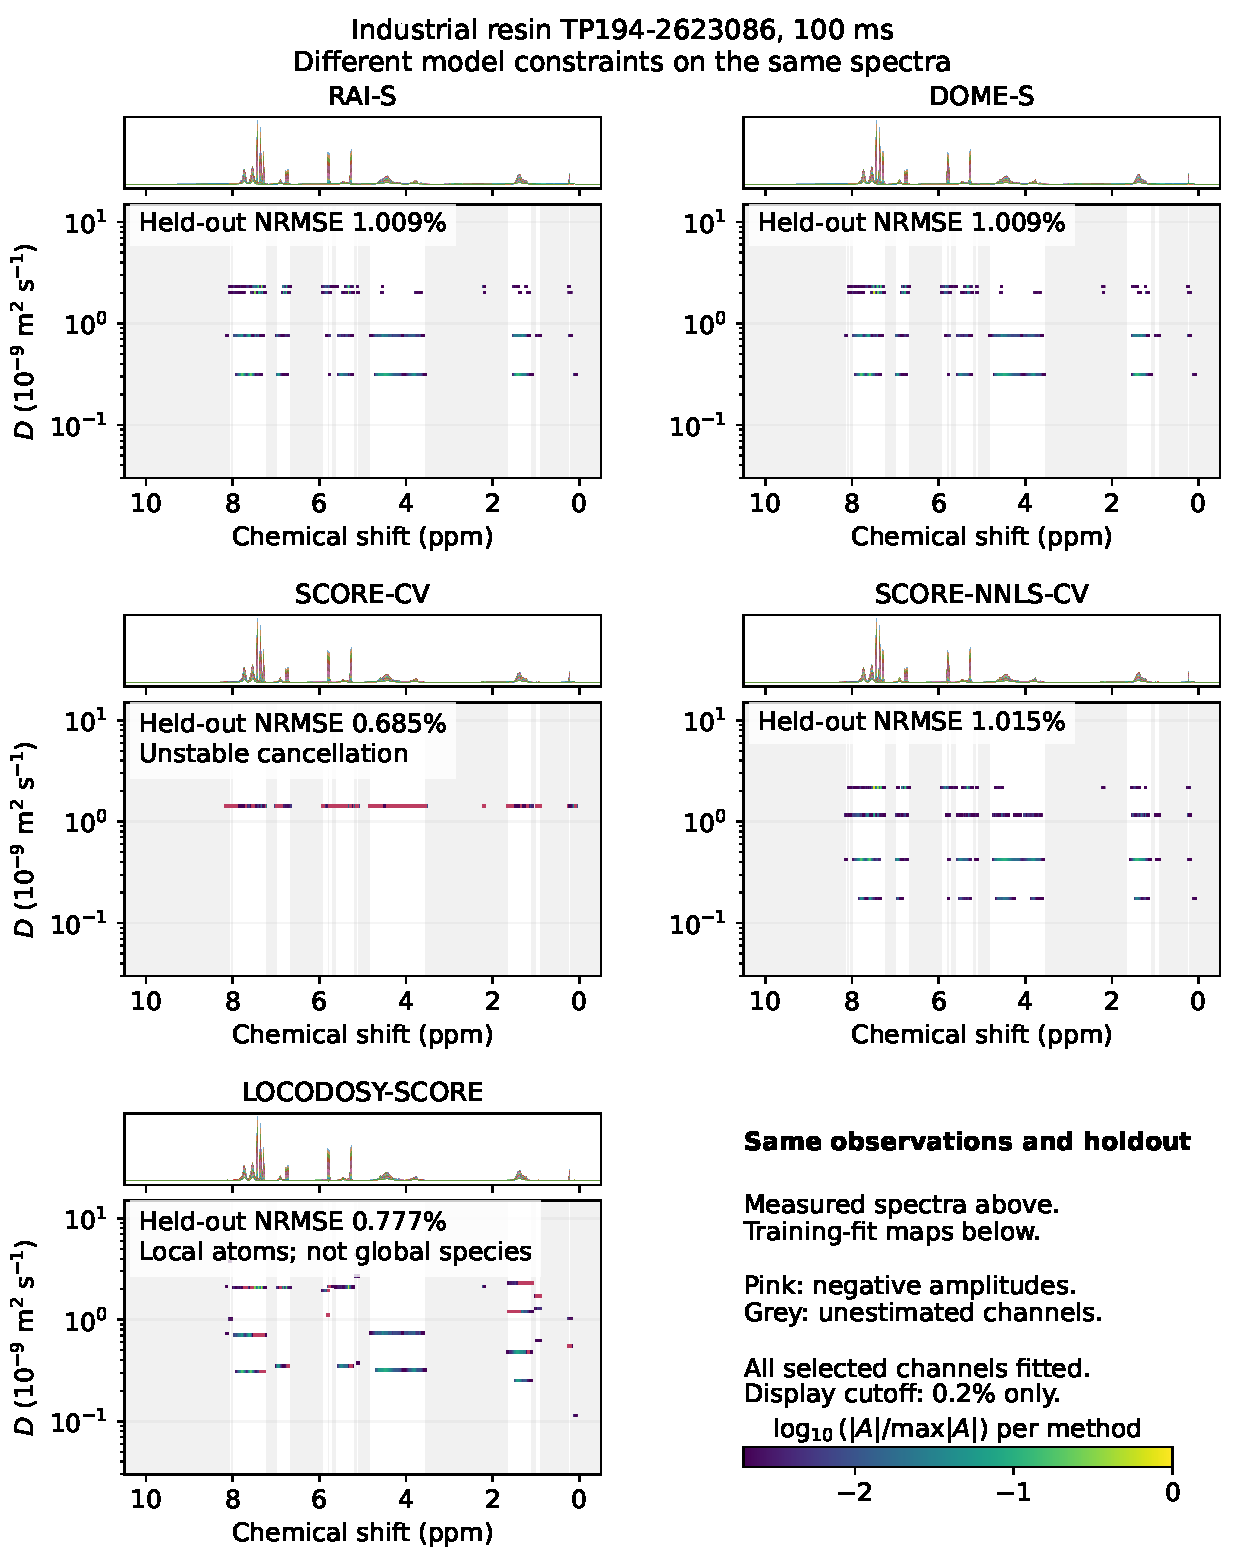
\includegraphics[width=16.5cm]{figures/experimental_methods_T1_B2.pdf}
\end{adjustwidth}
\caption{The 
 five estimators on industrial resin TP194-2623086 at 100~ms, using identical observations and acquisition holdout. Colors show relative absolute amplitude within each method; negative amplitudes are pink and unestimated regions are gray. The~0.2\% display cutoff does not affect fitting or scoring. The~nearly coincident signed SCORE atoms exhibit large cancellation despite a lower held-out prediction error. LOCODOSY lines are local~contributions. TP194-2623086 is a specimen identifier and is therefore written without thousands separators.}\label{fig:experimentalmethods}

\end{figure}



\subsection{A Public Multicomponent DOSY~Example}\label{app:publicmixture}
We additionally processed the public \texttt{PropPentSuc\_DOSY.fid} example
distributed by the official DOSY Toolbox downloads page~\cite{dosytoolboxdata}.
Its internal sample text documents propanol and sucrose in D$_2$O; its directory
name is consistent with the 1-propanol/1-pentanol/sucrose example illustrated
in the GNAT manual~\cite{gnatmanual}. The~latter does not explicitly identify
this archived file, so pentanol is not treated as a verified additional label.
Neither a certified complete composition nor independently measured diffusion
coefficients accompany the example used here. It therefore supplies a public
multicomponent experimental check, not known-order or absolute-$D$ ground~truth.

The archive contains 30 acquired gradient levels. Acquisitions
4, 8, 12, 16, 20, 24 and 28 were reserved for external prediction;
five of the remaining acquisitions formed the internal validation split.
A single common linear ACME phase~\cite{acme} was estimated from the other
18 discovery acquisitions after Fourier transformation and then frozen for
all methods and acquisitions. The~archived phase alone had left visible
dispersion in discovery-only quality control. We applied no baseline
subtraction, absolute-value rectification or spectral alignment.
All 4074 original spectral channels within the discovery-detected positive
absorption support were retained from the 32,768-point spectrum. Channels
outside that support remain unestimated. The~common order cap was~four.

Following the GNAT Varian import convention, the~nominal encoding was
\begin{equation}
b_i=\gamma^2 T_{\mathrm{enc}}
 \bigl(g_{i,\mathrm{DAC}}c_{\mathrm{DAC}}\,10^{-2}\bigr)^2,
\end{equation}
where $T_{\mathrm{enc}}$ is the archived \texttt{dosytimecubed} parameter and
$c_{\mathrm{DAC}}$ is the archived conversion to G\,cm$^{-1}$.
The same homogeneous gradient kernel was used for every method.
No independent gradient calibration could be matched to this acquisition, so no further gradient correction was applied.
Nonuniform gradients and other unmodeled acquisition effects therefore
remain possible explanations for residual curvature; the nominal $D$ scale
is not an independently calibrated accuracy~claim.

\begin{table}[H]
\caption{One 
 public experimental dataset, shared support and acquisition
holdout. Numerical convergence and chemical identification are distinct.}
\label{tab:publicmixturerevision}
\small
\begin{tabularx}{\textwidth}{LRRL}\toprule
\textbf{Method} & \textbf{Test NRMSE} \textbf{(\%)} & \textbf{Atoms} & \textbf{Converged} \\ \midrule
RAI-S & 0.582 & 4 & yes \\
DOME-S & 0.582 & 4 & yes \\
SCORE-CV & 0.232 & 4 & yes \\
SCORE-NNLS-CV & 0.582 & 4 & yes \\
LOCODOSY-SCORE & 0.270 & 31 $^{*}$ & local \\
\bottomrule\end{tabularx}


\noindent{\small{$^{*}$ Sum of local contributions, not a global
molecular count. All local solver calls converged.}}
%\par\smallskip\footnotesize $^{*}$Sum of local contributions, not a global
%molecular count. All local solver calls converged.
\end{table}

RAI-S and DOME-S returned effectively identical predictions (relative
difference $7.6\times10^{-11}$), both reaching the cap and activating the
atomic model mismatch diagnostic. The~positive-amplitude SCORE variant
agreed closely with them. Signed SCORE had the lowest prediction error;
its negative-amplitude fraction was 9.54\% of total absolute amplitude.
Unlike the unstable signed fits in some resin blocks, this fit converged
and was not flagged by the declared kernel conditioning or amplitude expansion
checks. Thus, its predictive advantage cannot be dismissed as numerical failure,
although a signed decomposition does not establish nonnegative constituent
spectra. LOCODOSY also predicted better than the positive global fits.
These results do not demonstrate superiority of RAI-S or DOME-S over the
references, or~an independent benefit of their proposal mechanisms.
The single archived experiment, correlated processed noise
(adjacent background correlation 0.983), unknown full composition and nominal
gradient calibration preclude a population-level detection claim or certified
chemical assignments. Solvent/reference resonances were not silently removed,
and an atomic row is not equated with a~molecule.

\begin{figure}[H]
\begin{adjustwidth}{-\extralength}{0cm}
\centering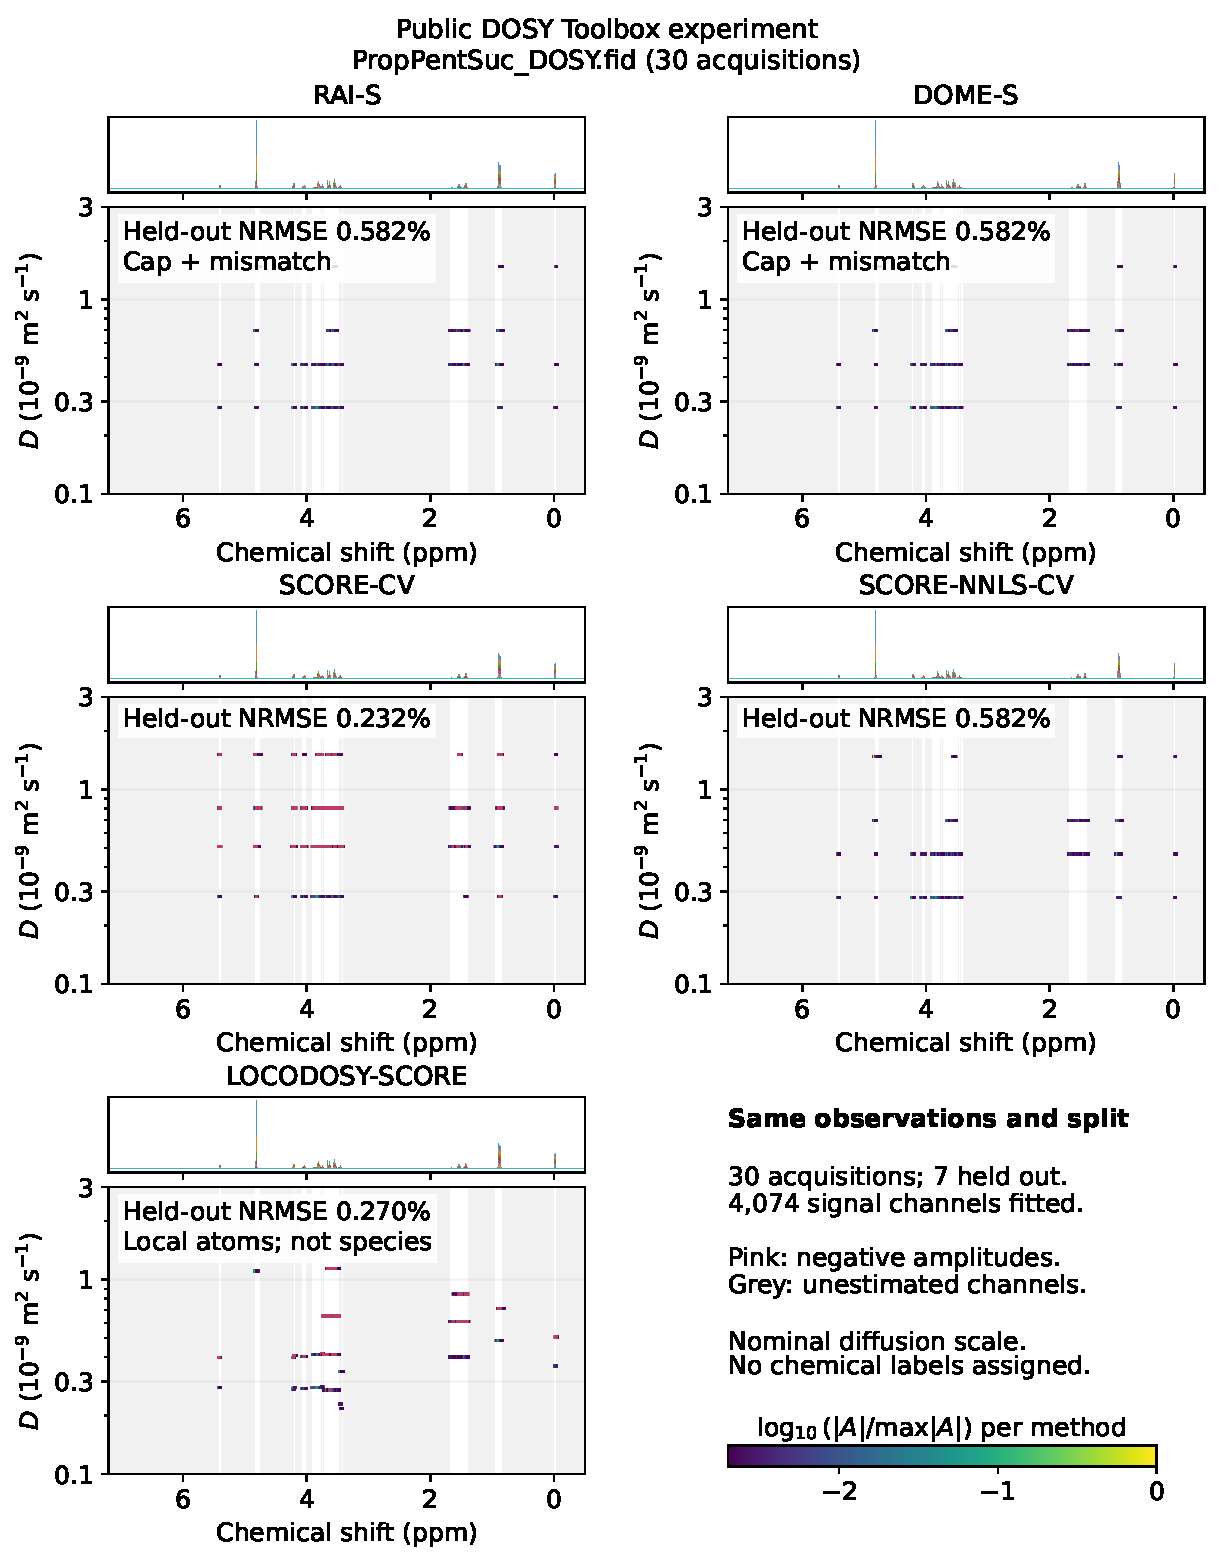
\includegraphics[width=15.8cm]{figures/public_mixture_comparison.pdf}
\end{adjustwidth}
\caption{Public DOSY Toolbox example. Measured spectral families appear above
the training-only fitted atomic maps. Every selected spectral channel is fitted;
only the display of the upper traces is decimated. Pink denotes signed negative
amplitudes, gray denotes unestimated channels, and~the 0.2\% relative display
cutoff does not prune the fit. Atomic rows have no inferred diffusion width or
assigned chemical identity.}
\label{fig:publicmixturerevision}

\end{figure}





\reftitle{References}

\begin{adjustwidth}{-\extralength}{0cm}
%\centering %% If there is a figure in wide page, please release command \centering


\begin{thebibliography}{99}
%\input{references}

\bibitem{stejskal}
Stejskal, E.O.; Tanner, J.E. Spin Diffusion Measurements: Spin Echoes in the Presence of a Time-Dependent Field Gradient. \emph{J. Chem. Phys.} \textbf{1965}, \emph{42}, 288--292. \url{https://doi.org/10.1063/1.1695690}.

\bibitem{morris}
Morris, K.F.; Johnson, C.S., Jr. Diffusion-ordered two-dimensional nuclear magnetic resonance spectroscopy. \emph{J. Am. Chem. Soc.} \textbf{1992}, \emph{114}, 3139--3141. \url{https://doi.org/10.1021/ja00034a071}.

\bibitem{contin}
Provencher, S.W. CONTIN: A general purpose constrained regularization program for inverting noisy linear algebraic and integral equations. \emph{Comput. Phys. Commun.} \textbf{1982}, \emph{27}, 229--242. \url{https://doi.org/10.1016/0010-4655(82)90174-6}.

\bibitem{train}
Xu, K.; Zhang, S. Trust-Region Algorithm for the Inversion of Molecular Diffusion NMR Data. \emph{Anal. Chem.} \textbf{2014}, \emph{86}, 592--599. \url{https://doi.org/10.1021/ac402698h}.

\bibitem{itamed}
Urba\'nczyk, M.; Bernin, D.; Ko\'zmi\'nski, W.; Kazimierczuk, K. Iterative Thresholding Algorithm for Multiexponential Decay Applied to PGSE NMR Data. \emph{Anal. Chem.} \textbf{2013}, \emph{85}, 1828--1833. \url{https://doi.org/10.1021/ac3032004}.

\bibitem{palma}
Cherni, A.; Chouzenoux, E.; Delsuc, M.-A. PALMA, an improved algorithm for DOSY signal processing. \emph{Analyst} \textbf{2017}, \emph{142}, 772--779. \url{https://doi.org/10.1039/C6AN01902A}.

\bibitem{kaczmarz}
Gonz\'alez-L\'azaro, M.; Viciana, E.; Valdivieso, V.; Fern\'andez, I.; Arrabal-Campos, F.M. Regularized Kaczmarz Solvers for Robust Inverse Laplace Transforms. \emph{Mathematics} \textbf{2025}, \emph{13}, 2166. \url{https://doi.org/10.3390/math13132166}.

\bibitem{silt}
Yuan, B.; Ding, Y.; Kamal, G.M.; Shao, L.; Zhou, Z.; Jiang, B.; Sun, P.; Zhang, X.; Liu, M. Reconstructing diffusion ordered NMR spectroscopy by simultaneous inversion of Laplace transform. \emph{J. Magn. Reson.} \textbf{2017}, \emph{278}, 1--7. \url{https://doi.org/10.1016/j.jmr.2017.03.004}.

\bibitem{lin}
Lin, E.; Yang, Y.; Huang, Y.; Chen, Z. High-Resolution Reconstruction for Diffusion-Ordered NMR Spectroscopy. \emph{Anal. Chem.} \textbf{2020}, \emph{92}, 634--639. \url{https://doi.org/10.1021/acs.analchem.9b03865}.

\bibitem{arrabal2016}
Arrabal-Campos, F.M.; 
 Oña-Burgos, P.; Fernández, I. Molecular weight prediction with no dependence on solvent viscosity. A quantitative pulse field gradient diffusion NMR approach. \emph{Polym. Chem.} \textbf{2016}, \emph{7}, 4326--4329. \url{https://doi.org/10.1039/c6py00691d}. Correction: \emph{Polym. Chem.} \textbf{2016}, \emph{7}, 5331; DOI: 10.1039/c6py90124g.


\bibitem{protein}
Arrabal-Campos, F.M.; Aguilera-Sáez, L.M.; Fernández, I. A diffusion NMR method for the prediction of the weight-average molecular weight of globular proteins in aqueous media of different viscosities. \emph{Anal. Methods} \textbf{2019}, \emph{11}, 142--147. \url{https://doi.org/10.1039/c8ay01817k}.

\bibitem{concentration}
Arrabal-Campos, F.M.; González-Lázaro, M.; Pérez, J.M.; Martínez Lao, J.A.; Fernández, I. Concentration-independent molecular weight determination of polymers via diffusion NMR: A universal approach across solvents. \emph{Eur. Polym. J.} \textbf{2025}, \emph{226}, 113710. \url{https://doi.org/10.1016/j.eurpolymj.2024.113710}.

\bibitem{photo2026}
Czarnota, M.; Cybularczyk-Cecotka, M.; Westermair, F.F.; Arrabal Campos, F.; Kapil, K.; Matyjaszewski, K.; Szczepaniak, G.; Urbańczyk, M. Real-time monitoring of photoinduced atom transfer radical polymerization by time-resolved diffusion NMR. \emph{Polym. Chem.} \textbf{2026}, \emph{17}, 1109--1115. \url{https://doi.org/10.1039/d6py00103c}.

\bibitem{cyclic2021}
Ruiz Martínez, C.; Pérez, J.M.; Arrabal-Campos, F.M.; Batuecas, M.; Ortuño, M.A.; Fernández, I. Cyclic polylactide synthesis initiated by a lithium anthraquinoid: Understanding the selectivity through DFT and diffusion NMR. \emph{Polym. Chem.} \textbf{2021}, \emph{12}, 4083--4092. \url{https://doi.org/10.1039/d1py00547b}.

\bibitem{cyclic2023}
Ruiz Martínez, C.; Pérez, J.M.; Arrabal-Campos, F.M.; Rodríguez-Diéguez, A.; Choquesillo-Lazarte, D.; Martínez-Lao, J.A.; Ortuño, M.A.; Fernández, I. Lithium anthraquinoids as catalysts in the ROP of lactide and caprolactone into cyclic polymers. \emph{Polym. Chem.} \textbf{2023}, \emph{14}, 452--461. \url{https://doi.org/10.1039/d2py01076c}.

\bibitem{chitosan2026}
Li, L.; Muguruza, A.R.; Arrabal-Campos, F.M.; Férnandez, T.; Fernández-García, S.; Muñoz-Flores, N.; Lorenzo, J.; Fernández, I.; Contreras-Caceres, R.; Guardia, P. Electrospun PVA-chitosan nanofibers with antibacterial properties for wound healing: Unveiling the potential of low molecular weight chitosan. \emph{J. Mater. Chem. B} \textbf{2026}, \emph{14}, 9312--9326. \url{https://doi.org/10.1039/d6tb00497k}.

\bibitem{diffga}
Arrabal-Campos, F.M.; Álvarez, J.D.; García-Sancho, A.; Fernández, I. Molecular weight prediction in polystyrene blends. Unprecedented use of a genetic algorithm in pulse field gradient spin echo (PGSE) NMR. \emph{Soft Matter} \textbf{2017}, \emph{13}, 6620--6626. \url{https://doi.org/10.1039/c7sm01569k}.

\bibitem{dart}
Arrabal-Campos, F.M.; Aguilera-Sáez, L.M.; Fernández, I. Algebraic Reconstruction Technique for Diffusion NMR Experiments. Application to the Molecular Weight Prediction of Polymers. \emph{ J. Phys. Chem. A} \textbf{2019}, \emph{123}, 943--950. \url{https://doi.org/10.1021/acs.jpca.8b08584}.

\bibitem{mfv31}
Arrabal-Campos, F.M. TRAIn-MF: MATLAB implementation for multifrequency DOSY inversion. Research software, 2026. Available online: \url{https://github.com/fmarrabal/train-dosy/blob/v0.1.0/matlab/legacy/TRAIn_DOSY_MFV31.m} (accessed on 9 November 2026).

\bibitem{golub}
Golub, G.H.; Pereyra, V. The Differentiation of Pseudo-Inverses and Nonlinear Least Squares Problems Whose Variables Separate. \emph{SIAM J. Numer. Anal.} \textbf{1973}, \emph{10}, 413--432. \url{https://doi.org/10.1137/0710036}.

\bibitem{shearer}
Shearer, P.; Gilbert, A.C. A generalization of variable elimination for separable inverse problems beyond least squares. \emph{Inverse Probl.} \textbf{2013}, \emph{29}, 045003. \url{https://doi.org/10.1088/0266-5611/29/4/045003}.

\bibitem{lawson}
Lawson, C.L.; Hanson, R.J. \emph{Solving Least Squares Problems}; Classics in Applied Mathematics; SIAM: Philadelphia, PA, USA, 1995. Revised republication of the 1974 original. 
 \url{https://doi.org/10.1137/1.9781611971217}.

\bibitem{denoyelle}
Denoyelle, Q.; Duval, V.; Peyr\'e, G.; Soubies, E. The sliding Frank--Wolfe algorithm and its application to super-resolution microscopy. \emph{Inverse Probl.} \textbf{2020}, \emph{36}, 014001. \url{https://doi.org/10.1088/1361-6420/ab2a29}.

\bibitem{discrete}
Provencher, S.W. A Fourier method for the analysis of exponential decay curves. \emph{Biophys. J.} \textbf{1976}, \emph{16}, 27--41. \url{https://doi.org/10.1016/s0006-3495(76)85660-3}.

\bibitem{hansen}
Hansen, P.C. \emph{Rank-Deficient and Discrete Ill-Posed Problems}; SIAM: Philadelphia, PA, USA, 1998. \url{https://doi.org/10.1137/1.9780898719697}.

\bibitem{brd}
Butler, J.P.; Reeds, J.A.; Dawson, S.V. Estimating Solutions of First Kind Integral Equations with Nonnegative Constraints and Optimal Smoothing. \emph{SIAM J. Numer. Anal.} \textbf{1981}, \emph{18}, 381--397. \url{https://doi.org/10.1137/0718025}.

\bibitem{upen}
Borgia, G.C.; Brown, R.J.S.; Fantazzini, P. Uniform-Penalty Inversion of Multiexponential Decay Data. \emph{J. Magn. Reson.} \textbf{1998}, \emph{132}, 65--77. \url{https://doi.org/10.1006/jmre.1998.1387}.

\bibitem{flint}
Teal, P.D.; Eccles, C. Adaptive truncation of matrix decompositions and efficient estimation of NMR relaxation distributions. \emph{Inverse Probl.} \textbf{2015}, \emph{31}, 045010. \url{https://doi.org/10.1088/0266-5611/31/4/045010}.

\bibitem{fista}
Beck, A.; Teboulle, M. A Fast Iterative Shrinkage-Thresholding Algorithm for Linear Inverse Problems. \emph{SIAM J. Imaging Sci.} \textbf{2009}, \emph{2}, 183--202. \url{https://doi.org/10.1137/080716542}.

\bibitem{separable2d}
Venkataramanan, L.; Song, Y.-Q.; Hürlimann, M.D. Solving Fredholm integrals of the first kind with tensor product structure in 2 and 2.5 dimensions. \emph{IEEE Trans. Signal Process.} \textbf{2002}, \emph{50}, 1017--1026. \url{https://doi.org/10.1109/78.995059}.

\bibitem{upen2d}
Bortolotti, V.; Brown, R.J.S.; Fantazzini, P.; Landi, G.; Zama, F. Uniform Penalty inversion of two-dimensional NMR relaxation data. \emph{Inverse Probl.} \textbf{2017}, \emph{33}, 015003. \url{https://doi.org/10.1088/1361-6420/33/1/015003}.

\bibitem{mupen}
Bortolotti, V.; Landi, G.; Zama, F. Uniform Multipenalty Regularization for Linear Ill-Posed Inverse Problems. \emph{SIAM J. Sci. Comput.} \textbf{2025}, \emph{47}, A790--A810. \url{https://doi.org/10.1137/23m1600943}.

\bibitem{mcr}
Tauler, R. Multivariate curve resolution applied to second order data. \emph{Chemom. Intell. Lab. Syst.} \textbf{1995}, \emph{30}, 133--146. \url{https://doi.org/10.1016/0169-7439(95)00047-x}.

\bibitem{nmf}
Lee, D.D.; Seung, H.S. Learning the parts of objects by non-negative matrix factorization. \emph{Nature} \textbf{1999}, \emph{401}, 788--791. \url{https://doi.org/10.1038/44565}.

\bibitem{score}
Nilsson, M.; Morris, G.A. Speedy Component Resolution: An Improved Tool for Processing Diffusion-Ordered Spectroscopy Data. \emph{Anal. Chem.} \textbf{2008}, \emph{80}, 3777--3782. \url{https://doi.org/10.1021/ac7025833}.

\bibitem{outscore}
Colbourne, A.A.; Meier, S.; Morris, G.A.; Nilsson, M. Unmixing the NMR spectra of similar species -- vive la différence. \emph{Chem. Commun.} \textbf{2013}, \emph{49}, 10510--10512. \url{https://doi.org/10.1039/c3cc46228e}.

\bibitem{locodosy}
Colbourne, A.A.; Morris, G.A.; Nilsson, M. Local Covariance Order Diffusion-Ordered Spectroscopy: A Powerful Tool for Mixture Analysis. \emph{J. Am. Chem. Soc.} \textbf{2011}, \emph{133}, 7640--7643. \url{https://doi.org/10.1021/ja2004895}.

\bibitem{gnat}
Castañar, L.; Dal Poggetto, G.; Colbourne, A.A.; Morris, G.A.; Nilsson, M. The GNAT: A new tool for processing NMR data. \emph{Magn. Reson. Chem.} \textbf{2018}, \emph{56}, 546--558. \url{https://doi.org/10.1002/mrc.4717}.

\bibitem{espira}
Derevianko, N.; Plonka, G.; Petz, M. From ESPRIT to ESPIRA: Estimation of signal parameters by iterative rational approximation. \emph{IMA J. Numer. Anal.} \textbf{2023}, \emph{43}, 789--827. \url{https://doi.org/10.1093/imanum/drab108}.

\bibitem{teicher}
Teicher, H. Identifiability of Finite Mixtures. \emph{ Ann. Math. Stat.} \textbf{1963}, \emph{34}, 1265--1269. \url{https://doi.org/10.1214/aoms/1177703862}.

\bibitem{drect}
Chen, B.; Wu, L.; Cui, X.; Lin, E.; Cao, S.; Zhan, H.; Huang, Y.; Yang, Y.; Chen, Z. High-Quality Reconstruction for Laplace NMR Based on Deep Learning. \emph{Anal. Chem.} \textbf{2023}, \emph{95}, 11596--11602. \url{https://doi.org/10.1021/acs.analchem.3c00537}.

\bibitem{dream}
Chen, B.; Zhang, Y.; Wang, L.; Zhan, Z.; Guan, X.; Rong, Z.; Cui, Y.; Lin, E.; Cao, S.; Huang, Y.; Yang, Y.; Chen, Z. High-confidence reconstruction for Laplace inversion in NMR based on uncertainty-informed deep learning. \emph{Sci. Adv.} \textbf{2025}, \emph{11}, eadw1379. \url{https://doi.org/10.1126/sciadv.adw1379}.

\bibitem{fractionalmeta}
Brociek, R.; Goik, M.; Miarka, J.; Pleszczy\'nski, M.; Napoli, C. Solution of Inverse Problem for Diffusion Equation with Fractional Derivatives Using Metaheuristic Optimization Algorithm. \emph{Informatica} \textbf{2024}, \emph{35}, 453--481. \url{https://doi.org/10.15388/24-INFOR563}.

\bibitem{hybridct}
Brociek, R.; Pleszczy\'nski, M.; Miarka, J.; Goik, M. Enhanced Hybrid Algorithms for Inverse Problem Solutions in Computed Tomography. \emph{Appl. Syst. Innov.} \textbf{2025}, \emph{8}, 31. \url{https://doi.org/10.3390/asi8020031}.

\bibitem{pinngeometry}
Brociek, R.; Pleszczy\'nski, M.; Mughal, D.A. On the Performance of Physics-Based Neural Networks for Symmetric and Asymmetric Domains: A Comparative Study and Hyperparameter Analysis. \emph{Symmetry} \textbf{2025}, \emph{17}, 1698. \url{https://doi.org/10.3390/sym17101698}.

\bibitem{vallender}
Vallender, S.S. Calculation of the Wasserstein Distance Between Probability Distributions on the Line. \emph{Theory Probab. Appl.} \textbf{1974}, \emph{18}, 784--786. \url{https://doi.org/10.1137/1118101}.

\bibitem{schwarz}
Schwarz, G. Estimating the Dimension of a Model. \emph{Ann. Stat.} \textbf{1978}, \emph{6}, 461--464. \url{https://doi.org/10.1214/aos/1176344136}.

\bibitem{watanabe}
Watanabe, S. \emph{Algebraic Geometry and Statistical Learning Theory}; Cambridge University Press: Cambridge, UK, 2009. \url{https://doi.org/10.1017/cbo9780511800474}.

\bibitem{tseng}
Tseng, P. Convergence of a Block Coordinate Descent Method for Nondifferentiable Minimization. \emph{J. Optim. Theory Appl.} \textbf{2001}, \emph{109}, 475--494. \url{https://doi.org/10.1023/a:1017501703105}.

\bibitem{software}
Arrabal-Campos, F.M. TRAIn-DOSY: Positive Joint Laplace Inversion, Version 0.1.0; research software, 2026. Available online: \url{https://github.com/fmarrabal/train-dosy} (accessed on 9 November 2026).

% Add inside the manuscript's existing bibliography; no new bibliography environment.
\bibitem{dosytoolboxdata}
Manchester NMR Methodology Group. DOSYToolbox Downloads: Test Data (Version 2.0 Archive, datasets\_v09.zip).
Available online: \url{https://nmr.chemistry.manchester.ac.uk/?q=node/340}
(accessed on 17 October 2026).


\bibitem{gnatmanual}
Manchester NMR Methodology Group. \textit{GNAT Manual}, Release v2.2; pp.~71, 85. 
Available online: \url{https://nmr.chemistry.manchester.ac.uk/sites/default/files/GNAT/manual/gnatmanual-2.2.pdf}
(accessed on 17 October 2026).

\bibitem{acme}
Chen, L.; Weng, Z.; Goh, L.Y.; Garland, M.
An efficient algorithm for automatic phase correction of NMR spectra based on entropy minimization.
\textit{J. Magn. Reson.} \textbf{2002}, \textit{158}, 164--168.
\url{https://doi.org/10.1016/S1090-7807(02)00069-1}.

\end{thebibliography}
\PublishersNote{}
\end{adjustwidth}

\end{document}
